%  NOTE: THIS IS THE OLD TEX FILE BEFORE COMMENTS WERE REMOVED.
%  PLEASE USE THE NEW FILE: MAIN.TEX
%  THE FIRST LINE HAS BEEN COMMENTED OUT TO DISABLE
%  ACCIDENTAL LATEX-ING. 
%
%  FRED: 26 JUNE 2019 
%
%\documentclass[pdftex,twocolumn,epjc3]{svjour3}          % twocolumn
%
%%
\hyphenpenalty=1000
\pdfoutput=1
\RequirePackage[T1]{fontenc}
%\usepackage[toc]{appendix}
\usepackage{tocloft}

\RequirePackage{graphicx}
\RequirePackage{mathptmx}      % use Times fonts if available on your TeX system
\RequirePackage{flushend}
\RequirePackage[numbers,sort&compress]{natbib}
\RequirePackage{amsmath}
\RequirePackage[british]{babel} 
\RequirePackage{bm}              
\RequirePackage{lineno}    
\RequirePackage[latin9]{inputenc} 
\RequirePackage{seqsplit}
\RequirePackage{xcolor}
\RequirePackage{textcomp}
\RequirePackage{amssymb}
\RequirePackage{booktabs}
\RequirePackage{xspace}

\usepackage{widetext}
\newcommand{\DIC}{\Delta_{\rm IC}}

\newcommand{\abmp} {ABMP16\xspace}
\newcommand{\nnpdf} {NNPDF3.1\xspace}
\newcommand{\chisq}{\ensuremath{\chi^2}\xspace}
\newcommand{\ndf}{dof\xspace}
\newcommand{\chisqndf}{\ensuremath{\chi^2}/\ndf\xspace}
\newcommand{\xfitter} {\textsc{xFitter}\xspace}
\newcommand{\qcdnum} {\textsc{qcdnum}\xspace}
\newcommand{\lhapdf} {{\textsc{lhapdf}}\xspace}
\newcommand{\xbj}{\ensuremath{x_{\text{Bj}}}\xspace}
\newcommand{\fonll} {{FONLL-B}\xspace}
\newcommand{\ffns} {{FFNS~A}\xspace}
\newcommand{\ffnsb} {{FFNS~B}\xspace}
\newcommand{\ffthreea} {{\hbox{HERAPDF2.0} FF3A}\xspace}
\newcommand{\ffthreeb} {{\hbox{HERAPDF2.0} FF3B}\xspace}

\newcommand\new[1]{{\color{blue} #1}}
\renewcommand\new[1]{{ #1}}

%\journalname{Eur. Phys. J. C}
\journalname{DESY Report 19-107}

% Hyperref needs to be loaded last
\RequirePackage[colorlinks,citecolor=blue,urlcolor=blue,linkcolor=blue]{hyperref}
\begin{document}
\sloppy

%%%%%%%%%%%%%%%%%%%%%%%%%%%%%%%
\renewcommand\rightmark{Probing the strange content of the proton with charm production in charged current at LHeC} 
%\renewcommand\rightmark{Probing the strange content of the proton}
\renewcommand\leftmark{\xfitter Developers' team:}

%%%%%%%%%%%%%%%%%%%%%%%%%%%%%%%%%%%%
\makeatletter % changes the catcode of @ to 11
% <your changes here>
\def\makeheadbox{{%
\hbox to0pt{\vbox{\baselineskip=10dd\hrule\hbox
to\hsize{\vrule\kern3pt\vbox{\kern3pt
\hbox{\bfseries\@journalname }
%\hbox{\bfseries\@journalname\ manuscript No.}
%\hbox{(will be inserted by the editor)}
\kern3pt}\hfil\kern3pt\vrule}\hrule}%
\hss}}}
\makeatother % changes the catcode of @ back to 12
%%%%%%%%%%%%%%%%%%%%%%%%%%%%%%%%%%%%%%%

\title{Probing the strange content of the proton with charm production in charged current at LHeC}

% authors

\author{\xfitter Developers' team:
     Hamed~Abdolmaleki\thanksref{iran}
\and Valerio~Bertone\thanksref{pavia}
\and Daniel~Britzger\thanksref{munich}
\and Stefano~Camarda\thanksref{cern}
\and Amanda~Cooper-Sarkar\thanksref{oxford}
\and Achim~Geiser\thanksref{desy}
\and Francesco~Giuli\thanksref{rome}
\and Alexander~Glazov\thanksref{desy}
%\and Aleksander Kusina\thanksref{g}
\and Agnieszka~Luszczak\thanksref{cracow}
%
\and Ivan~Novikov\thanksref{jinr}
%
\and Fred~Olness\thanksref{smu}
\and Andrey Sapronov\thanksref{jinr}
%\and Pavel Shvydkin\thanksref{i}
%\and Katarzyna Wichmann\thanksref{c}
\and Oleksandr~Zenaiev\thanksref{hamburg}
% and Marco Bonvini\thanksref{l}
}



\institute{Faculty of Physics, Semnan University, 35131-19111 Semnan,
  Iran \label{iran}
  \and Dipartimento di Fisica, Universit\`a di Pavia and INFN, Sezione di Pavia Via Bassi 6, I-27100 Pavia, Italy \label{pavia}
 \and Max-Planck-Institut f\"ur Physik, F\"ohringer Ring 6, D-80805 M\"unchen, Germany \label{munich}
 \and CERN, CH-1211 Geneva 23, Switzerland \label{cern}
  \and Particle Physics, Denys Wilkinson Bdg, Keble Road,
  University of Oxford, OX1 3RH Oxford, UK \label{oxford}
  \and Deutsches Elektronen-Synchrotron (DESY), Notkestrasse 85,
  D-22607 Hamburg, Germany \label{desy}
  \and University of Rome Tor Vergata and INFN, Sezione di Roma 2, Via
  della Ricerca Scientifica 1, 00133 Rome, Italy \label{rome}
%  \and Institute of Nuclear Physics, Polish Academy of Sciences,
%  ul. Radzikowskiego 152, 31-342 Cracow, Poland \label{g}
  \and T. Kosciuszko Cracow University of Technology, PL-30-084, Cracow, Poland \label{cracow}
  \and Joint Institute for Nuclear Research, Joliot-Curie 6, Dubna, Moscow region, Russia, 141980 \label{jinr}
  \and SMU Physics, Box 0175 Dallas, TX 75275-0175, United States of
  America \label{smu}
%  \and Joint Institute for Nuclear Research (JINR), Joliot-Curie 6,
%  141980, Dubna, Moscow Region, Russia \label{dubna}
%  \and INFN, sezione di Roma 1, Piazzale Aldo Moro 5, 00185 Rome, Italy \label{l}
  \and Hamburg University, II. Institute for Theoretical Physics, 
  Luruper Chaussee 149, D-22761 Hamburg, Germany \label{hamburg}
}

\date{Received: date / Accepted: date}
% The correct dates will be entered by the editor

%%%%%%%%%%%%%%%%%%%%%%%%%%%%%%%
\headnote{XXXXXXXXXXXXXXXXXXXXXXXXXX}
\titlerunning{XXXXXXXXXXXXXX}
\authorrunning{Short form of author list} % if too long for running head
\titlerunning{Short form of title} % if too long for running head

\maketitle

\begin{abstract}


  We study charm production in charged-current deep-inelastic
  scattering (DIS) using the \xfitter framework.  Recent results from
  the LHC have focused renewed attention on the determination of the
  strange-quark parton distribution function (PDF), and the DIS charm
  process provides important complementary constraints on this
  quantity.  We examine the current PDF uncertainty and use LHeC
  pseudodata to estimate the potential improvement from this proposed
  facility.  As \xfitter implements both fixed-flavor- and
  variable-flavor-number schemes, we can compare the impact of these
  different theoretical choices; this highlights some interesting
  aspects of multi-scale calculations.
  %
We find that the high-statistics LHeC data covering a
wide kinematic range could substantially reduce the strange PDF uncertainty.
%
  % We find that the large
  % kinematic range and high statistics from the LHeC could
  % substantially improve the strange PDF uncertainty.

  \footnotetext{%Preprint numbers: DESY ...\\
    Correspondence: {\tt olness@smu.edu}}
\end{abstract}

%%%%%%%%%%%%%%%%%%%%%%%%%%%%%%%%%%%%%%%%%%%%%%%%%
%\vspace{-1.0cm}
%\begin{flushright}
%DESY Report-XX-XXX\\
%Nikhef/2017-XXX
%\end{flushright}
%%%%%%%%%%%%%%%%%%%%%%%%%%%%%%%%%%%%%%%%%%%%%%%%%
%\begin{figure}[h]
%%\hspace{11.5cm}
%\includegraphics[width=.22\textwidth]{plots/xFitterLogo.pdf}\\
%\end{figure}
%%%%%%%%%%%%%%%%%%%%%%%%%%%%%%%%%%%%%%%%%%%%%%%%%%

\linenumbers


\setcounter{tocdepth}{4}
\newpage
\tableofcontents
\newpage
%%%%%%%%%%%%%%%%%%%%%%%%%%%%%%%%
\section{Introduction} \label{sec:intro}

The deep-inelastic-scattering (DIS) experiments traditionally have
provided important tests of perturbative QCD (pQCD) and are essential
to precisely determine the parton distribution functions (PDFs) of the
nucleon.
%
In addition to the numerous dedicated fixed-target DIS experiments
that have been performed so far, the HERA accelerator used colliding
beams of leptons (electrons and positrons) and protons to investigate
the nucleon structure.
%
The broad kinematic coverage of the HERA charge-current (CC) and
neutral-current (NC) DIS data in terms of the negative virtuality
$Q^2$ of the exchanged vector boson and the Bjorken variable \xbj is
such that these data have significant impact on the determinations of
the PDFs~\cite{Abdolmaleki:2018jln,Abramowicz:2015mha,Gao:2017yyd,Alekhin:2017kpj,Ball:2017nwa}.

In the Standard Model (SM), the charm quark plays an important role in
the investigation of the nucleon
structure~\cite{Behnke:2015qja,Zenaiev:2016kfl,Abdolmaleki:2017wlg,Abdolmaleki:2019tbb:custom}.
%
In the NC case, the photon-gluon fusion process for charm production
was calculated at ${\cal O}(\alpha_s^2)$ with the full
heavy-quark mass dependence included in the DIS hard cross
sections~\cite{Laenen:1992zk,Laenen:1992xs}.
%
The heavy-quark mass effects in the CC process have been calculated to
${\cal O}(\alpha_s)$ in
Refs.~\cite{Gottschalk:1980rv,Gluck:1997sj,Blumlein:2011zu,Buza:1997mg,Blumlein:2014fqa},
and the recent work of Ref.~\cite{Berger:2016inr} provides results up
to ${\cal O}(\alpha_s^2)$. The large-$Q^2$ contributions of heavy flavors to the
$xF_3$ structure function had already been computed in
Ref.~\cite{Behring:2015roa}.
%
In many of the posited models which extend the SM, the coupling to
``new physics'' is proportional to the particle mass; hence, the heavy
quarks will have an enhanced coupling and provide an optimal testing
ground for these searches.

Heavy quarks also play a critical role in helping us fully
characterize the SM, and the charm quark is especially useful in this
respect as it can provide us direct access to the strange-sea quark
distribution.
%
The strange sea has been extensively investigated in a number of
experiments including  the associated production of a $W$~boson
with a charm-jet final state, which (at LO)
arises from strange--gluon initial states~\cite{Aaltonen:2007dm,Abazov:2008qz,Abazov:2014fka,Chatrchyan:2013uja,Aad:2014xca,Sirunyan:2018hde}.
%
Additionally, charm production in neutrino/antineutrino-nucleon DIS
has been studied by a number of experiments including:
%
CCFR~\cite{Seligman:1997mc},
NuTeV~\cite{Tzanov:2005kr},
CHORUS~\cite{Onengut:2005kv},
CDHSW~\cite{Berge:1989hr}
and
NOMAD~\cite{Samoylov:2013xoa}.
%
With a sign-selected beam ($\nu/\bar{\nu}$), these experiments can
separately probe the strange $s(x)$ and anti-strange $\bar{s}(x)$
distributions. While the neutrino DIS experiments provide
detailed information on the shape of the strange distribution, the
normalization is a challenge, as that is tied to the beam flux.
%
Separately, the HERMES collaboration used charged-lepton DIS
production of charged kaons to provide a complementary extraction of
$s(x)+ \bar{s}(x)$ at LO~\cite{Airapetian:2008qf}.
%
Recently, charm production in CC DIS was measured for the first time in $e^{\pm}p$ collisions by ZEUS~\cite{Abt:2019ngj}.

Additionally, charm production mediated by electroweak gauge boson at
hadron colliders provides important information on the strange- and 
charm-quark distributions, and is complementary to the DIS final-state
charm-quark experiments~\cite{Lai:2007dq}.
%
The Tevatron measured the charm-quark cross section in association
with a $W$ boson at CDF~\cite{Aaltonen:2007dm} and
D0~\cite{Abazov:2008qz}, but these results were limited by low
statistics.

In lieu of significant experimental constraints, many global QCD
analyses tie the strange distribution to the light-sea quarks via the
%relation $s= \bar{s}=R_s[\bar{u}+\bar{d}]/2$.
relation $s= \bar{s}=r_s \, \bar{d}$.
%
While in principle $r_s$ depends on both \xbj and $Q^2$, it is often
set to a fixed value~\cite{Kretzer:2003it, Martin:2004ir}.

Using inclusive leptonic decays of $W$ and $Z$ bosons, the ATLAS
experiment
has obtained a value of $r_s=1.19 \pm 0.16$  at
$x= 0.023$ and $Q^2_0 = 1.9$~GeV$^2$~\cite{Aaboud:2016btc}.
%
Additionally, using the cross section ratio for $W^\pm +c$ final
states they also find a comparably large value for $r_s$~\cite{Aad:2014xca}.
%
In contrast, CMS results generally prefer lower $r_s$
values~\cite{Chatrchyan:2013uja,Sirunyan:2018hde}.  However, a recent analysis using
both ATLAS and CMS data suggests that the LHC data support
unsuppressed strangeness in the proton. While the result is dominated
by ATLAS, this is not in contradiction with the CMS
data~\cite{Cooper-Sarkar:2018ufj,Aaboud:2016btc,Aad:2014xca,Chatrchyan:2013uja}.

Looking to the future, it is clearly important to reduce the
uncertainty of the strange-quark PDF as we strive to make increasingly
precise tests of the SM and search for what might lie beyond.
%
The proposed Large Hadron Electron Collider (LHeC) program has the
ability to provide high statistics measurements of electrons on both
protons and nuclei across a broad kinematic range to address many of
these outstanding questions.

In this investigation, we make use of the \xfitter
tools~\cite{Alekhin:2014irh} (version 2.0.0) to study the present constraints on the
strange-quark PDFs, and then use LHeC pseudodata~\cite{AbelleiraFernandez:2012cc} to infer how these
might improve. Furthermore, as \xfitter implements both fixed-flavor-
and variable-flavor-number schemes, we can examine the impact of these
different theoretical choices.

%%%%%%%%%%%%%%%%%%%%%%%%%%%%%%

This paper is organized as follows.
%
In Sect.~\ref{sec:thpred} we outline the theoretical details of the
different heavy-flavor schemes.
%
In Sect.~\ref{sec:thpred-comparison} we compare the theoretical
predictions of the different schemes across the kinematic range, and
examine the individual partonic contributions.
%
In Sect.~\ref{sec:PDF} we study the impact of the LHeC pseudodata on
the PDFs using a profiling technique.
%
In Sect.~\ref{sec:discuss} we provide some discussion and summarize the
results.
%
Finally, in \ref{sec:appendix} we discuss some of the more subtle
theoretical issues that we encounter at higher orders.

\goodbreak
%\newpage
%%%%%%%%%%%%%%%%%%%%%%%%%%%%%%%%
\section{Theoretical predictions for CC charm production at the LHeC} \label{sec:thpred}

The proposed Large Hadron Electron Collider
(LHeC)~\cite{AbelleiraFernandez:2012cc} would collide a newly built
electron beam with the LHC hadron beam at a center of mass energy of
$\sqrt{s} = \sqrt{4 E_e E_p}$; thus the 7~TeV proton beam on a 60~GeV
electron beam provide $\sqrt{s}\sim 1.3$~TeV.
%
Compared to HERA, the LHeC extends the covered kinematic range by an
order of magnitude in both \xbj and $Q^2$ with a nominal design
luminosity of $10^{33} cm^{-2} s^{-1}$.

%\textcolor{red}{Pseudodata assumes WHAT integrated luminosity???}

Theoretical predictions are calculated for electroweak charged-current
(CC) charm production in $ep$ collisions at the LHeC at centre-of-mass
energy $\sqrt{s} = 1.3$ TeV, using a variety of heavy-flavor
schemes. The predictions are provided for unpolarized beams in the
kinematic range $100 < Q^2 < 100000$~GeV$^2$, $0.0001 < \xbj < 0.25$.
They are calculated as reduced cross sections at different $Q^2$, \xbj
and inelasticity ($y$) points. 
The covered $y$ range is $0.0024 < y < 0.76$.

Experimentally, however, not charm quarks but charmed hadrons (or
rather their decay products) are registered in the detectors.
Therefore, extrapolation to the inclusive charm-production cross
section has to be carried out in a model-dependent way. Furthermore,
CC production of charm quarks in the final state can happen via both
electroweak and QCD processes.  The former leads to an odd number of
charm quarks in the final state with the $W$ boson having the same
electric charge as the sum of the electric charges of final-state
charm quarks, while the latter creates an even number of charm quarks
with total electric charge equal to zero. If the electric charge of
the tagged charm quark can be accessed experimentally
(\textit{e.g.}~when reconstructing $D$ mesons), the QCD contribution
can be excluded by taking the difference of the yields in the events
with odd and even numbers of charm quarks, otherwise the QCD
contribution can be subtracted only in a model-dependent way.

The CC charm process directly depends on the CKM matrix. Here, the CKM
matrix elements $V_{cd}$ and $V_{cs}$ are particularly relevant
and we use the values $V_{cd} = 0.2252$ and $V_{cs} = 0.9734$.
Three different heavy-flavor schemes are employed, all including a full
treatment of charm-mass effects up to NLO,
\textit{i.e.}~${\cal O}(\alpha_s)$;
in the following we describe them in detail for the  particular
application to CC electron-proton reactions.

%%%%%%%%%%%%%%%%%%%%%%%%%%%%%%%%
\subsection{The heavy-flavor schemes} \label{sec:schemes}

The standard ``A'' variant of the fixed-flavor number scheme (FFNS),
which we identify as {\bf FFNS~A}, uses three light flavors in both
PDFs and $\alpha_s$ evolution for all scales, while heavy flavors
(here, charm) are produced exclusively in the matrix-element part of
the calculation. This scheme has been used for the PDF determinations
and cross section predictions of the ABM(P)
group~\cite{Alekhin:2012ig,Alekhin:2014sya,Alekhin:2017kpj,Alekhin:2018pai},
as well as in the FF3A variant of the HERAPDF
analysis~\cite{Abramowicz:2015mha}, and implemented in \xfitter through
the OPENQCDRAD package~\cite{openqcdrad}.

Next, the ``B'' variant of the FFNS ({\bf \ffnsb}), known as the
``mixed'' or ``hybrid'' scheme~\cite{Behnke:2015qja} is also used. In
this scheme, the number of active flavors is still fixed to three in
the PDFs, relying exclusively on ${\cal O}(\alpha_s)$ fully massive
matrix elements for charm production, while the number of flavors is
allowed to vary in the virtual corrections of the $\alpha_s$
evolution. Corrections to the $\alpha_s$ evolution involving
heavy-flavor loops are thus included and resummed to all orders, while
no resummation is applied to other higher order corrections. This
procedure will catch a fraction of the ``large logs'' which might
spoil the fixed-flavor scheme convergence at very high scales, and is
possible since the masses of the charm and beauty quarks provide
natural cutoffs for infrared and collinear divergences.  This scheme
was used in the HERAPDF FF3B variant~\cite{Abramowicz:2015mha} and in
applications of the HVQDIS program~\cite{,Behnke:2015qja}.  In
general, the transition from the \ffns to the \ffnsb requires a
readjustment of the treatment of matrix elements involving
heavy-flavor loops. In the specific case of CC production, no such
loops occur up to NLO (at NNLO they do), so that the same matrix
elements can be used for both schemes; thus the only difference is in
the $\alpha_s$ evolution.

Finally, for the variable-flavor-number scheme (VFNS) we use the ``B''
variant of the fixed-order-next-to-leading-log scheme ({\bf FONLL-B})~\cite{Forte:2010ta}
which combines the NLO ${\cal O}(\alpha_s)$ massive matrix elements of
the FFNS with the ${\cal O}(\alpha_s)$ massless results of the
zero-mass variable-flavor-number scheme (ZM-VFNS), allowing the number
of active flavors to vary with scale, and all-order next-to-leading
log resummation of (massless) terms beyond NLO.  It thus explicitly
includes charm and beauty both in the PDFs and in the evolution of the
strong coupling constant.  Whenever terms would be double-counted in
the merging of the two schemes, the massless terms are eliminated in
favour of the massive ones. The FONLL scheme is commonly used by the
NNPDF group~\cite{Ball:2017nwa} and implemented in \xfitter through
the APFEL package~\cite{Bertone:2013vaa}.

In summary, the schemes used are:
\begin{itemize}
  \setlength\itemsep{1em}

\item[$\bullet$] {\bf \ffns :} a NLO FFNS with $n_f = 3$ at all
  scales, used with the \abmp~\cite{Alekhin:2018pai} or
  \ffthreea~\cite{Abramowicz:2015mha} NLO PDF sets.

\item[$\bullet$] {\bf \ffnsb :} a NLO FFNS with $n_f = 3$ for the PDFs
  and variable $n_f$ for $\alpha_s$, used with the
  \ffthreeb~\cite{Abramowicz:2015mha} NLO PDF set.

\item[$\bullet$] {\bf FONLL-B :} a VFNS used with the \nnpdf NLO PDF
  set~\cite{Ball:2017nwa}.
\end{itemize}
The PDF sets are available via the \lhapdf interface (version
6.1.5)~\cite{Buckley:2014ana}.

%%%%%%%%%%%%%%%%%%%%%%%%%%%%%%%%%
\subsection{The reduced cross section}\label{sec-redsigma}

The reduced CC charm-production cross sections can be expressed as a
linear combination of structure functions:
\begin{equation}
  \sigma^{\pm}_{\text{charm,CC}} = \frac12\left(Y_{+}F_2^{\pm} \mp
    Y_{-}xF_3^{\pm} - y^2F_L^{\pm}\right)\,,
\end{equation}
with 
\begin{equation}
  Y_{\pm} = 1 \pm (1-y)^2 \,.
\end{equation}
In the quark-parton model,
%, that is equivalent to the leading-order
%approximation of QCD 
when we neglect the gluons, the structure
functions become:
\begin{equation}
\begin{split}
    F_2^{+} &= xD + x\overline{U}, \\
    F_2^{-} &= xU + x\overline{D},\\
    F_L &= 0,\\
    xF_3^{+} &= xD - x\overline{U}, \\
    xF_3^{-} &= xU - x\overline{D}.
\end{split}
\end{equation}
The terms $xU$, $xD$, $x\overline{U}$ and $x\overline{D}$ denote the
sum of parton distributions for up-type and down-type quarks and
anti-quarks, respectively.%
\footnote{In these expressions, we neglect the CKM mixing for brevity, but it is fully contained in the calculations.} 
Below the $b$-quark mass threshold, these
sums are related to the quark distributions as follows:
\begin{equation}
\begin{split}
 xU &= xu + xc , \\
 x\overline{U} &= x\overline{u} + x\overline{c} , \\
 xD &= xd + xs , \\
 x\overline{D} &= x\overline{d} + x\overline{s}.
\end{split}
\end{equation}
In the FFNS the charm-quark densities are zero. In the phase-space
corners $y \to 0$ and $y \to 1$ and using the same quark-parton model approximation, we have the following asymptotic
relations:
\begin{equation}
\begin{split}
 y \to 0: \quad \sigma^{\pm}_{\text{charm,CC}} &= F_2^{\pm} = xD(x\overline{D}) + x\overline{U}(xU), \\[10pt]
 y \to 1: \quad \sigma^{\pm}_{\text{charm,CC}} &= \frac12(F_2^{\pm} \mp xF_3^{\pm}) = x\overline{U} (xU).
\label{eq:y01}
\end{split}
\end{equation}
Thus the contribution from the strange-quark PDF is suppressed at high $y$.

%%%%%%%%%%%%%%%%%%%%%%%%%%%%%%%%%
\subsection{\xfitter implementation}

All calculations are interfaced in \xfitter and available with
$\overline{\mbox{MS}}$ heavy-quark masses. The reference value of the
$\overline{\mbox{MS}}$ charm mass is set to $m_c(m_c) = 1.27$
GeV~\cite{Tanabashi:2018oca}, and $\alpha_s$ is set to the value used
for the corresponding PDF extraction: $\alpha_s(M_Z) = 0.1191$ for
\abmp and $\alpha_s(M_Z) = 0.118$ for \nnpdf.  The renormalization and
factorization scales are chosen to be
$\mu_\mathrm{r}^2 = \mu_\mathrm{f}^2 = Q^2$.

To estimate theoretical scale uncertainties, $\mu_\mathrm{r}$ and
$\mu_\mathrm{f}$ are simultaneously varied up and down by a factor of 
two. In the case of the \fonll calculations, also the independent
$\mu_r$ and $\mu_f$ variations are checked. Furthermore, the PDF
uncertainties are propagated to the calculated theoretical
predictions, while the uncertainties arising from varying the charm
mass $m_c(m_c) = 1.27 \pm 0.03$~GeV by one standard deviation are
smaller than $1\%$ and therefore neglected. In the \fonll scheme, as a
cross check, the calculation was performed with the pole charm mass
$m_c^{\text{pole}} = 1.51$ GeV which is consistent with the conditions
of the \nnpdf extraction~\cite{Ball:2017nwa}. The obtained theoretical
predictions differ from the ones calculated with $m_c(m_c) = 1.27$ GeV
by less than $1\%$. The total theoretical uncertainties are obtained
by adding in quadrature scale and PDF uncertainties.

%%%%%%%%%%%%%%%%%%%%%%%%%%%%%%%%%%%%%%%%%
\section{Comparison of theoretical predictions}
\label{sec:thpred-comparison}

We now provide some numerical comparisons of the heavy-flavor schemes
using their separate input conditions and associated PDF sets.
%
Caution is necessary in these comparisons as the PDF sets are
extracted with different input assumptions, data sets, and tolerance
criteria; this is, in part, why we shall separately display the
$\mu_\mathrm{r}$, $\mu_\mathrm{f}$  and PDF
uncertainties in the following.

%%%%%%%%%%%%%%%%%%%%%%%%%%%%%%%%%%%%%%%%%
\subsection{Comparison of theoretical predictions in the \ffns and \fonll schemes}
\label{sec:compareI}

Figs.~\ref{fig:thpred-x}, \ref{fig:thpred-q2} and~\ref{fig:thpred-y}
show theoretical predictions for the \ffns and \fonll schemes 
calculated as described in the previous sections 
with their total uncertainties.
% as functions of: \xbj for different values
% of $Q^2$, $Q^2$ for different values of \xbj, and $y$ for different
% values of $Q^2$, respectively.
%
The \ffns and \fonll results agree reasonably well within
uncertainties in the bulk of the phase space. However, in phase-space
corners such as $Q^2 \gtrsim 10000$ GeV$^2$ or small $y$
% $y \lesssim 0.05$ the
the predictions in the two schemes differ by more than $50\%$, exceeding
the theoretical uncertainties.

\begin{figure}
    \centering
    \centering{{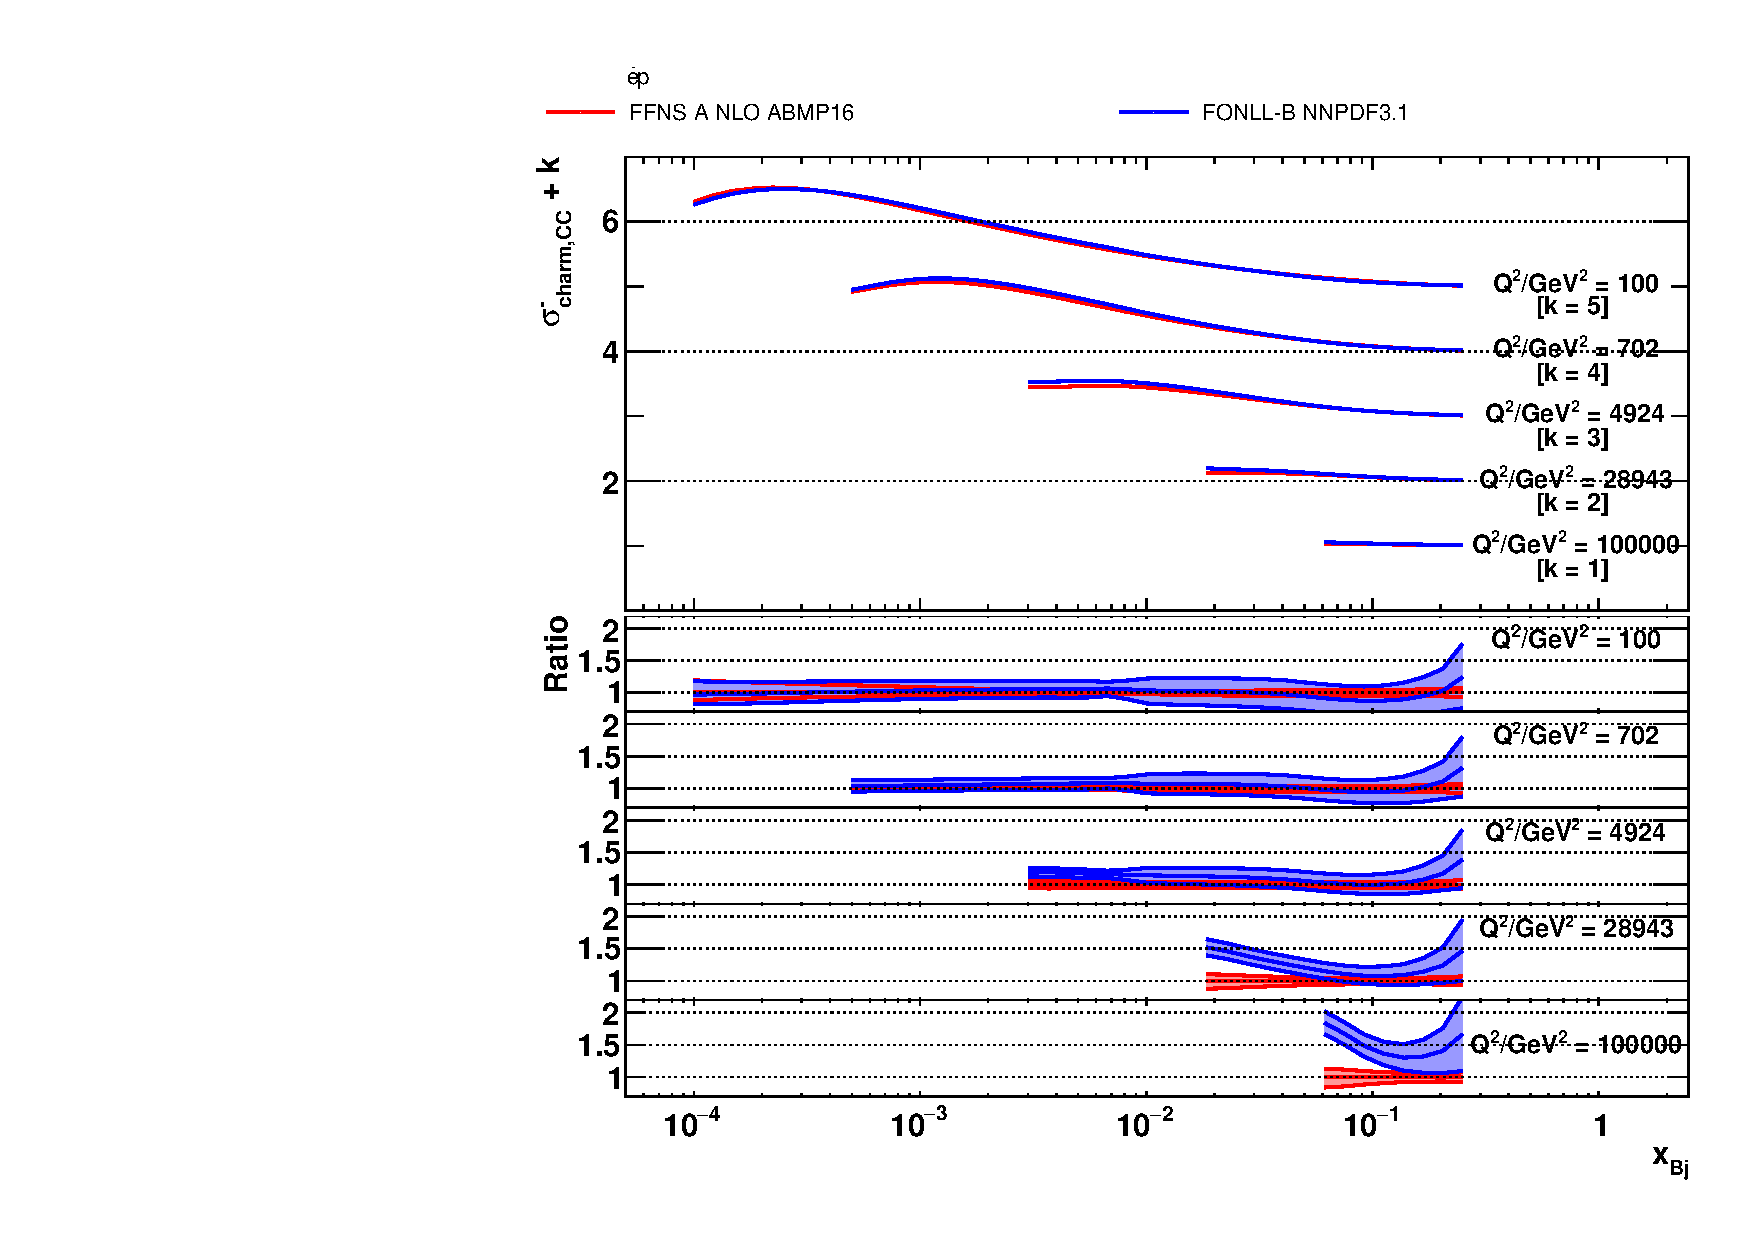
\includegraphics[width=0.50\textwidth]{pics/final/plot-sigmared-x-em.pdf}}}
    \caption{The theoretical predictions with their total
      uncertainties for charm CC production at the LHeC as a function
      of \xbj for different values of $Q^2$ calculated in the \ffns
      and \fonll schemes. The bottom panels display the theoretical
      predictions normalized to the nominal values of the \ffns
      predictions.}
    \label{fig:thpred-x}
\end{figure}

\begin{figure}
    \centering
    \centering{{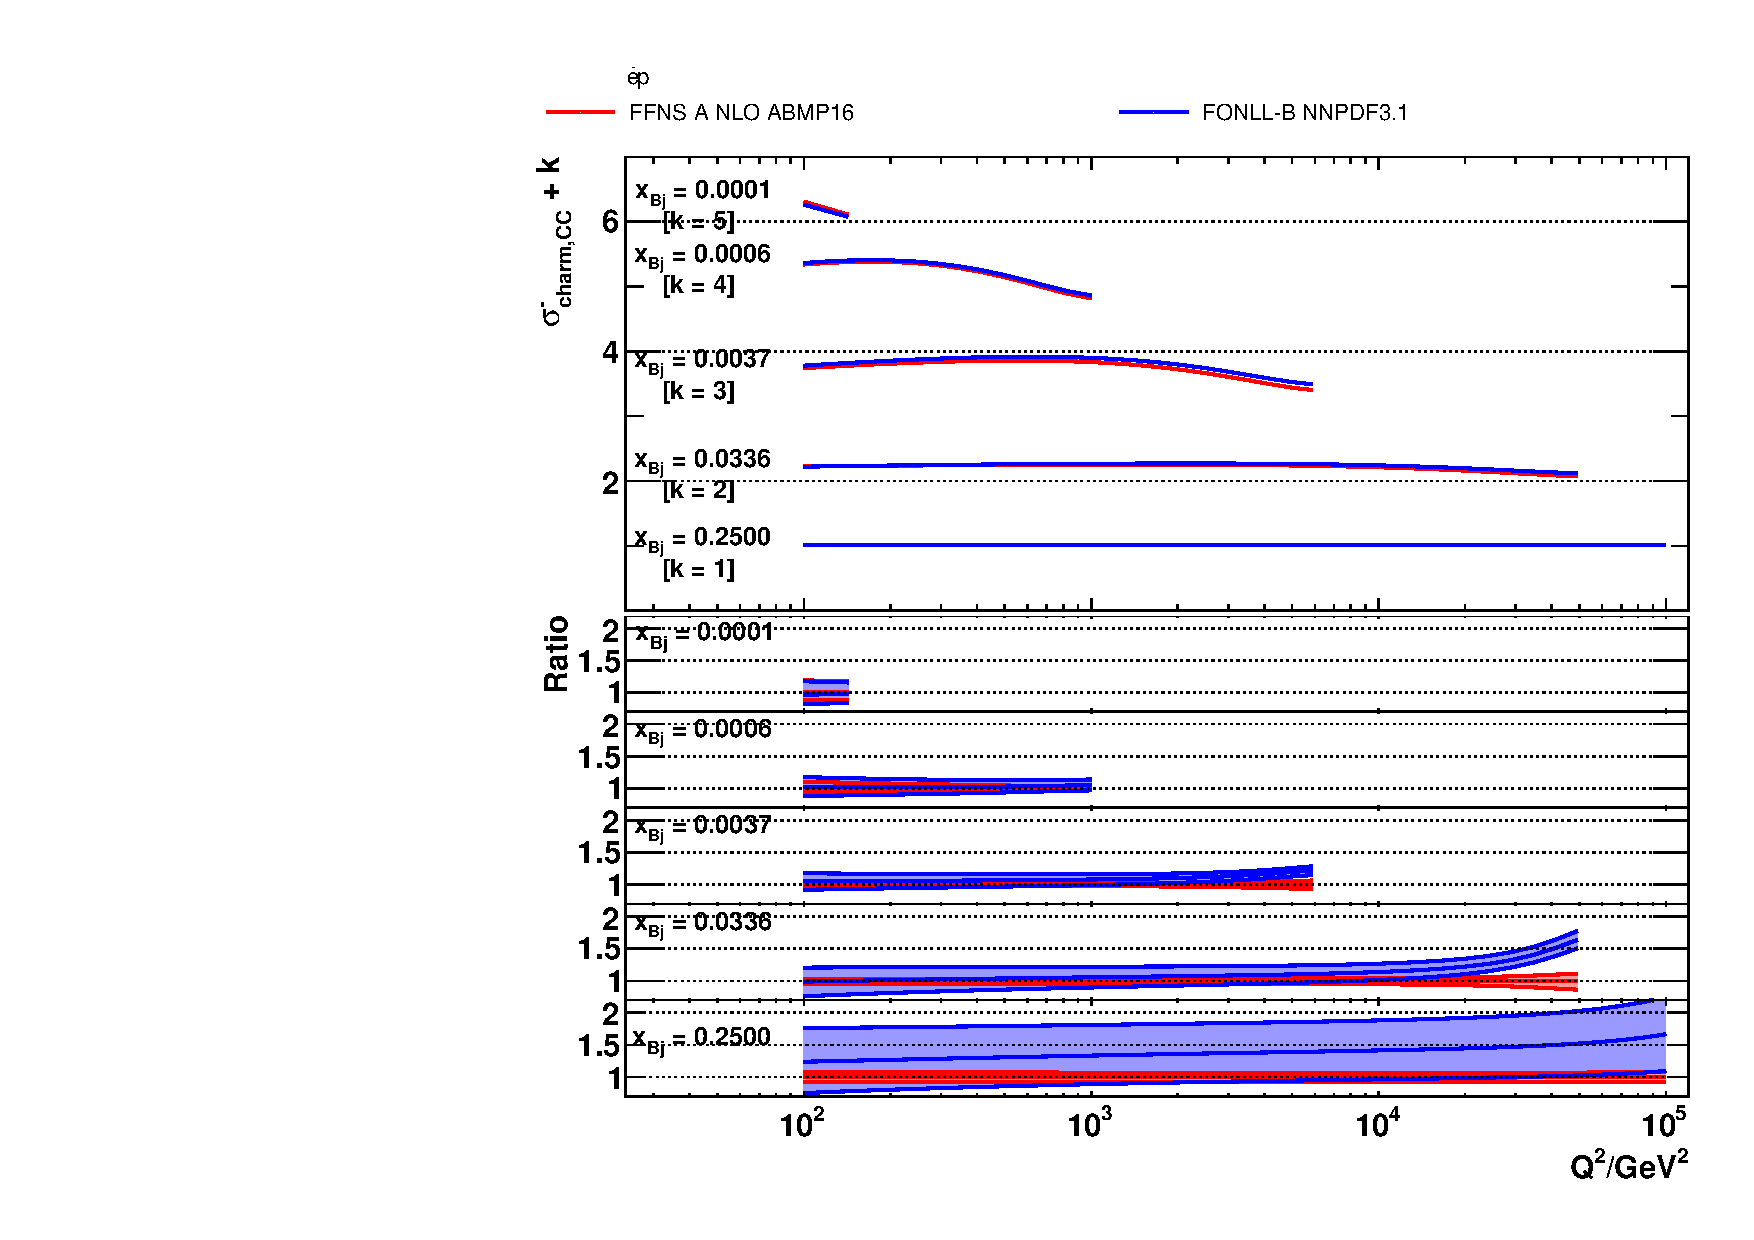
\includegraphics[width=0.50\textwidth]{pics/final/plot-sigmared-q2-em.pdf}}}
    \caption{The theoretical predictions with their total
      uncertainties for charm CC production at the LHeC as a function
      of $Q^2$ for different values of \xbj calculated in the \ffns
      and \fonll schemes. The bottom panels display the theoretical
      predictions normalized to the nominal values of the \ffns
      predictions.}
    \label{fig:thpred-q2}
\end{figure}

\begin{figure}
    \centering
    \centering{{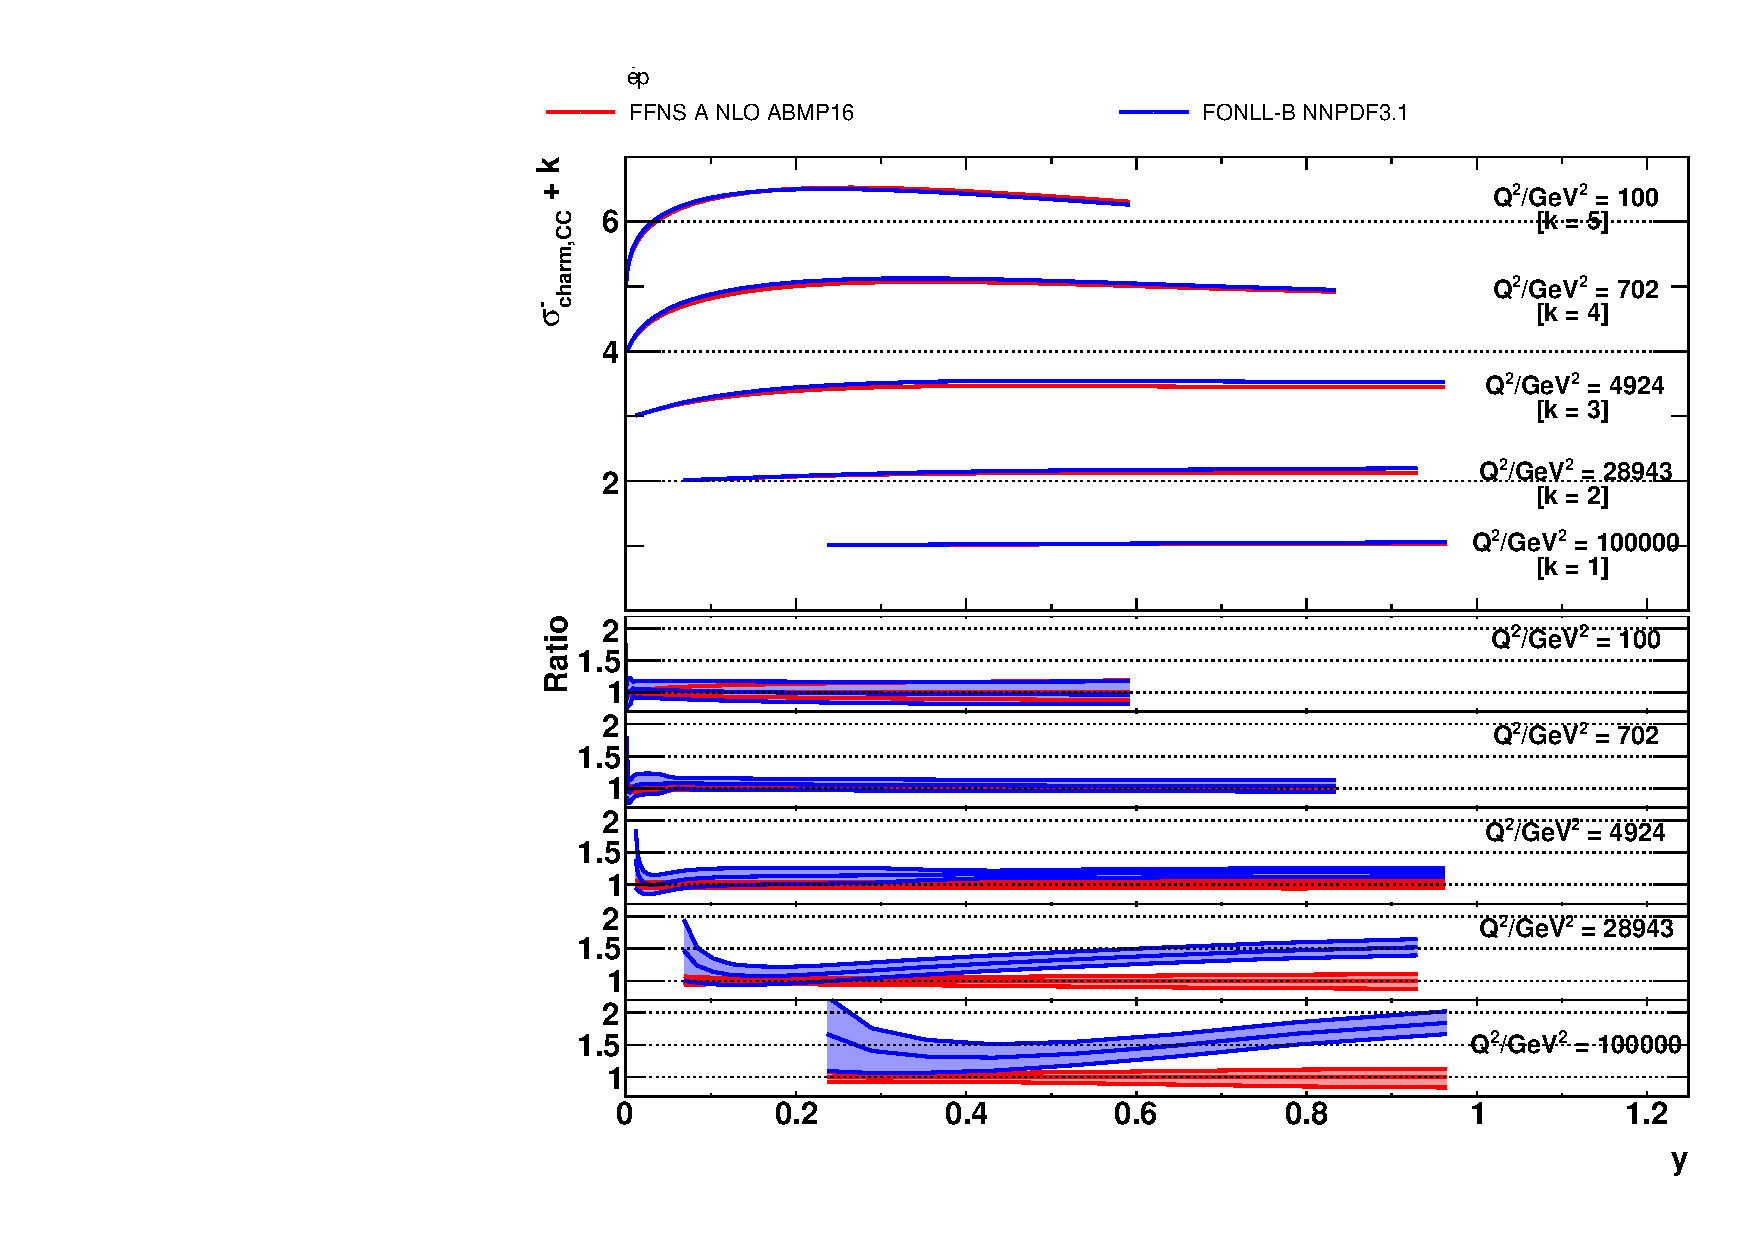
\includegraphics[width=0.50\textwidth]{pics/final/plot-sigmared-y-em.pdf}}}
    \caption{The theoretical predictions with their total
      uncertainties for charm CC production at the LHeC as a function
      of $y$ for different values of $Q^2$ calculated in the \ffns and
      \fonll schemes. The bottom panels display the theoretical
      predictions normalized to the nominal values of the \ffns
      predictions.}
    \label{fig:thpred-y}
\end{figure}

To examine these differences further, in Fig.~\ref{fig:thpred-q2-unc}
we separately compute PDF and scale uncertainties (setting
$\mu_\mathrm{r}=\mu_\mathrm{f}=\mu$) of the charm CC cross section as
a function of $Q^2$ for different values of \xbj calculated in the
\ffns and \fonll scheme.
%
%% Additionally, Fig.~\ref{fig:thpred-q2-varmu} shows the impact of
%% separate scale variations $\mu_\mathrm{r}$ and $\mu_\mathrm{f}$ in the
%% two schemes.

Comparing the two schemes, the larger variation of the \fonll scheme
reflects the larger PDF uncertainty of the underlying PDF sets used:
ABMP16 for \ffns and NNPDF3.1 for \fonll.
%
This difference is most evident in Fig.~\ref{fig:thpred-q2-unc} which
specifically separates out the PDF uncertainty, and reflects the
independent inputs and assumptions used in the different PDF
extractions.

Examining the results of Fig.~\ref{fig:thpred-q2-unc}, we also observe
some other interesting features.
%
For both of the calculations, the PDF uncertainties are relatively stable
across the  $Q^2$ range for fixed \xbj, but tend to increase at larger \xbj values.
%
As is well known, in pQCD calculations the effect of scale variations
is indicative of the convergence of the series.
%
We observe that the scale uncertainties for the \fonll scheme
uniformly decrease with increasing $Q^2$.
%
For the \ffns scheme, the scale uncertainties decrease for small \xbj
values but increase with $Q^2$ at intermediate values of \xbj.
%
Additional details are shown in Fig.~\ref{fig:thpred-q2-varmu} where
we separately vary $\mu_\mathrm{r}$ and $\mu_\mathrm{f}$ for the
\fonll scheme. Here we note that the uncertainty associated to
$\mu_\mathrm{r}$ is very small and the total scale uncertainty is
dominated by the variations of $\mu_\mathrm{f}$ which is tied to the
PDFs, $f_i(x,\mu_\mathrm{f})$.
%
For the \ffns in \xfitter, it is not possible to separately vary
$\mu_\mathrm{r}$ and $\mu_\mathrm{f}$ in the current implementation,
so the separate uncertainties can only be inferred by comparison to
the \fonll case.

\begin{figure*}
    \centering
    \centering{{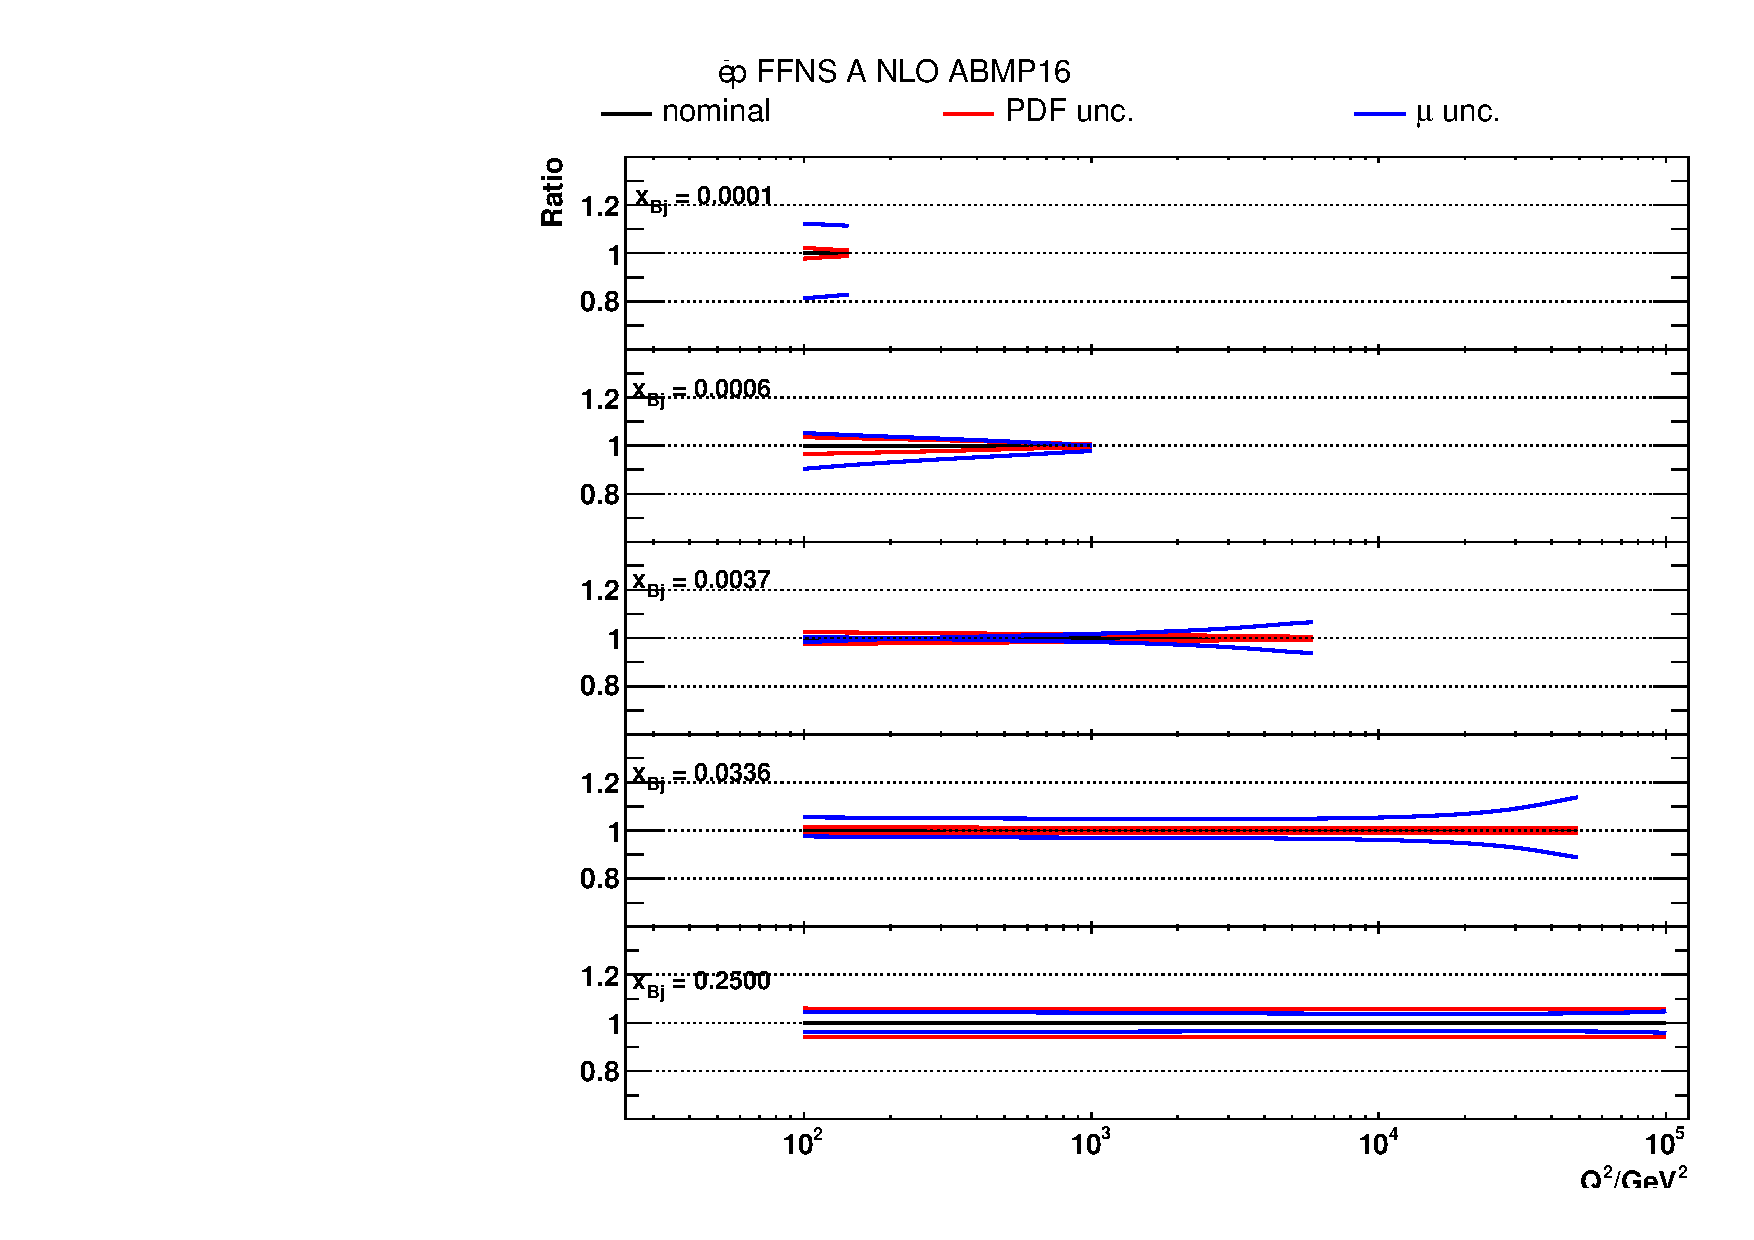
\includegraphics[width=0.49\textwidth]{pics/final/plot-unc-q2-em-FFABM.pdf}}}
    \centering{{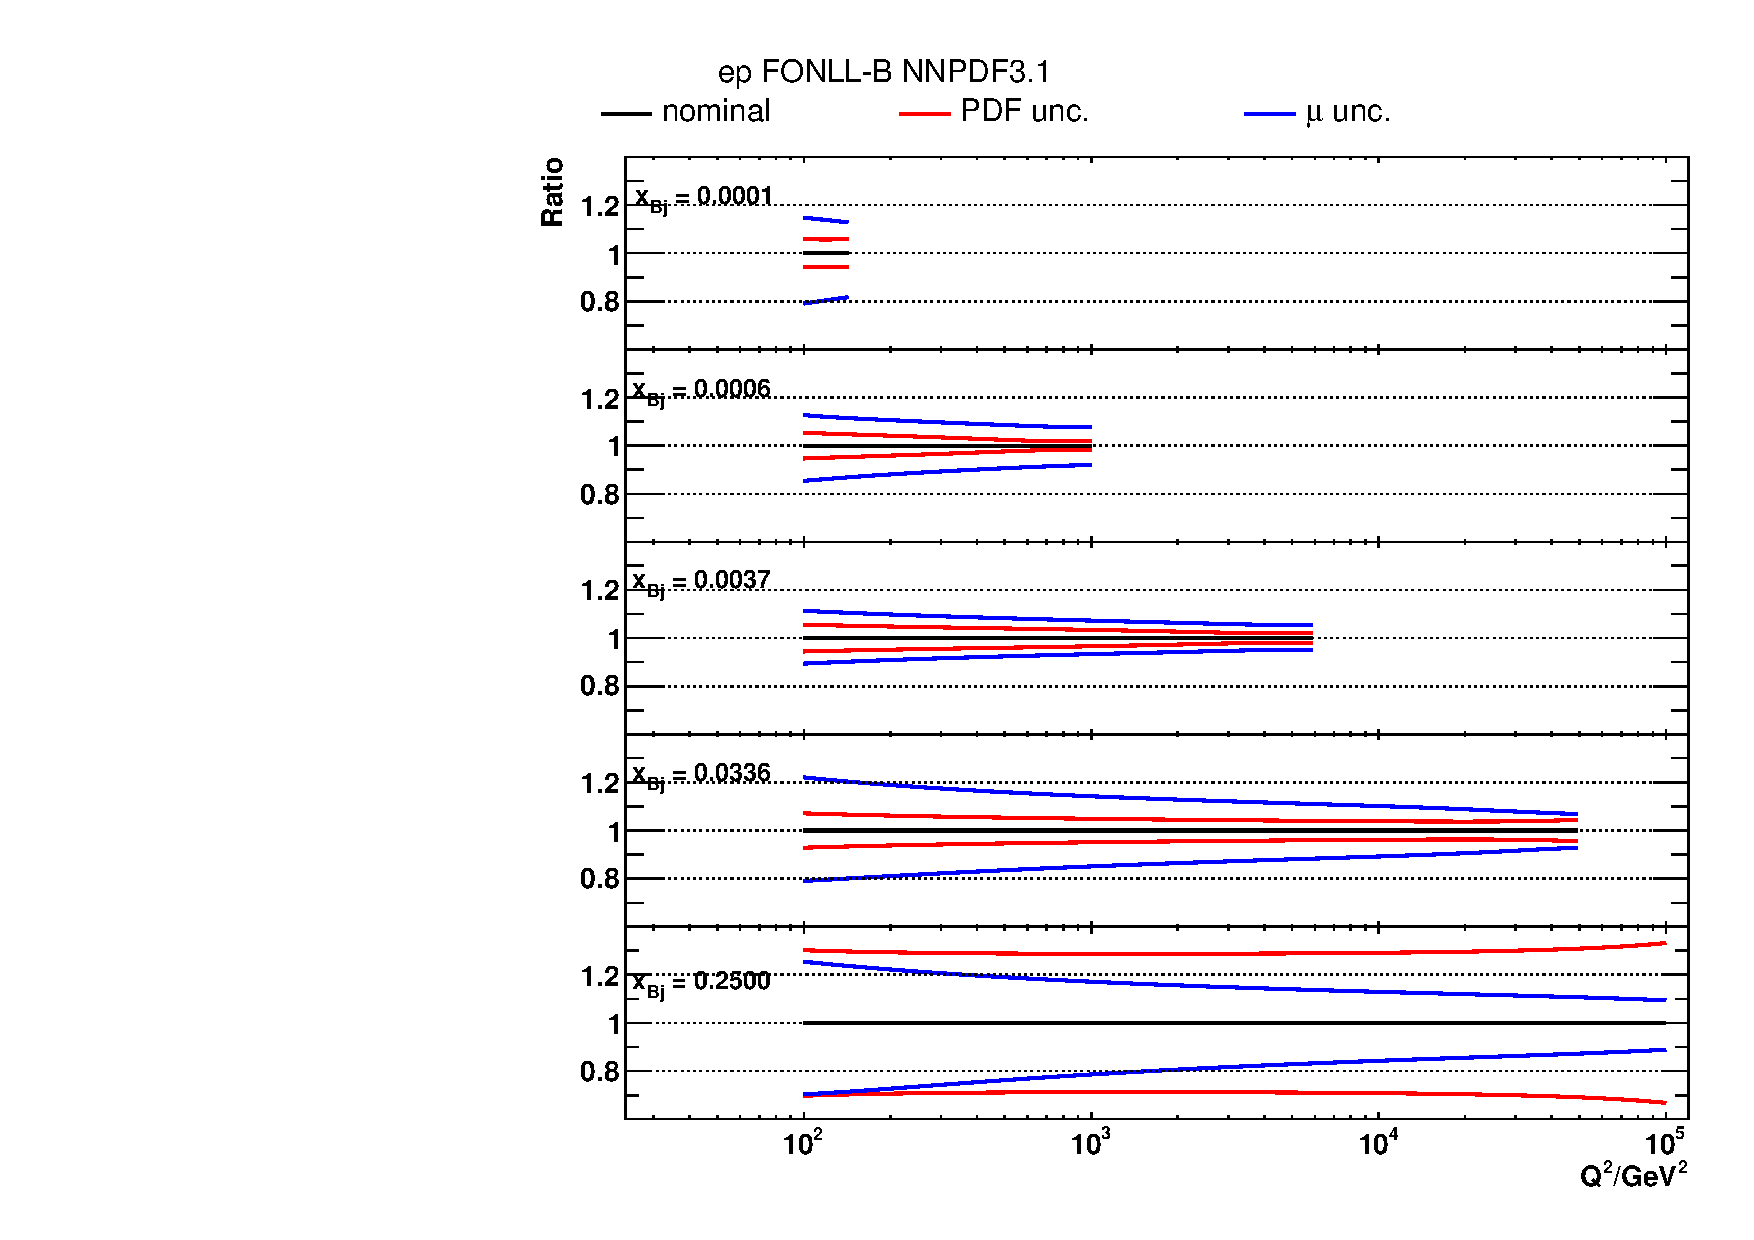
\includegraphics[width=0.49\textwidth]{pics/final/plot-unc-q2-em-FONLL.pdf}}}
    \caption{Relative theoretical uncertainties of charm CC
      predictions for the LHeC as a function of $Q^2$ for different
      values of \xbj calculated in the \ffns and \fonll schemes. The
      PDF and scale uncertainties are shown separately.}
    \label{fig:thpred-q2-unc}
\end{figure*}

\begin{figure*}
    \centering
    \centering{{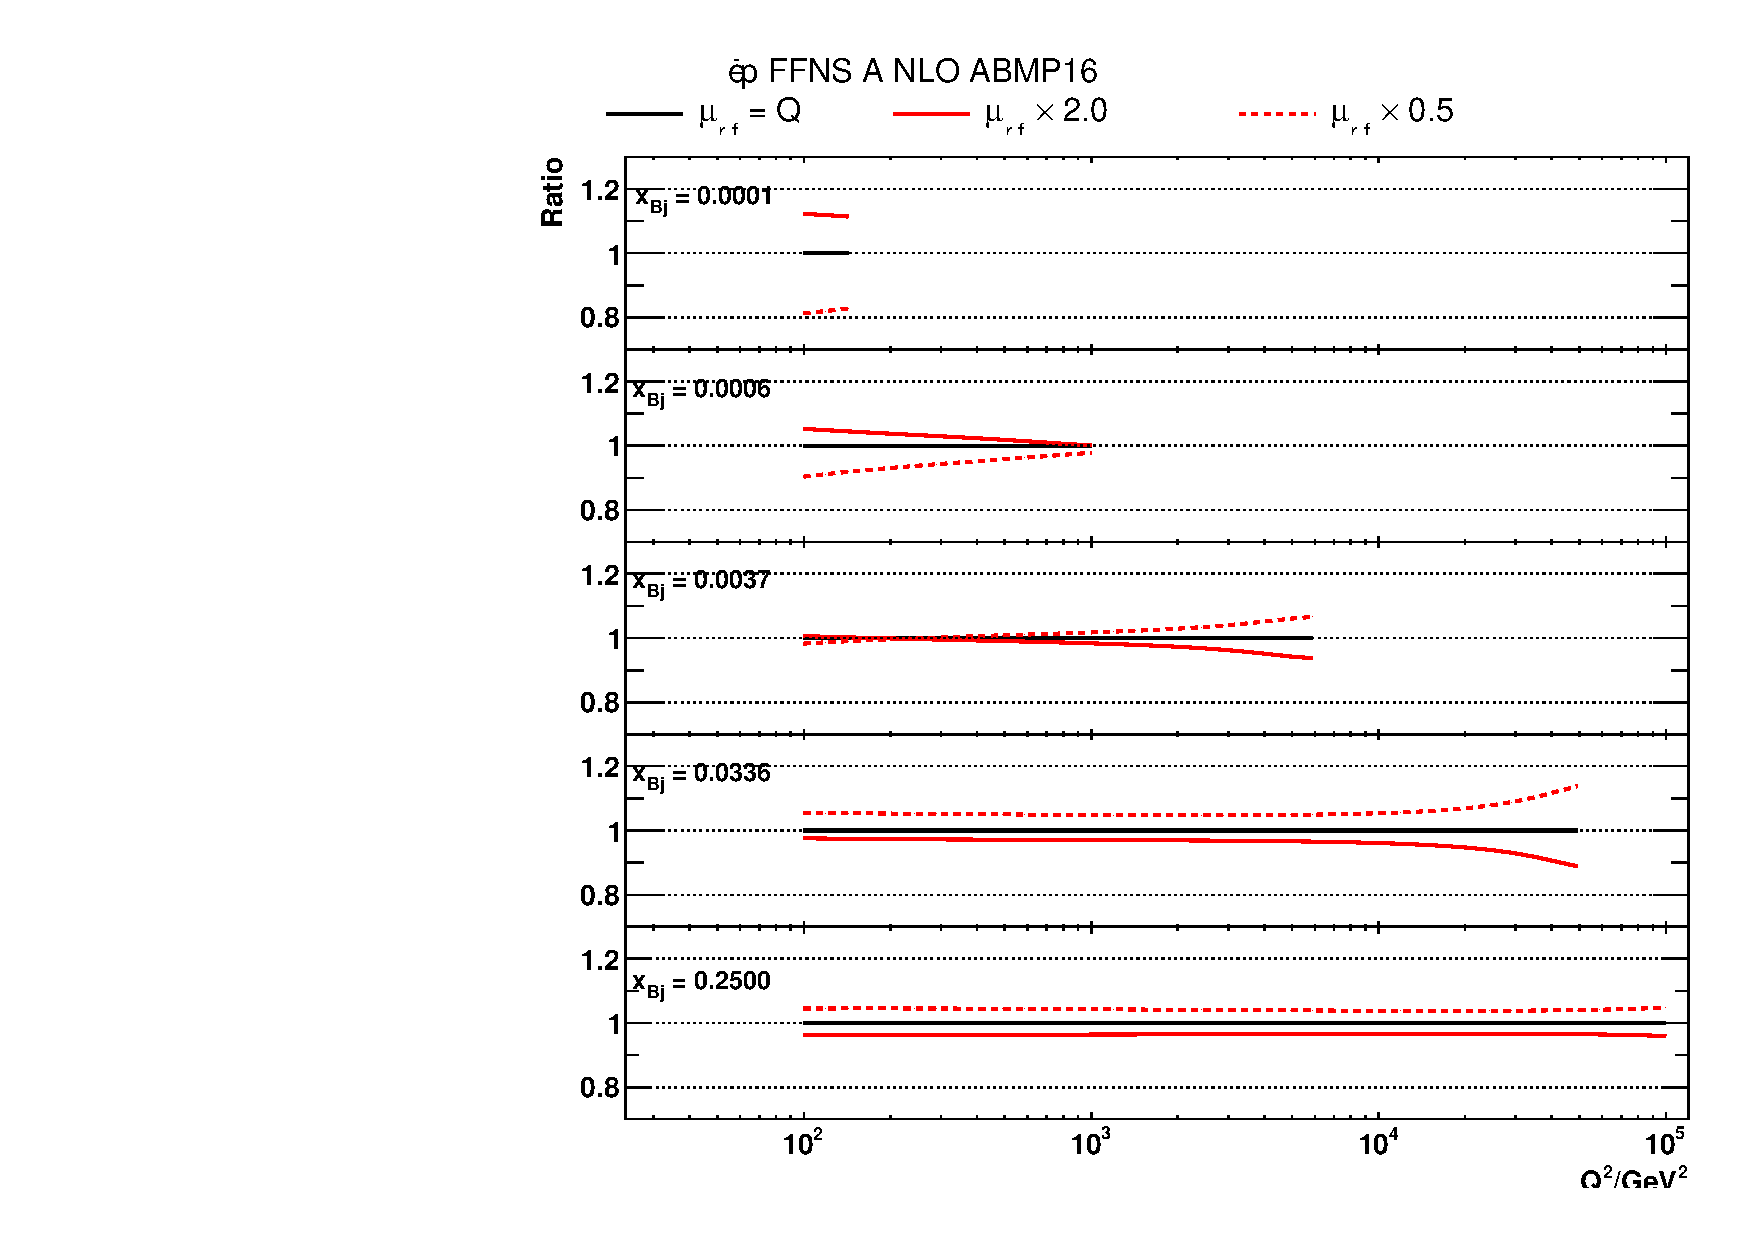
\includegraphics[width=0.49\textwidth]{pics/final/plot-varmu-q2-em-FFABM.pdf}}}
    \centering{{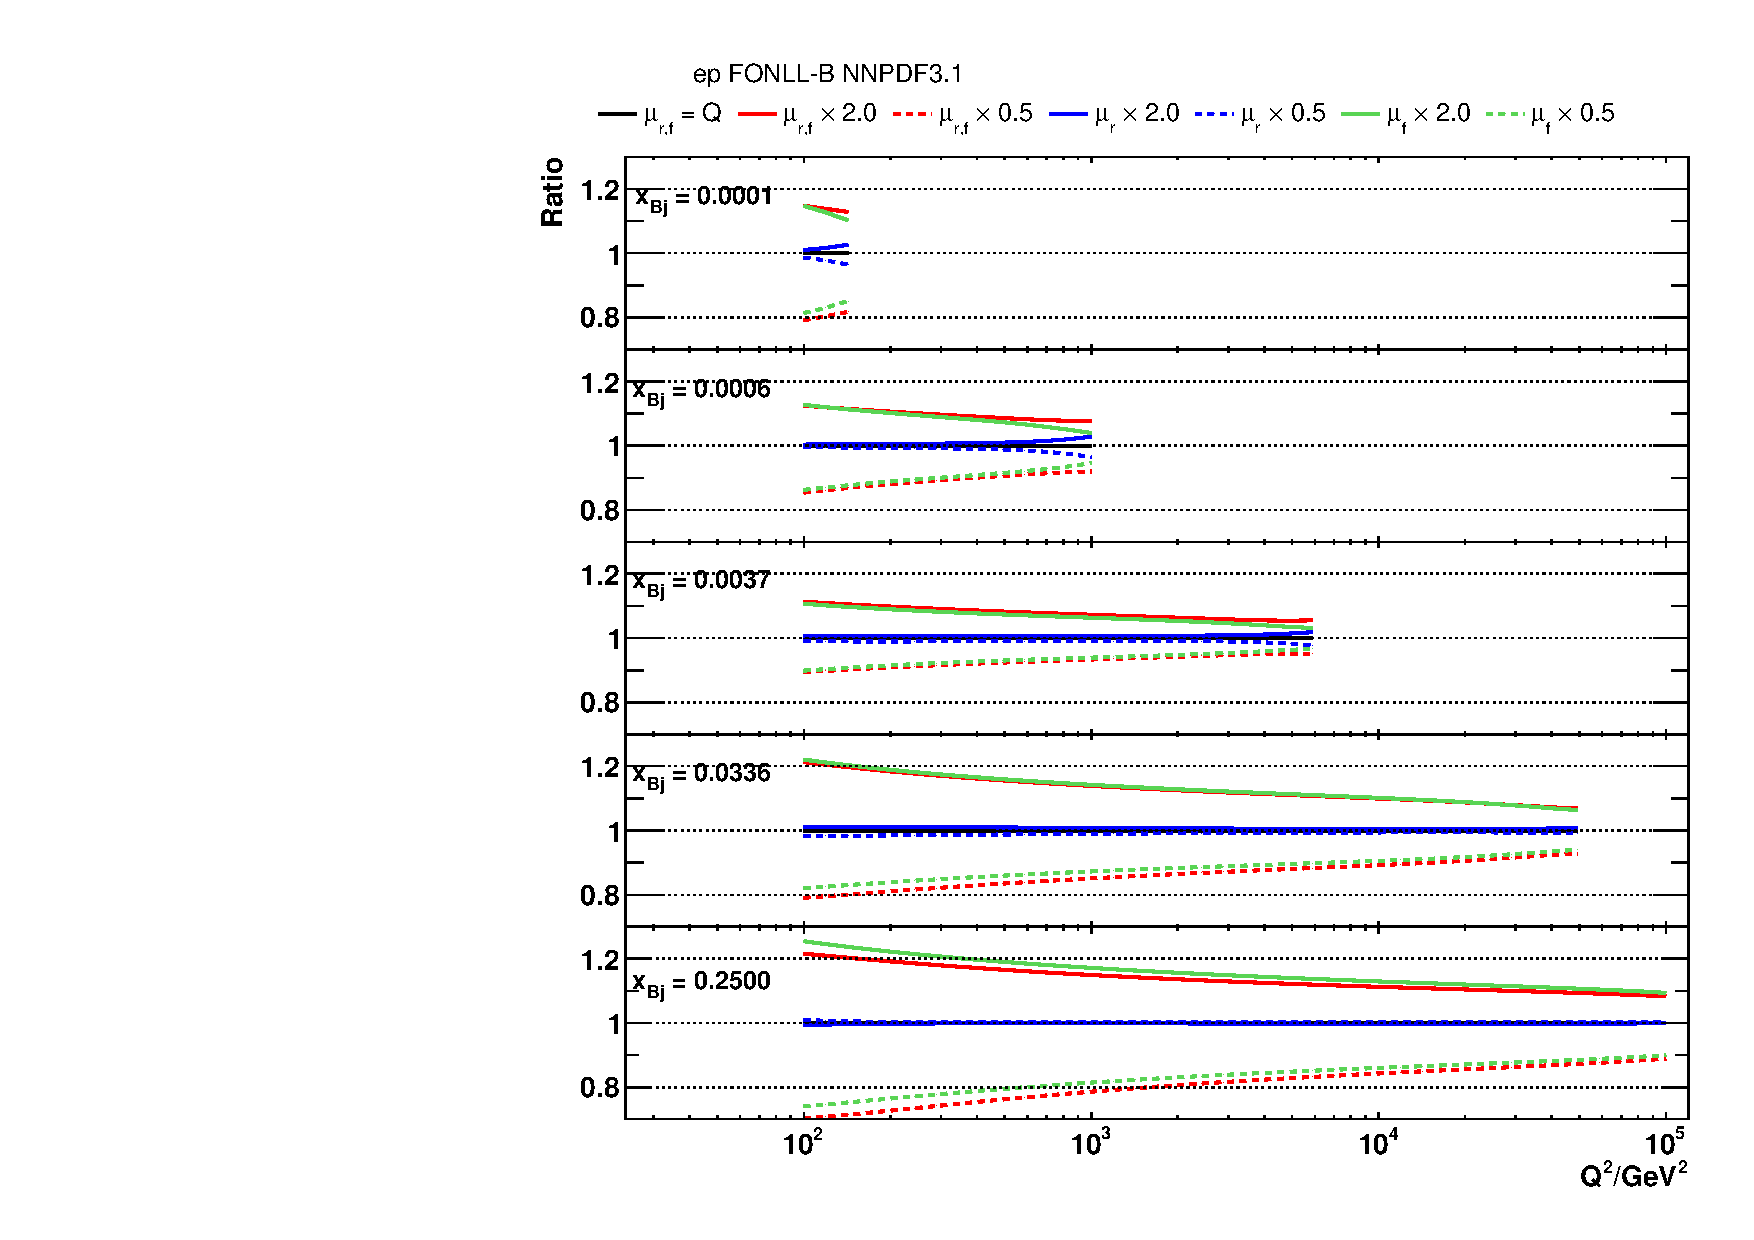
\includegraphics[width=0.49\textwidth]{pics/final/plot-varmu-q2-em-FONLL.pdf}}}
    \caption{The impact of separate scale variations on charm CC
      predictions for the LHeC as a function of $Q^2$ for different
      values of \xbj calculated in the \ffns and \fonll schemes.}
    \label{fig:thpred-q2-varmu}
\end{figure*}

%%%%%%%%%%%%%%%%%%%%%%%%



%%%%%%%%%%%%%%%%%%%%%%%%%%%%%%%%%%%%%%%%%

\begin{figure*}
  \centering
  \centering{{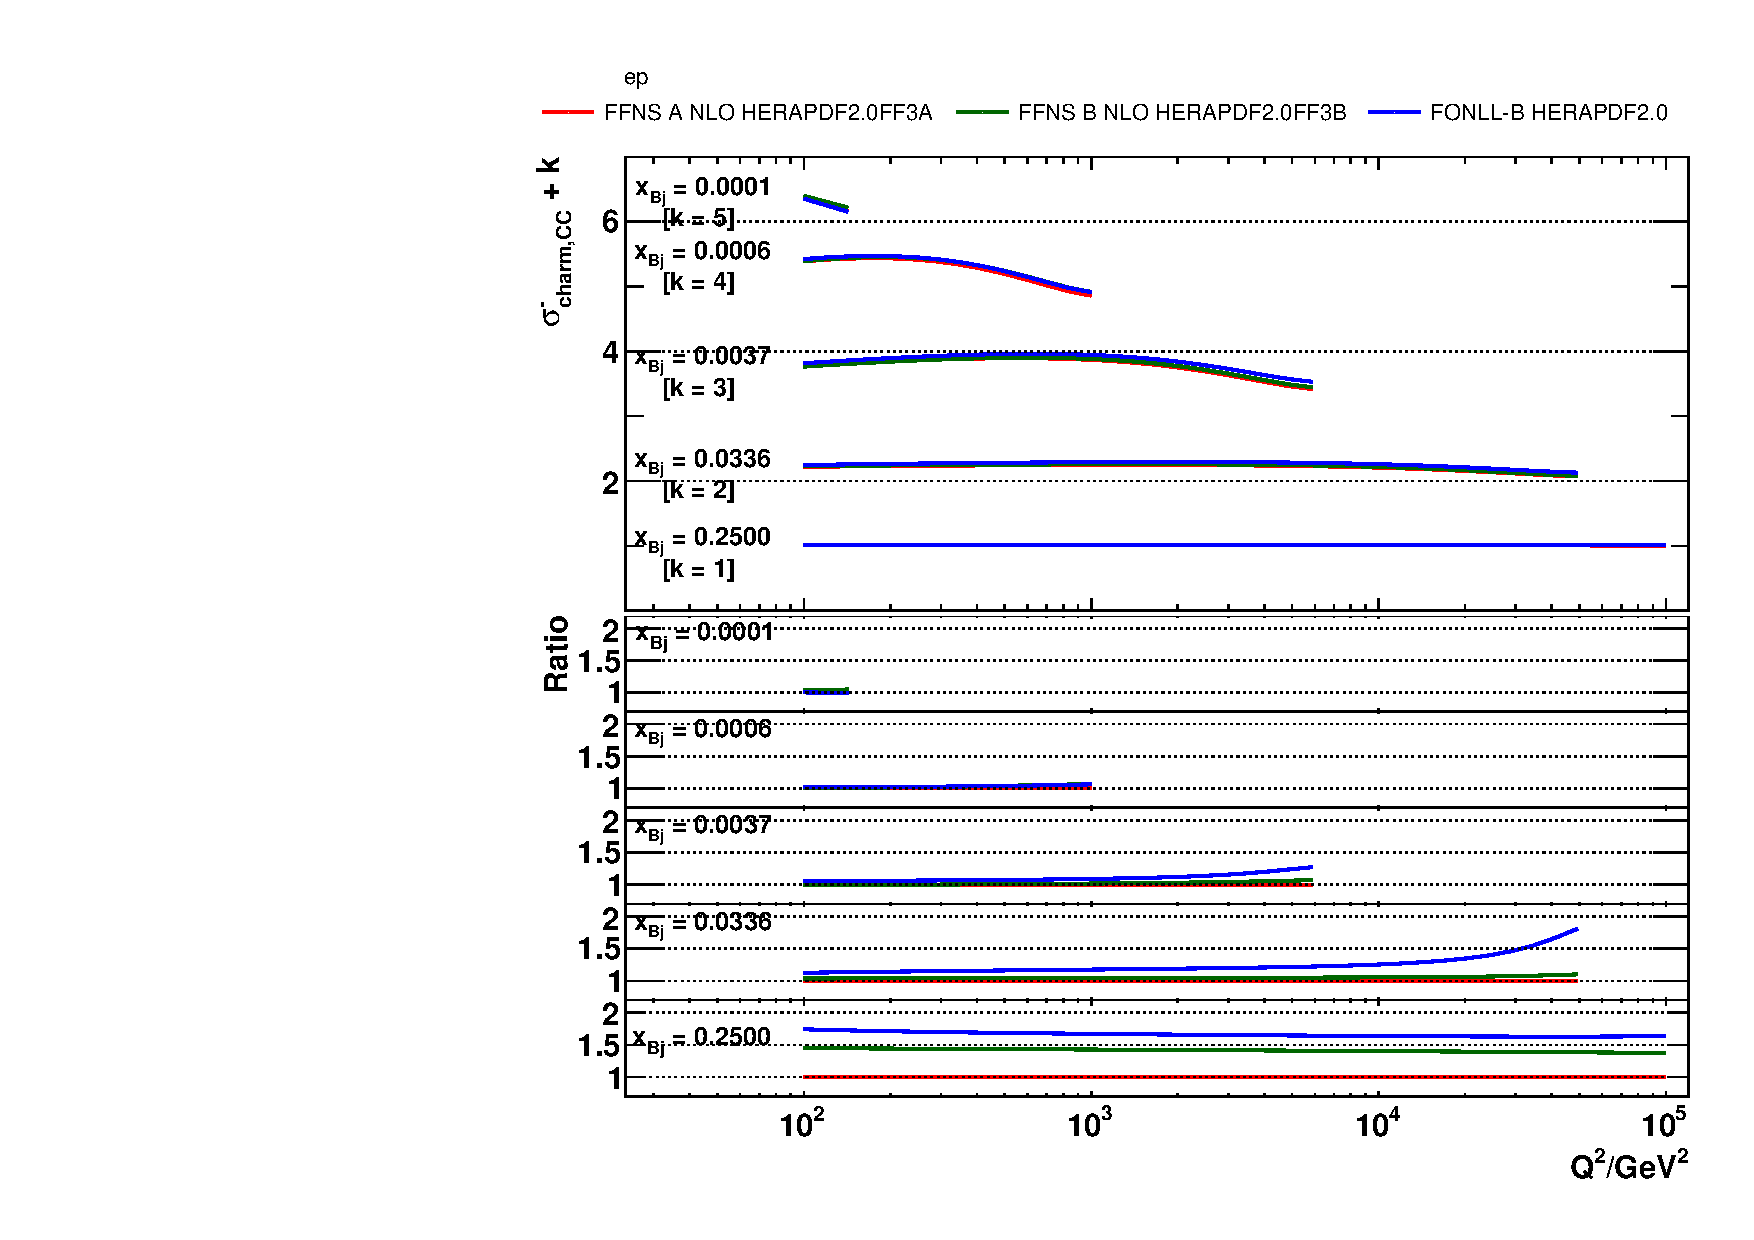
\includegraphics[width=0.49\textwidth]{pics/final/plot-FF3ABFONLL-q2-em.pdf}}}
  \centering{{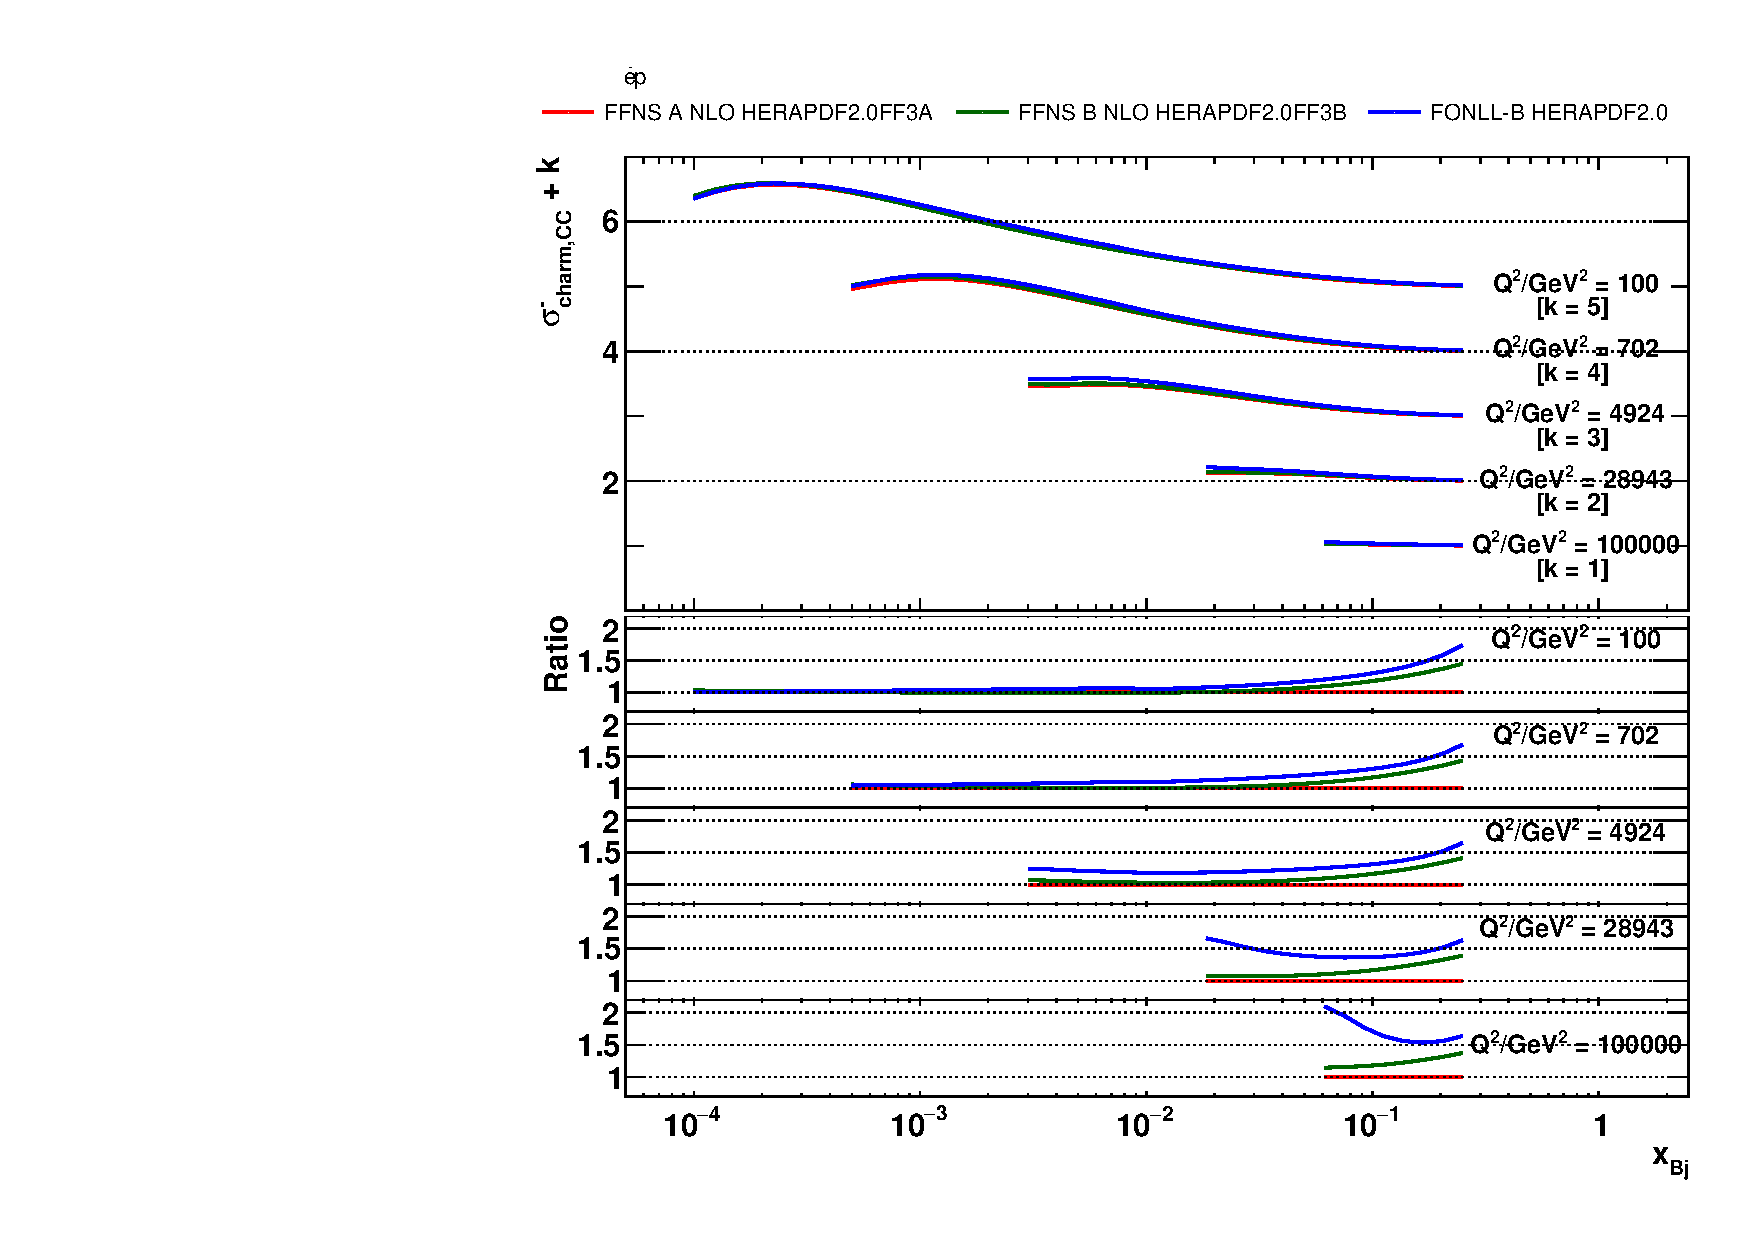
\includegraphics[width=0.49\textwidth]{pics/final/plot-FF3ABFONLL-x-em.pdf}}}
  \centering{{\includegraphics[width=0.49\textwidth]{pics/final/plot-FF3ABFONLL-y-em.pdf}}}
  \caption{The theoretical predictions for CC charm production at the
    LHeC as a function of $Q^2$ ($\xbj$, $y$) for different values of
    $\xbj$ ($\xbj$, $Q^2$) obtained using the HERAPDF2.0 PDF sets in
    the \ffns, \ffnsb and \fonll schemes. The bottom panels display the
    theoretical predictions normalized to the nominal values of the
    \ffns predictions.}
  \label{fig:thpred-ff3abfonll}
\end{figure*}

%%%%%%%%%%%%%%%%%%%%%%%%%%%%%%%%%%%%%%%%%



%%%%%%%%%%%%%%%%%%%%%%%%%%%%%%%%%%%%%%%%%
\subsection{Additional comparisons}
\label{sec:compareII}

To further explore whether the differences between the two sets of
theoretical predictions are due to the different treatment of heavy
quarks or to the different PDF sets, theoretical calculations in \ffns
and \fonll are repeated with the HERAPDF2.0 PDF sets extracted from
the HERA DIS data~\cite{Abramowicz:2015mha}.
%
Predictions in the \ffnsb scheme are also produced using the \ffthreeb
PDF set and the \ffnsb matrix elements, which are equivalent to the
\ffns matrix elements at NLO for CC charm production. The results are
displayed in Fig.~\ref{fig:thpred-ff3abfonll}. The differences between
\ffns and \fonll are similar to those displayed in
Figs.~\ref{fig:thpred-x}-\ref{fig:thpred-y} and demonstrate that these
differences arise from the different treatment of the heavy quarks in
the two schemes. The \ffnsb predictions lie between the \ffns and
\fonll predictions, indicating that a large part of the difference
is due to the different treatment of heavy quarks in the running of
$\alpha_s$ at high \xbj or low $y$.


Furthermore, to investigate the impact of the NNLO corrections
available at $Q \gg m_c$ for the FFNS calculation, approximate NNLO
predictions are obtained using the \abmp NNLO PDF
set~\cite{Alekhin:2017kpj}. The results for the cross section as a
function of $Q^2$ for different values of \xbj are shown in
Fig.~\ref{fig:thpred-q2-nnlo}, where they are compared to the NLO
\ffns predictions from Fig.~\ref{fig:thpred-q2}. The NNLO corrections
do not exceed $10\%$ and thus cannot account for the differences
between the \ffns and \fonll theoretical predictions. Similar results
are observed for the cross sections as functions of other kinematic
variables.


%\begin{figure*}
%    \centering
%    \centering{{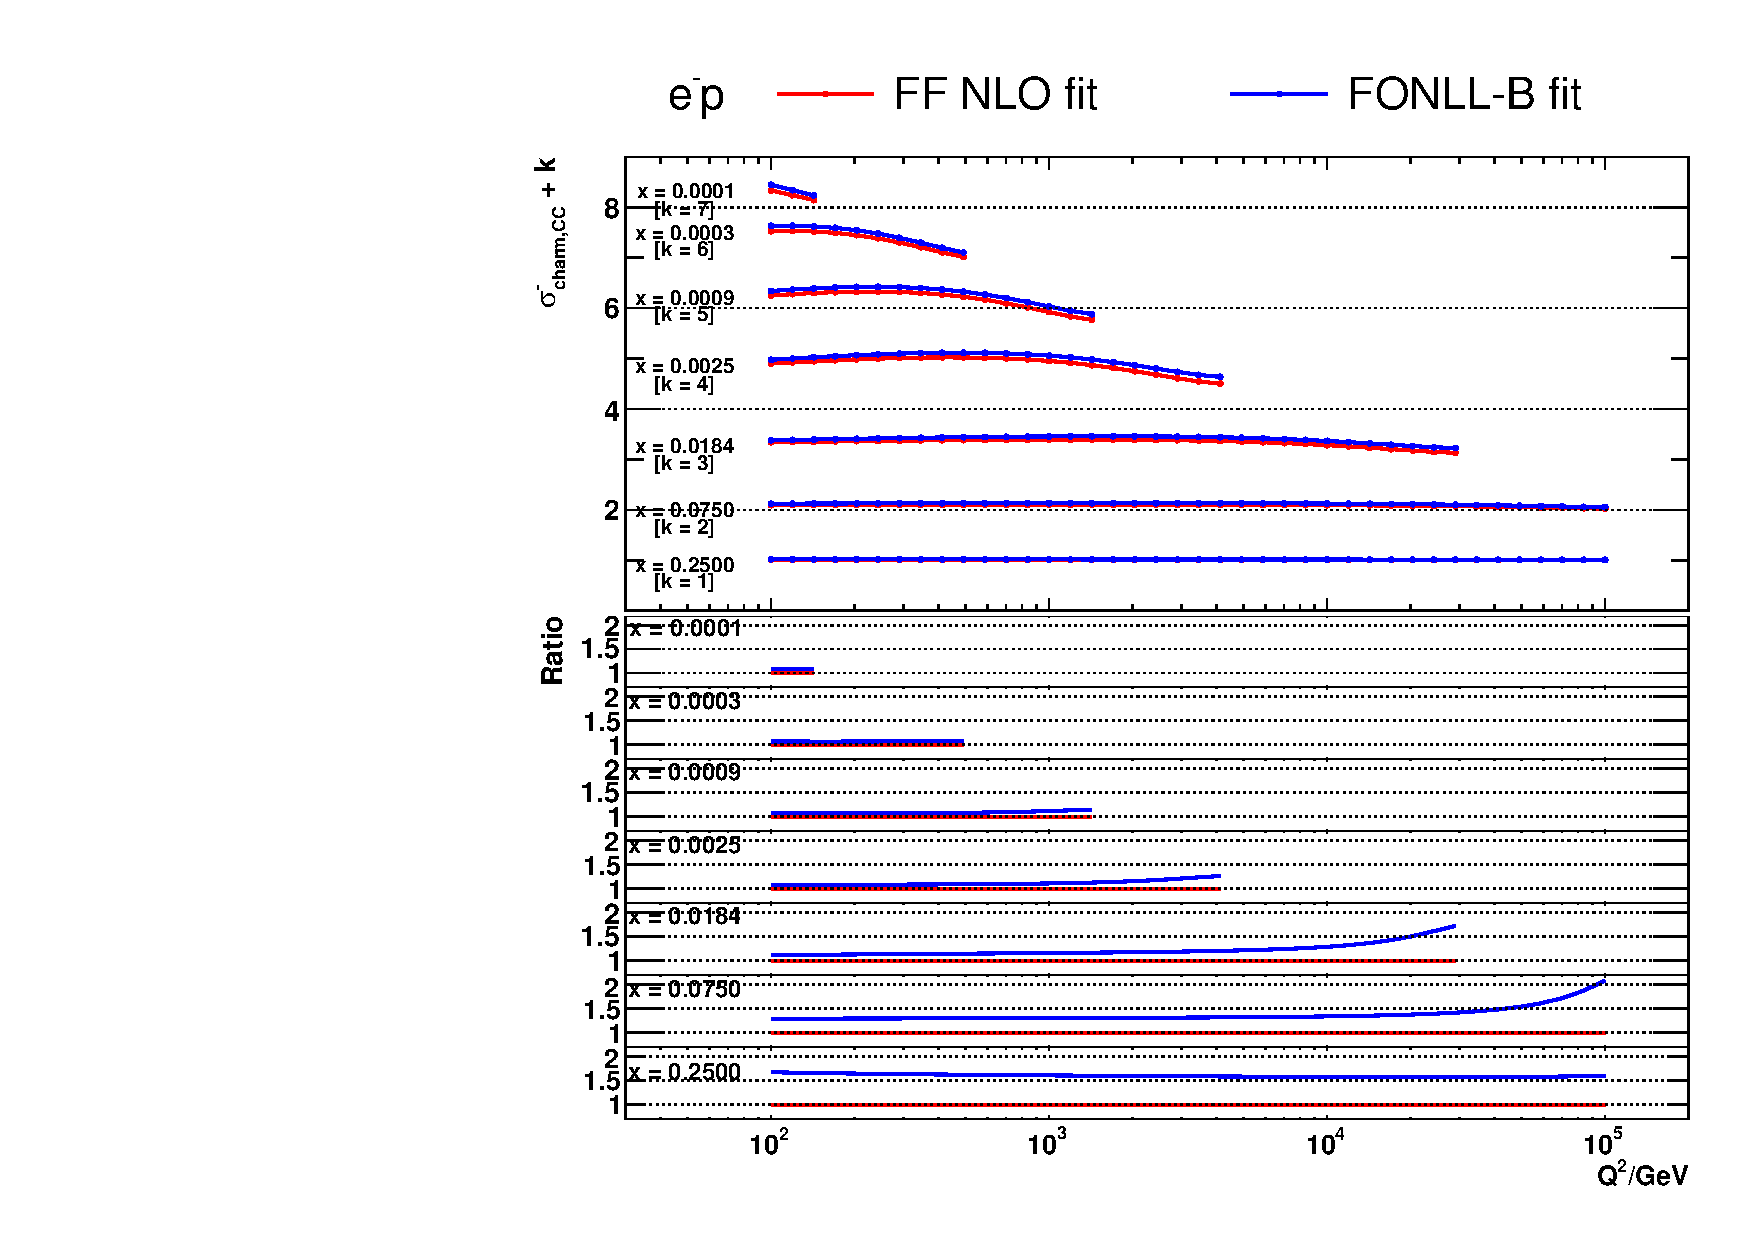
\includegraphics[width=0.49\textwidth]{pics/plots-191018/plot-fit-q2-em.pdf}}}
%    \centering{{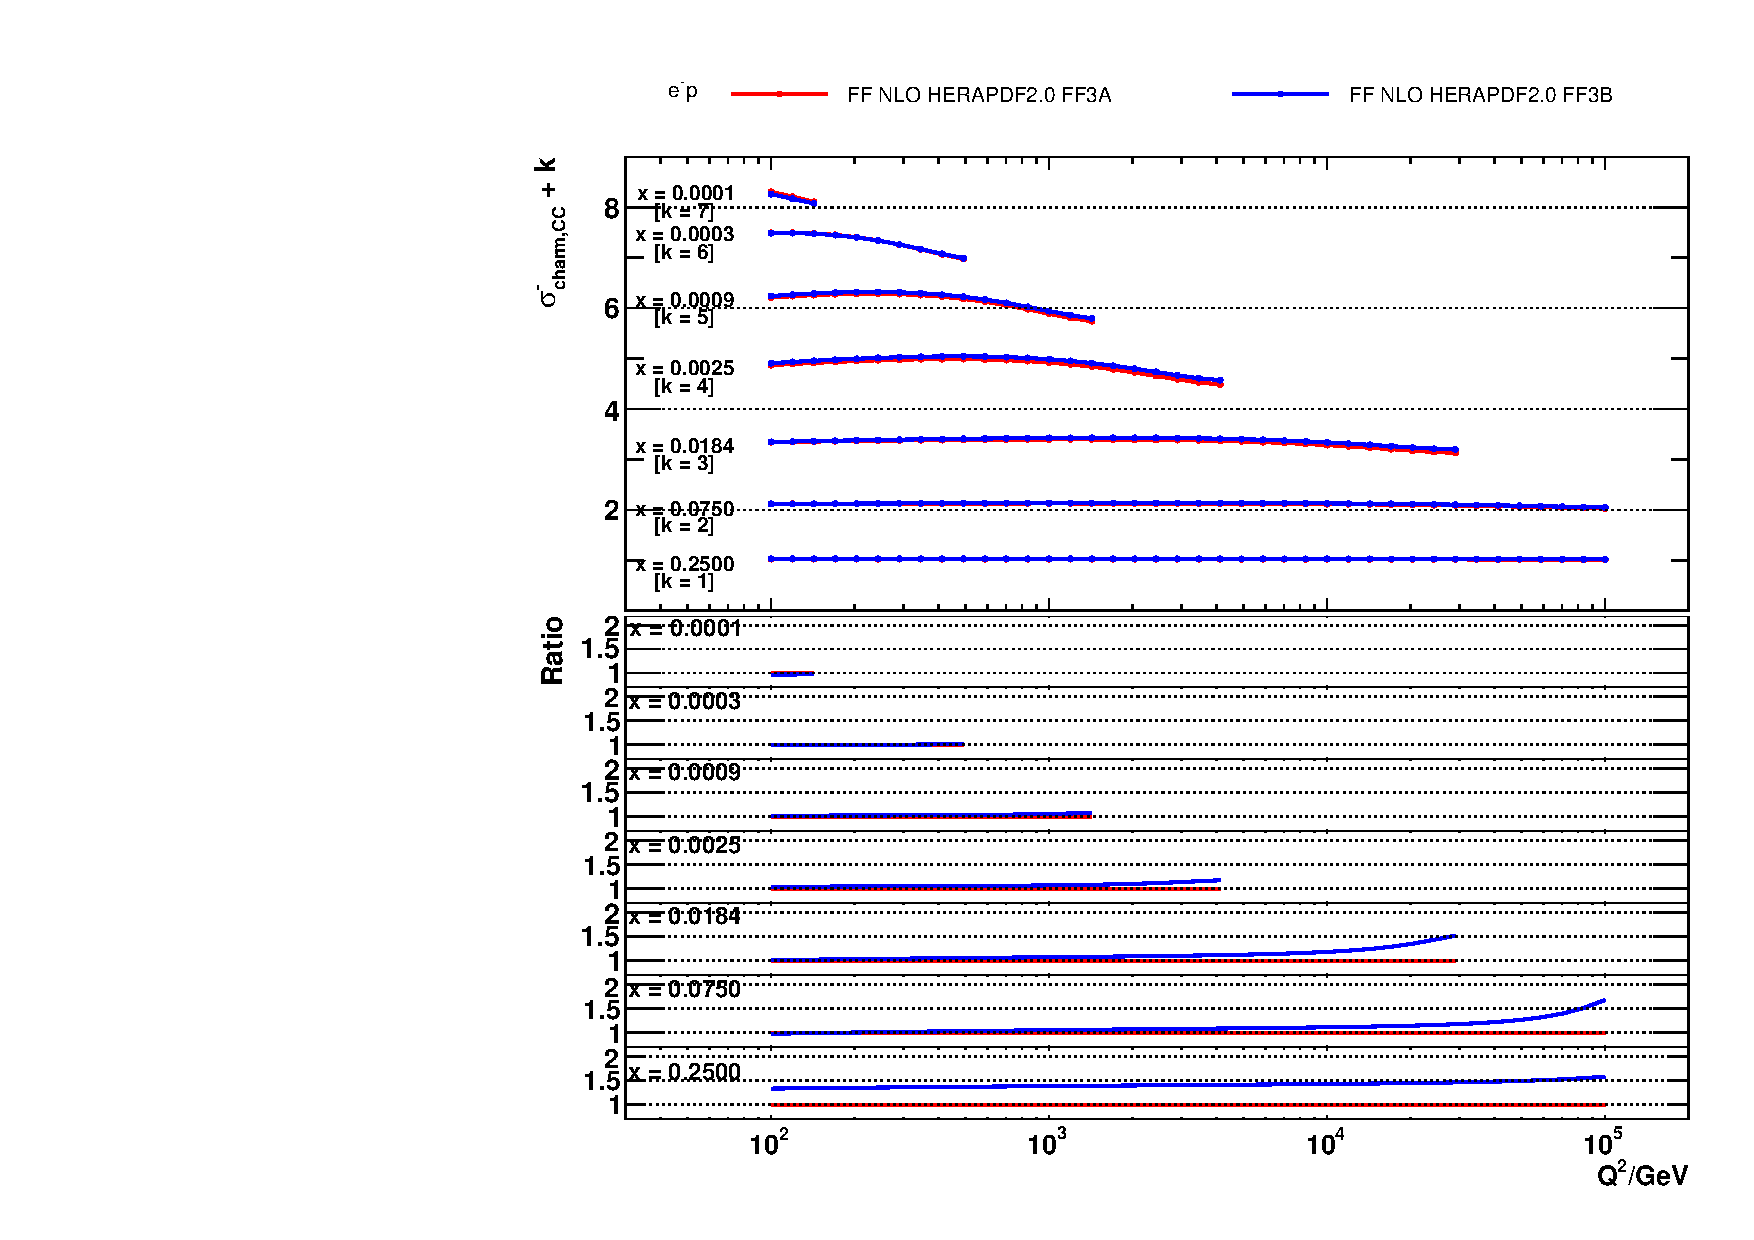
\includegraphics[width=0.49\textwidth]{pics/plots-191018/plot-FF3AB-q2-em.pdf}}}
%    \caption{(left) The theoretical predictions for charm CC production at the LHeC as a function of $Q^2$ for different values of $\xbj$. See Fig.~\ref{fig:thpred-fit-y} for further details.}
%    \label{fig:thpred-fit-q2}
%\end{figure*}
%
%\begin{figure*}
%    \centering
%    \centering{{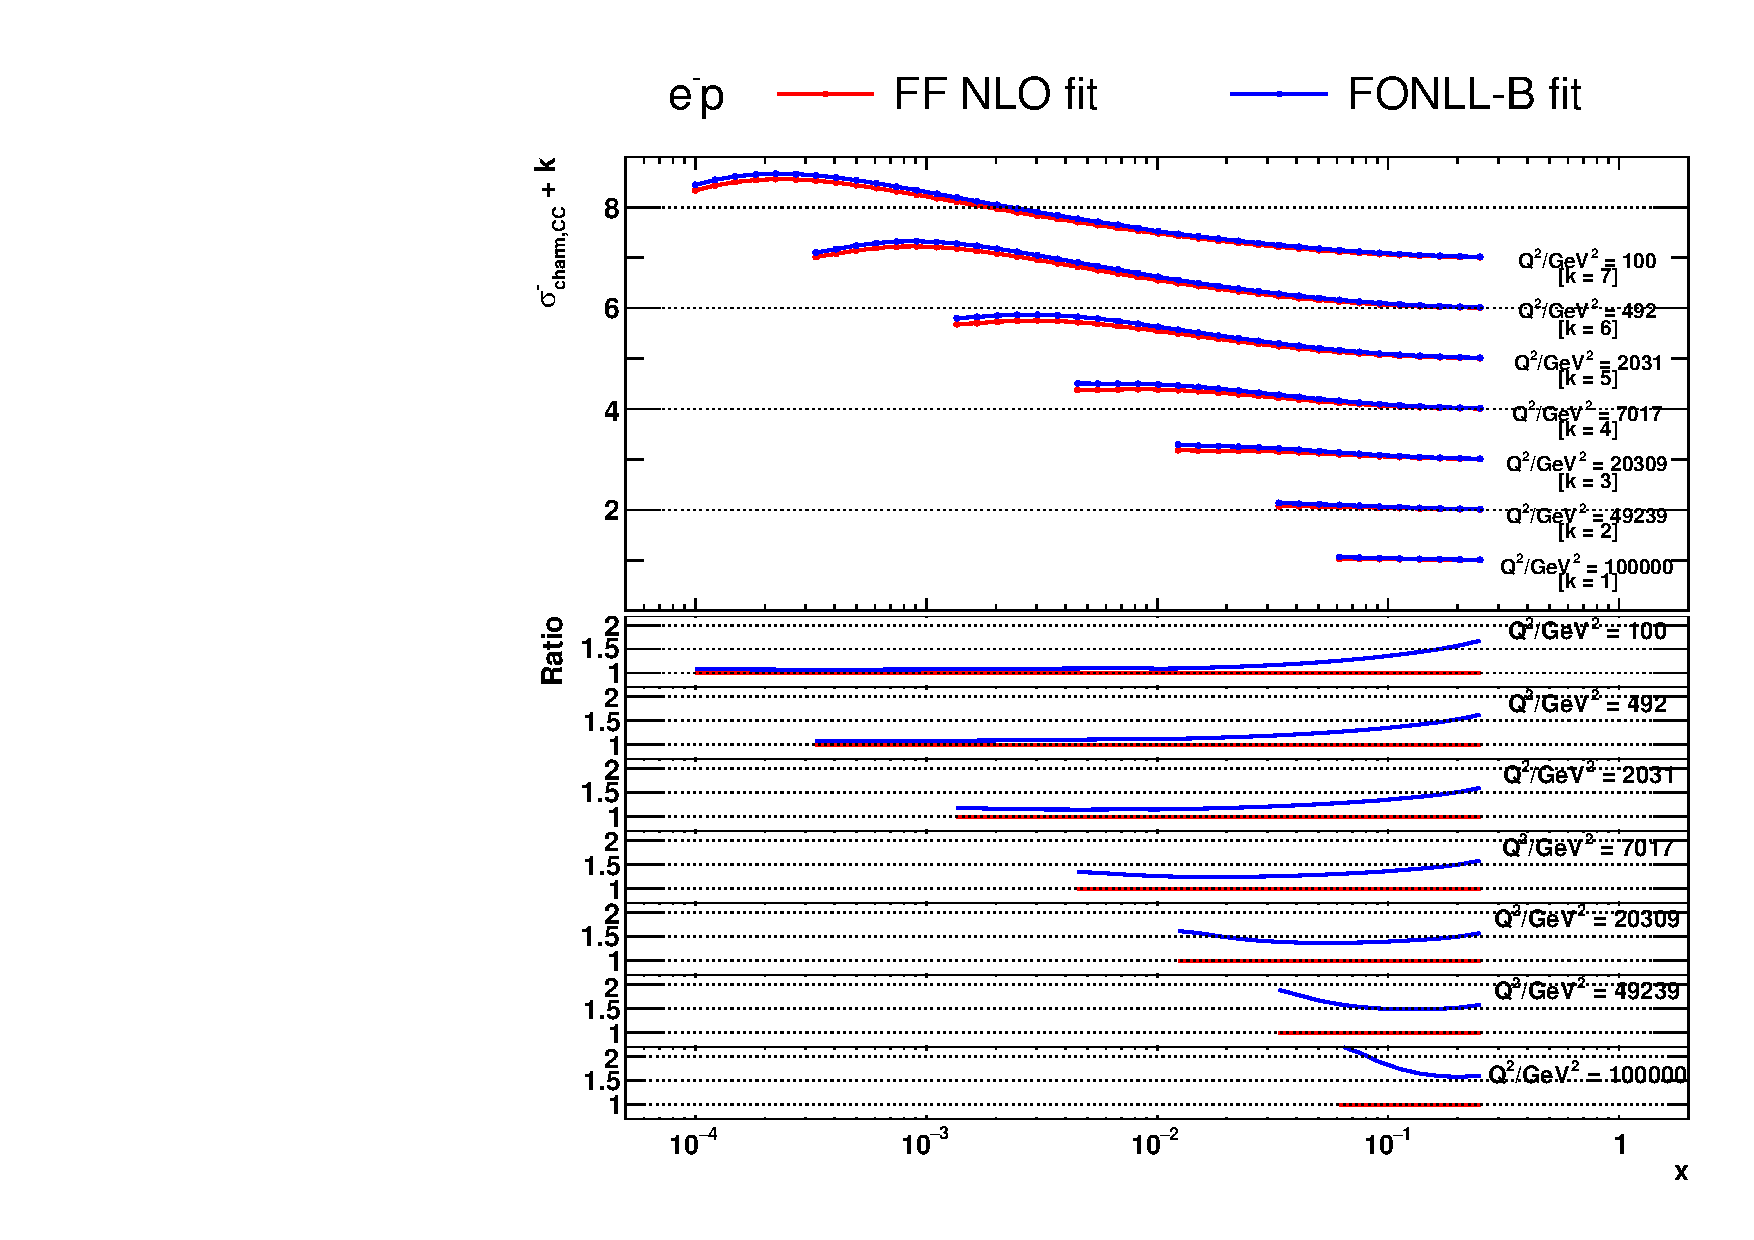
\includegraphics[width=0.49\textwidth]{pics/plots-191018/plot-fit-x-em.pdf}}}
%    \centering{{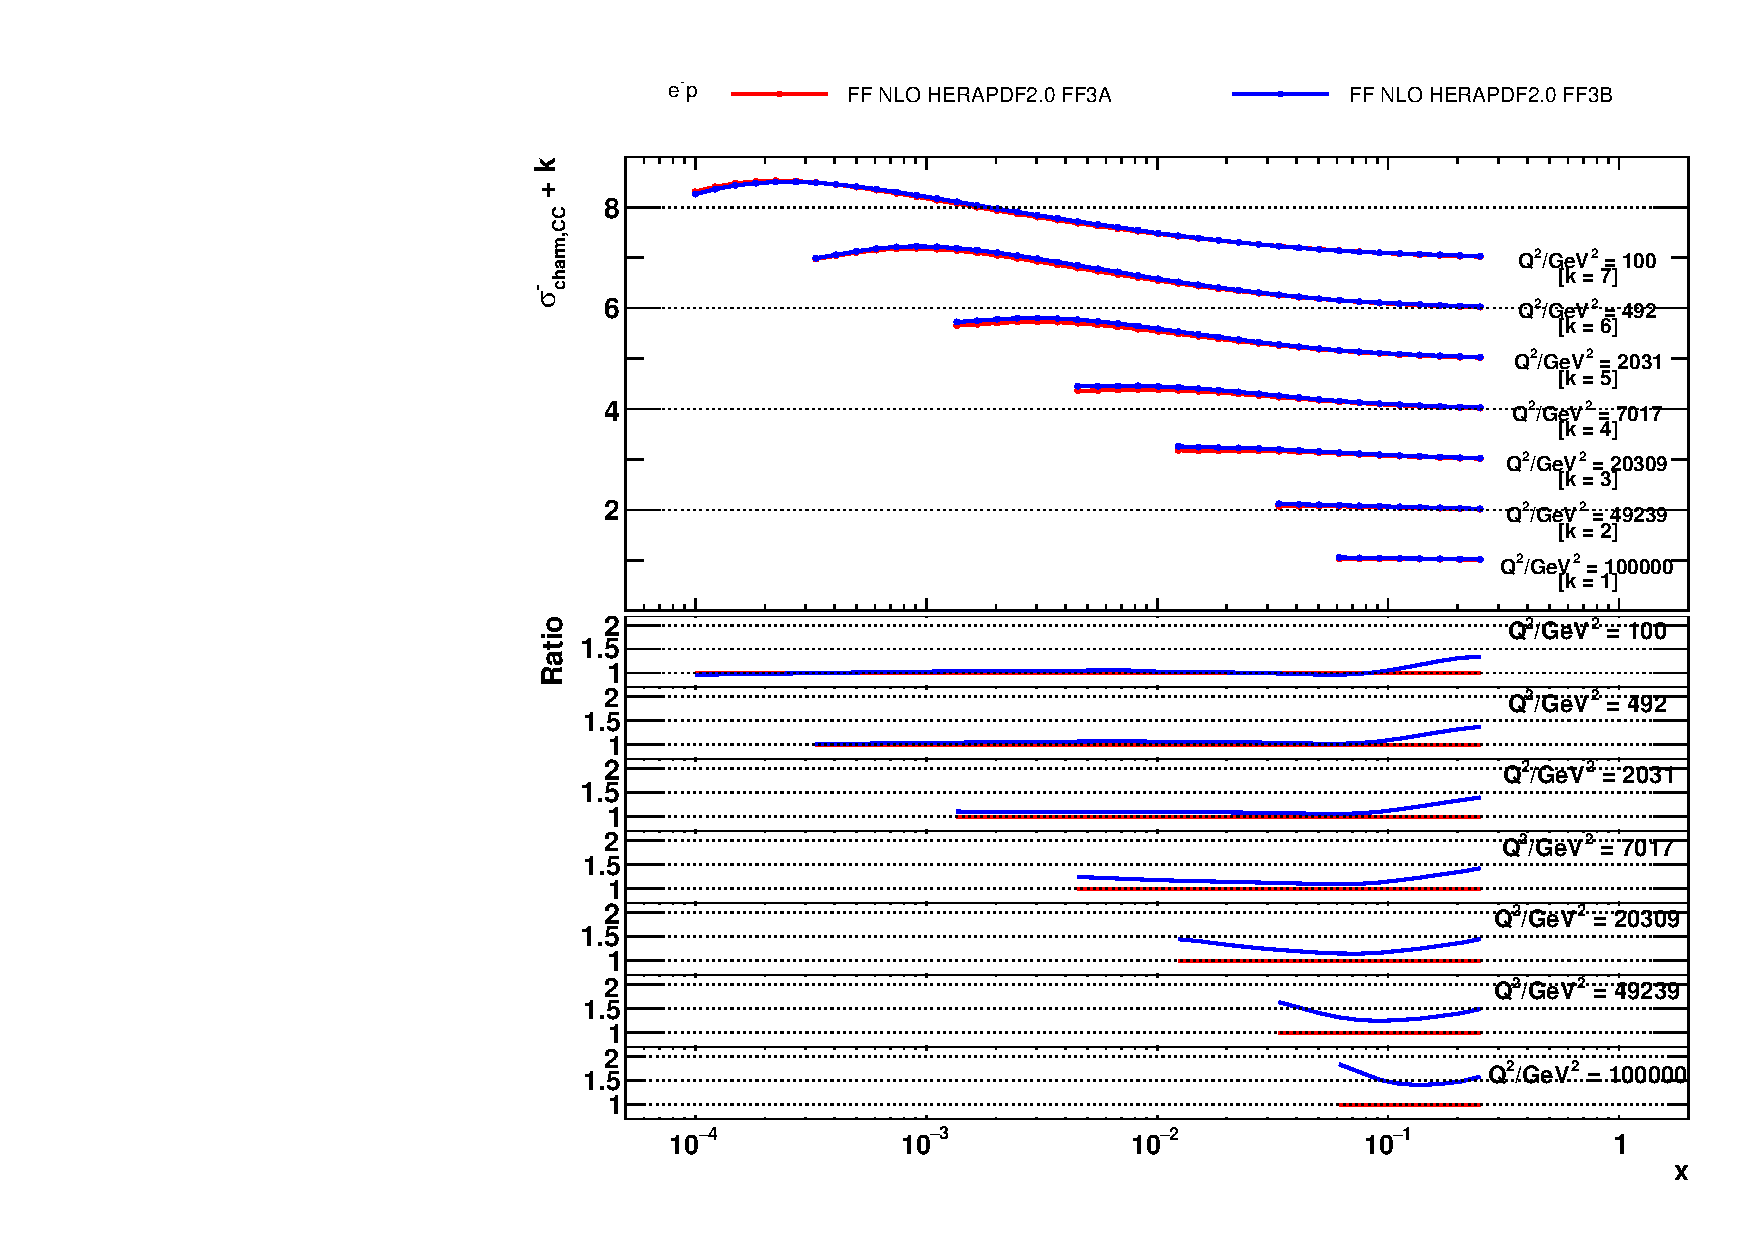
\includegraphics[width=0.49\textwidth]{pics/plots-191018/plot-FF3AB-x-em.pdf}}}
%    \caption{(left) The theoretical predictions for charm CC production at the LHeC as a function of $Q^2$ for different values of $\xbj$. See Fig.~\ref{fig:thpred-fit-y} for further details.}
%    \label{fig:thpred-fit-x}
%\end{figure*}
%
%\begin{figure*}
%    \centering
%    \centering{{\includegraphics[width=0.49\textwidth]{pics/plots-191018/plot-FF3ABFONLL-y-em.pdf}}}
%    \centering{{\includegraphics[width=0.49\textwidth]{pics/plots-191018/plot-FF3ABFONLL-y-em.pdf}}}\\
%    \centering{{\includegraphics[width=0.49\textwidth]{pics/plots-191018/plot-FF3ABFONLL-y-em.pdf}}}
%    \caption{The theoretical predictions for charm CC production at the LHeC as a function of $y$ for different values of $Q^2$ obtained in the fit to the HERA data in the \ffns and \fonll schemes. The bottom panel display the theoretical predictions normalized to the nominal values of the \ffns predictions. (right) Same predictions but obtained in the \ffns and \ffnsb schemes using the \ffthreea and \ffthreeb sets, respectively. The bottom panel display the theoretical predictions normalized to the nominal values of the \ffnsb predictions.}
%    \label{fig:thpred-fit-y}
%\end{figure*}

\begin{figure}
  \centering
  \centering{{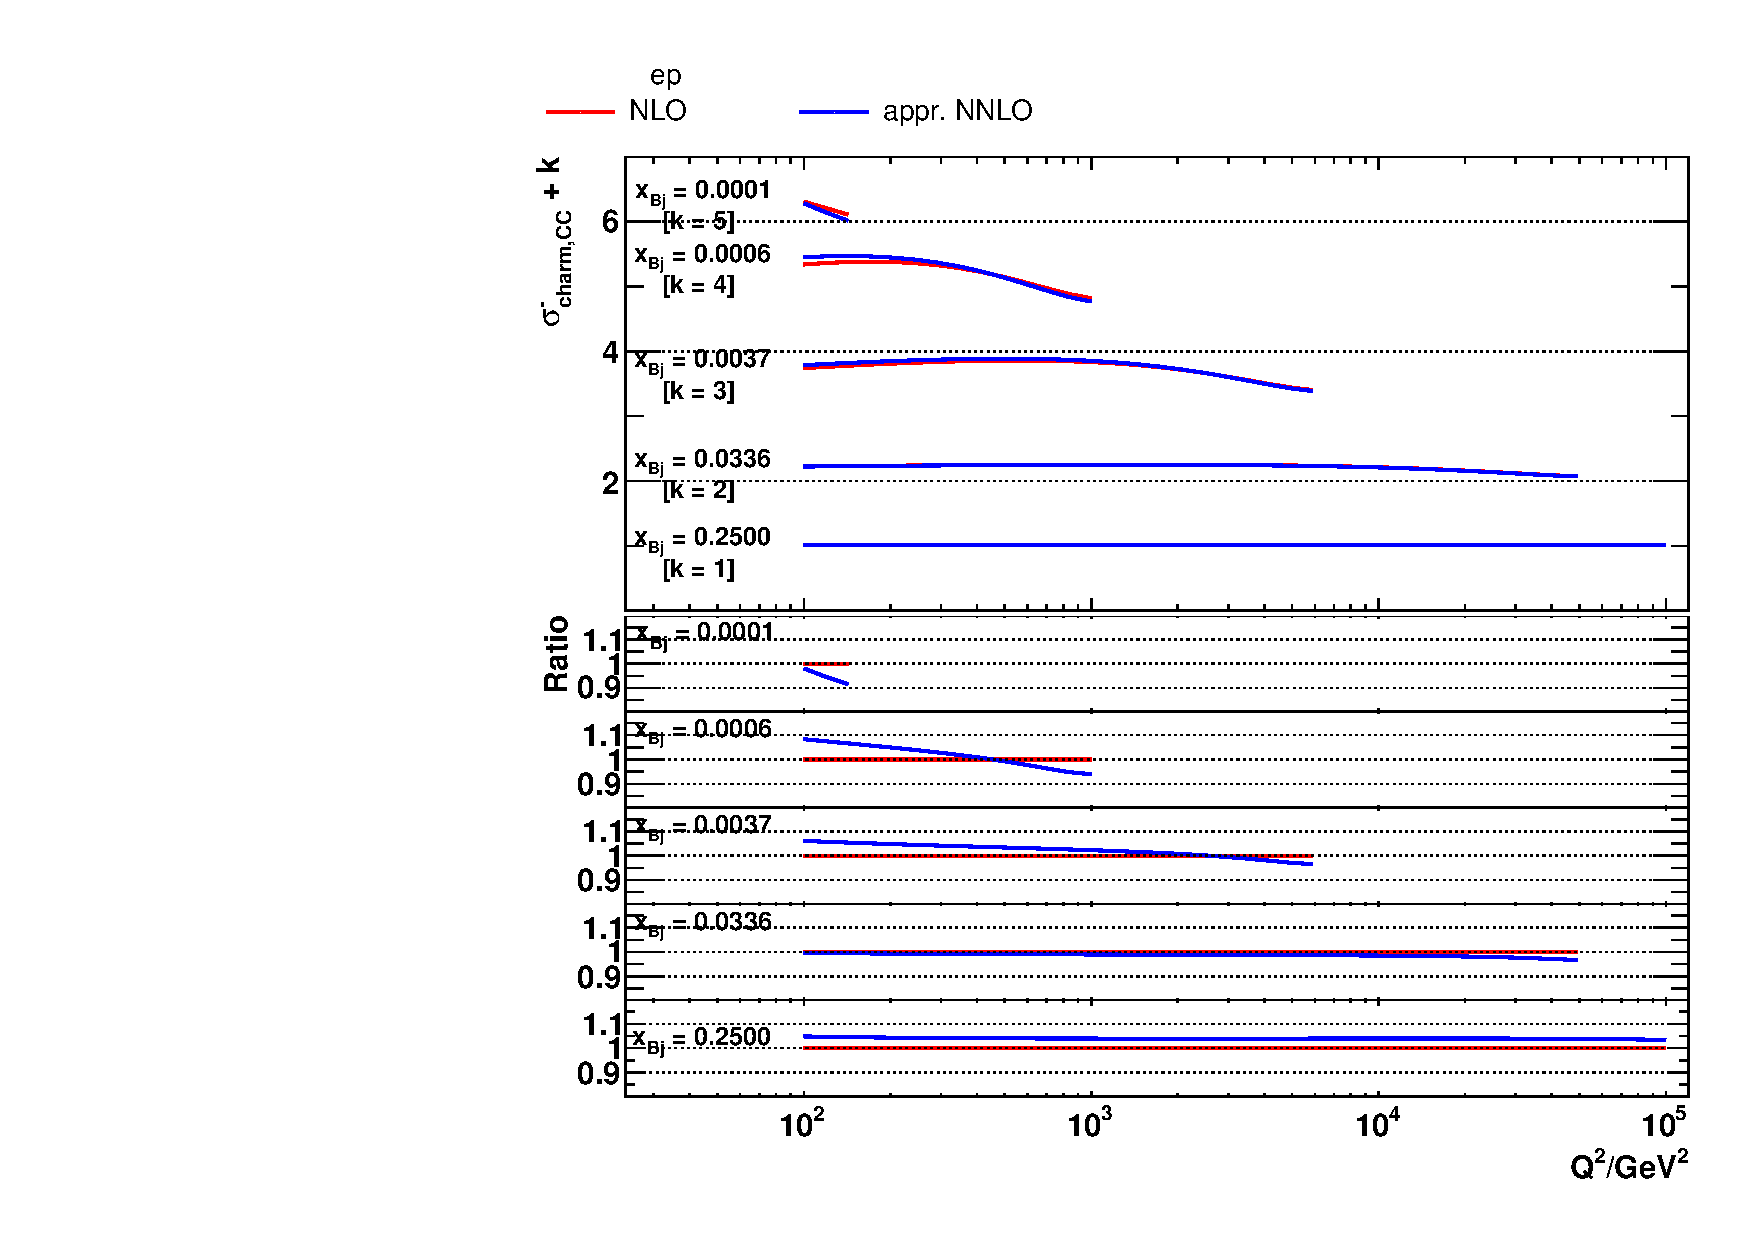
\includegraphics[width=0.50\textwidth]{pics/final/plot-FFABMnnlo-q2-em.pdf}}}
  \caption{The theoretical predictions
    for CC charm production at the LHeC as a function of $Q^2$ for
    different values of \xbj calculated in the \ffns scheme at NLO and
    approximate NNLO. The bottom panels display the theoretical
    predictions normalized to the nominal values of the \ffns NLO
    predictions.}
  \label{fig:thpred-q2-nnlo}
\end{figure}


%\color{blue} %%%%%%%%%%%%%%%%%%%%%%%%%%%%%%%%%%%
%
To better understand the differences between the FFNS and VFNS
calculations, Fig.~\ref{fig:thpred-ff3abfonll} is particularly
instructive.
%
We see that at low $Q^2$ the FFNS (\ffns and \ffnsb) and VFNS
(\fonll) results agree within uncertainties (as demonstrated in 
Fig.~\ref{fig:thpred-q2}). When the scale $\mu$ is
below the charm-threshold scale $\mu_c$ (typically taken to be equal
to $m_c(m_c)$) the charm PDFs vanish and the FFNS and VFNS reduce to
the same result.\footnote{Note that while the charm-threshold scale
  $\mu_c$ is commonly set to the charm quark mass $m_c(m_c)$, the
  choice of $\mu_c$ is arbitrary and amounts to a renormalization
  scheme choice~\cite{Bertone:2017ehk}.}
%
For increasing scales, the VFNS resums the $\alpha_s\ln(\mu^2/\mu_c^2)$
contributions via the DGLAP evolution equations and the FFNS and VFNS
will slowly diverge logarithmically. This behavior is observed in
\hbox{Fig.~\ref{fig:thpred-ff3abfonll}} and is consistent with the
characteristics demonstrated in Ref.~\cite{Kusina:2013slm}.

More precisely, Ref.~\cite{Kusina:2013slm} used a matched set of
$n_f=3$ and $n_f=5$ PDFs to study the impact of the scheme choice at
large scales. They found that the resummed contributions in the VFNS
yielded a larger cross section than the FFNS (the specific magnitude
was $x$-dependent), and that for $Q^2$ scales more than a few times
the quark mass, the differences due to scheme choice exceeded the
differences due to (estimated) higher-order
contributions.
%
Thus, we have identified the source of the scheme differences at large $Q^2$.

%\textcolor{blue}{
The  source of the scheme differences at large $\xbj$ is a bit more subtle. 
The VFNS includes a resummation of higher-order logarithms of the form $\alpha_s \ln(\mu^2/\mu_c^2 )$.
In Fig.~\ref{fig:acot} of the Appendix we display the separate contributions of the VFNS for a choice of
$\{\xbj,Q^2\}$; the difference  between the LO and SUB curves is indicative of the
additional contribution of the resummed logarithms.
This contribution depends on the particular $\xbj$ value and we find
({\it c.f.,} Fig.~11 of Ref.~\cite{Kusina:2013slm})
that these terms increase for larger $\xbj$ values. 
%
Figure~\ref{fig:thpred-ff3abfonll} indicates that a large fraction of these seems to be caught by the \ffnsb scheme.
%
Thus, we have identified the source of the scheme differences at large $\xbj$.
%}



%%%%%%%%%%%%%%%%%%%%%%%%%%%%%%%%%%%%%%%%%
\subsection{Contributions from different partonic subprocesses}
\label{sec:thpred-partonic}

%\textcolor{red}{NEED TO COMMENT ABOUT THE GLUON AT NLO}

The fundamental difference between the FFNS and the VFNS is the
treatment of the heavy partons, the charm in particular. In the FFNS
the charm is not included in the PDFs as an active parton, so charm
quarks only arise from gluon splitting, $g\to c \bar{c}$. In contrast,
the VFNS does include the charm as an active partonic flavor, and thus
allows for charm-initiated subprocesses.
%
To better appreciate these differences, we will study the individual
partonic contributions to the cross section as functions of the
kinematic variables \xbj, $Q^2$, and $y$.

Figs.~\ref{fig:partonic-x}, \ref{fig:partonic-q2}
and~\ref{fig:partonic-y} show the contributions from separate partonic
subprocesses to the CC charm production cross section in the \ffns and
\fonll schemes as a function of: \xbj for different values of $Q^2$,
$Q^2$ for different values of \xbj, and $y$ for different values of
$Q^2$, respectively.

%\color{blue} %%%%%%%%%%%%%%%%%%%%%%%%%%%%%%%%%%%
%
In these figures we observe that the gluon contribution to the FFNS is
strikingly similar to the charm contribution to the VFNS.
%
This is explained by the fact that in the FFNS the charm is present
only in the final state and produced predominantly in the hard process
$\gamma g \to c\bar{c}$. In contrast, in the VFNS the charm is present also
in the initial state and mainly produced by $g\to c\bar{c}$ collinear
splitting through DGLAP evolution.
%
The fundamental underlying process is (and has to be) the same in both
the FFNS and VFNS, but the factorization boundary between PDFs and
hard scattering cross section, $\hat{\sigma}\otimes f$, (determined by
the scale $\mu$ and the scheme choice) is different.\footnote{Note
  there is a ``subtraction'' term which closely matches the LO
  process, but this ${\cal O}(\alpha_s)$ process is contained in the
  NLO gluon-initiated contribution.  For details,
  see~\ref{sec:appendix} }


These figures highlight another interesting feature of the QCD theory;
we observe that for the VFNS the gluon contribution (green curves) can
become negative in particular kinematic regions.
This is because in the VFNS we combine the gluon-boson fusion process
(the NLO terms of Figs.~\ref{fig:tchannel} and~\ref{fig:uchannel})
with the counter-term  (the SUB terms),
and this combination can be negative.
%
This behavior underscores the fact that the renormalization scale $\mu$
is simply ``shuffling'' contributions among the separate sub-pieces,
but the total physical cross section remains positive and stable,
{\it cf.}, Fig.~\ref{fig:acot} and Ref.~\cite{Aivazis:1993pi}.
This is a triumph of the QCD theory. 


%\color{black} %%%%%%%%%%%%%%%%%%%%%%%%%%%%%%%%%%%

Next, turning our attention to the strange PDF contribution, it is
notable that the FFNS and VFNS behave qualitatively very similar as
functions of $Q^2$, \xbj, and $y$. In particular, we observe that the
strange fraction increases for \xbj and decreases for $Q^2$ and $y$.
%
In particular, at high $y$ the strange PDF contribution drops to zero
in favor of the gluon or charm quark PDFs (see
Fig.~\ref{fig:partonic-y} and Eq.~(\ref{eq:y01})). Similar phenomena
(although less pronounced) are observed at low \xbj and/or high
$Q^2$. In these phase-space regions, the dominant contributions to the
cross section are proportional to the gluon PDF in the FFNS or to the
charm-quark PDFs in the VFNS.

\begin{figure*}
  \centering
  \centering{{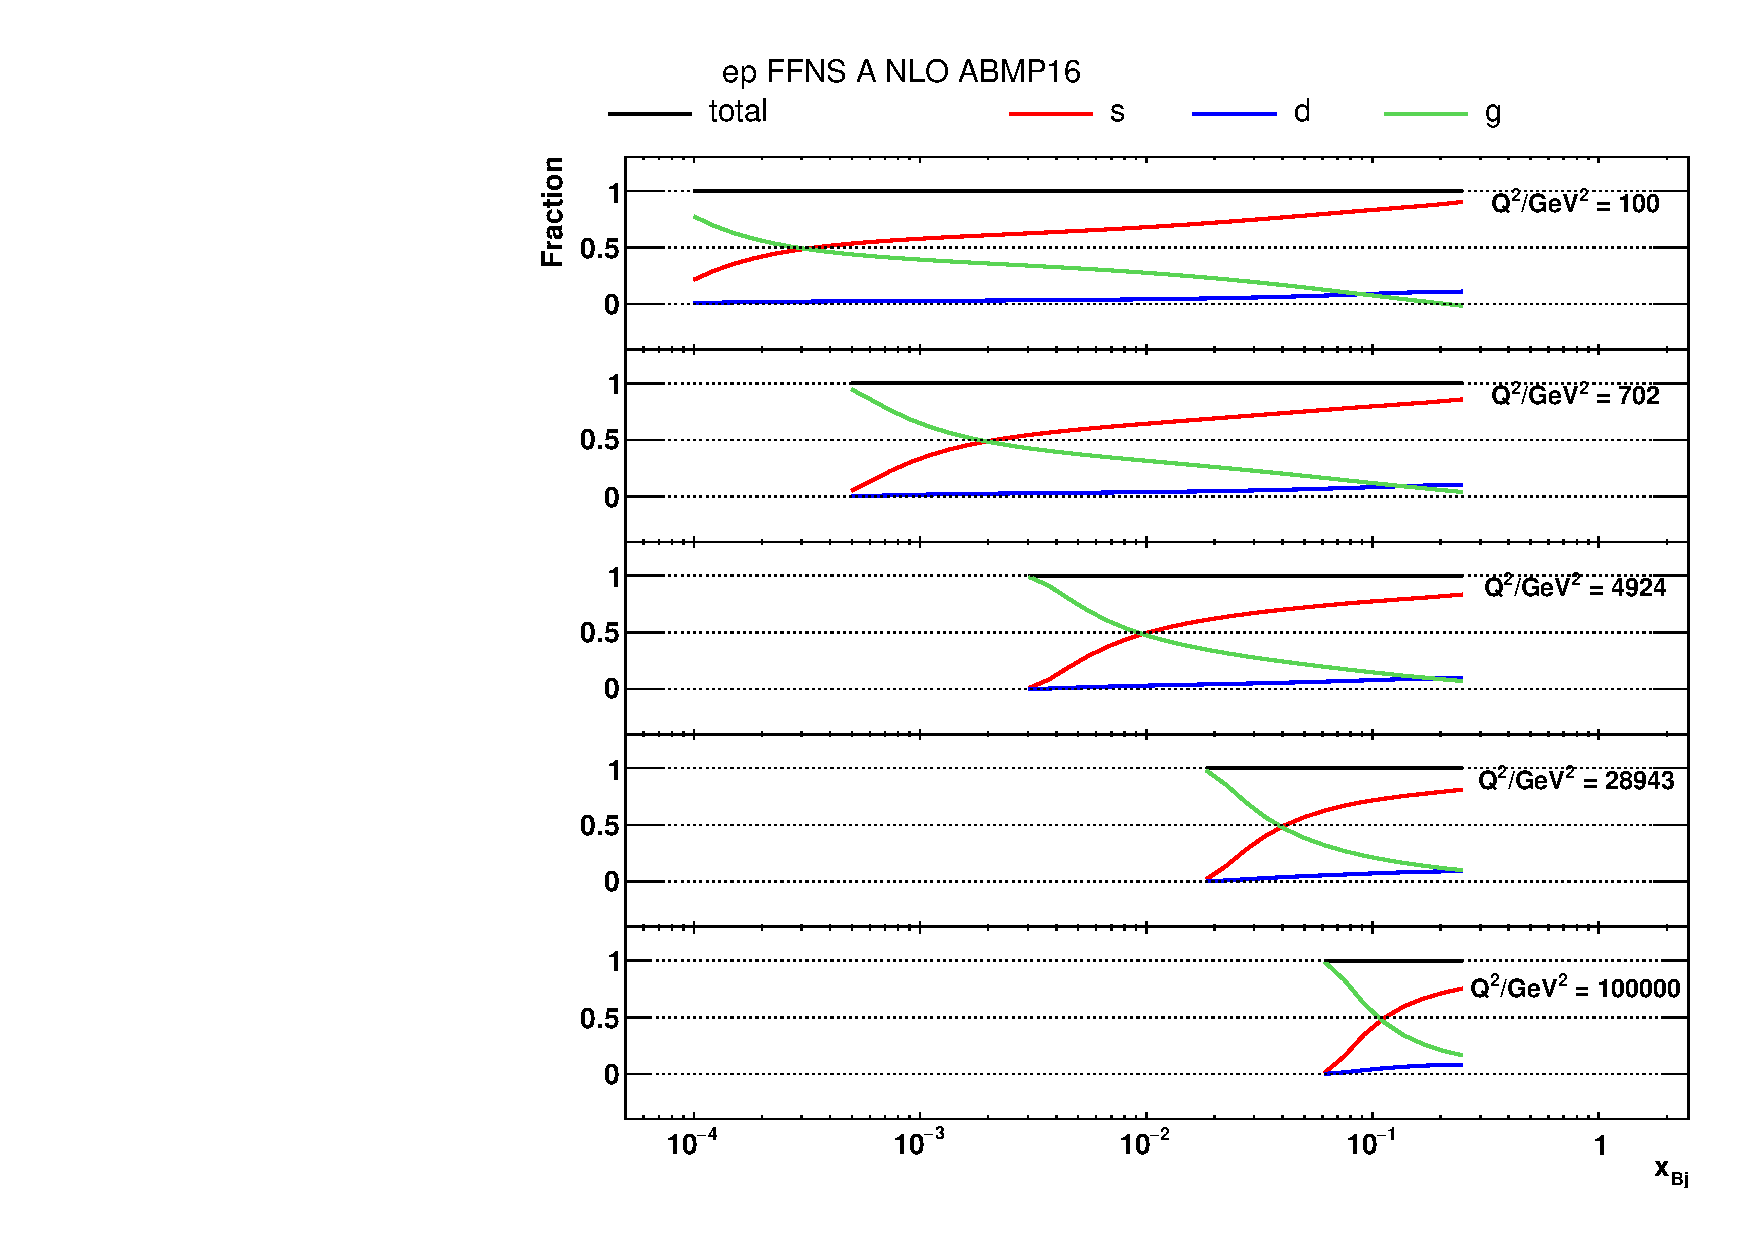
\includegraphics[width=0.49\textwidth]{pics/final/plot-parton-x-em-FFABM.pdf}}}
  \centering{{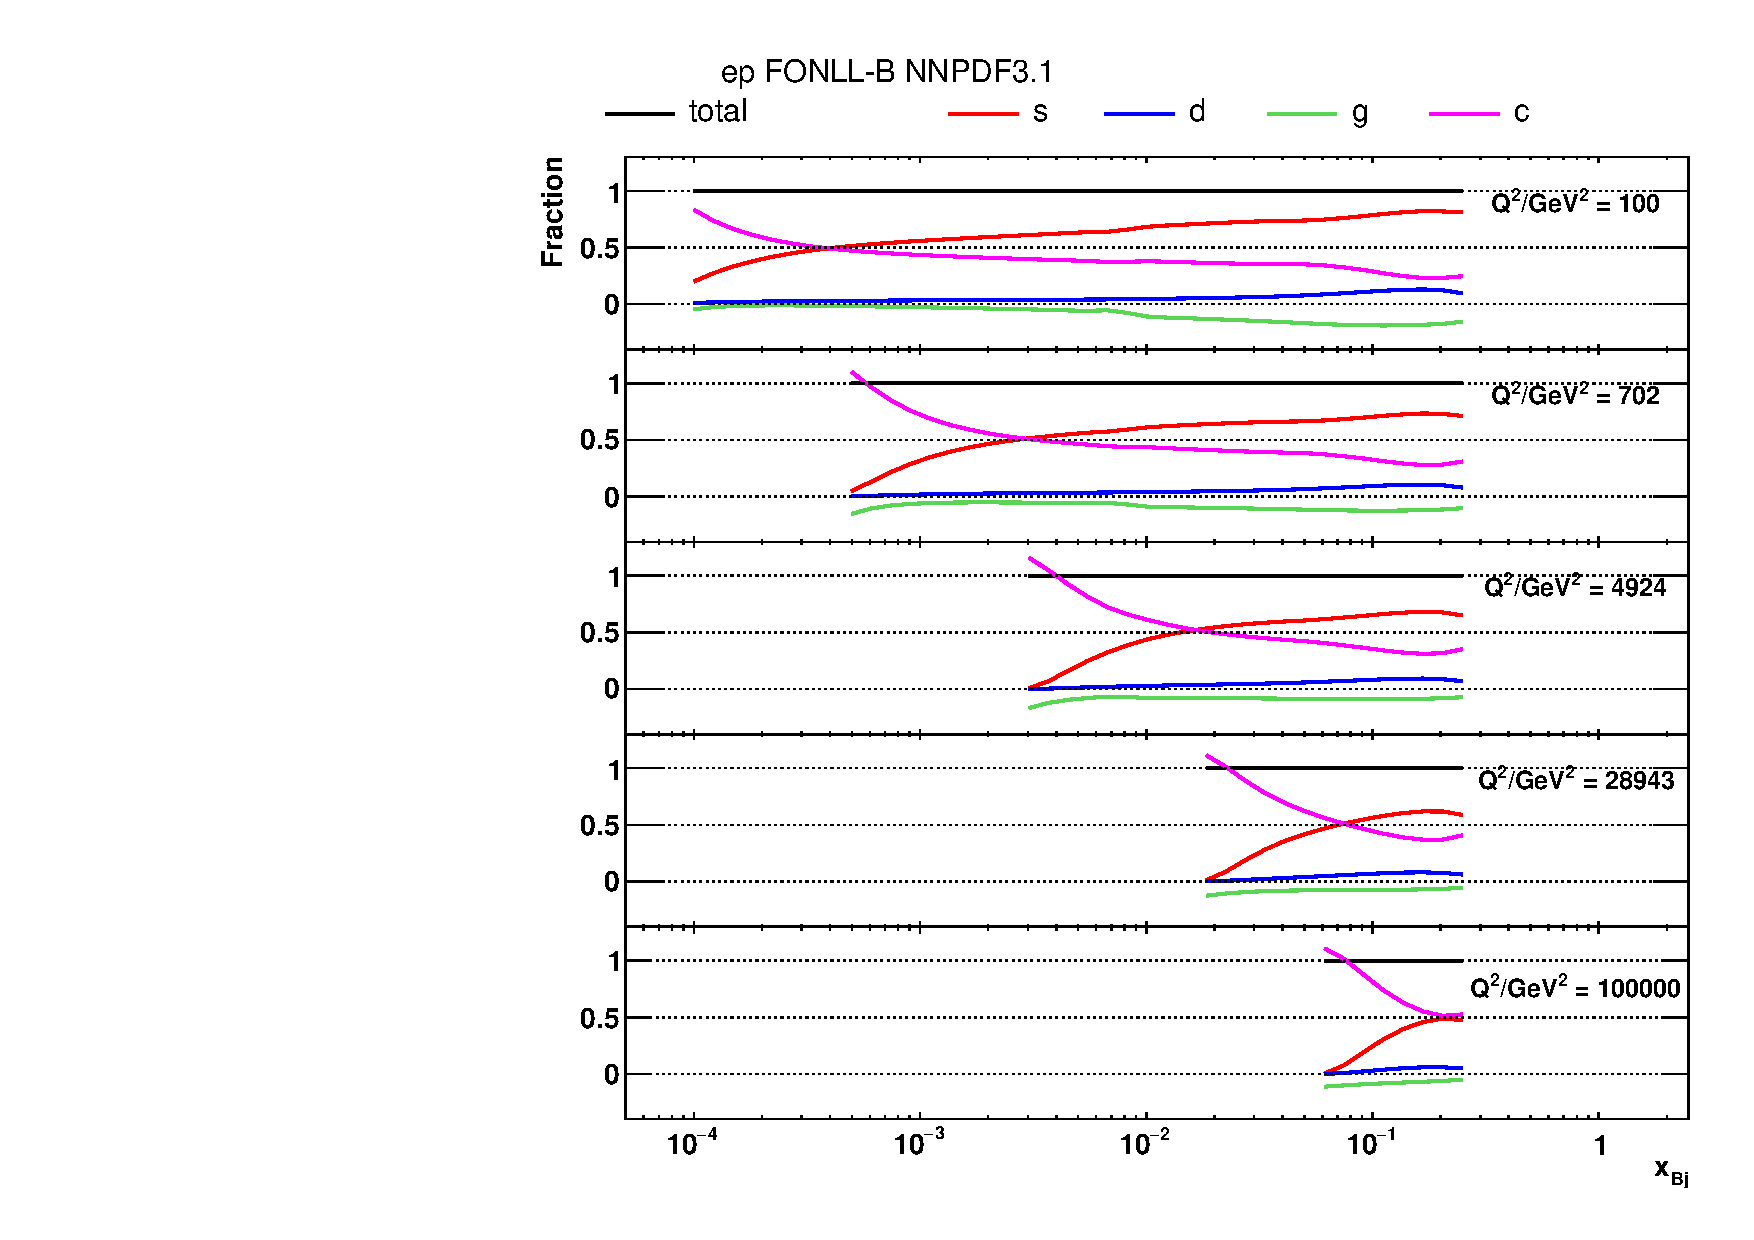
\includegraphics[width=0.49\textwidth]{pics/final/plot-parton-x-em-FONLL.pdf}}}
  \caption{The partonic subprocesses for charm CC production cross
    sections in the \ffns (left) and \fonll (right) schemes as a
    function of \xbj for different values of $Q^2$.}
  \label{fig:partonic-x}
\end{figure*}

\begin{figure*}
  \centering
  \centering{{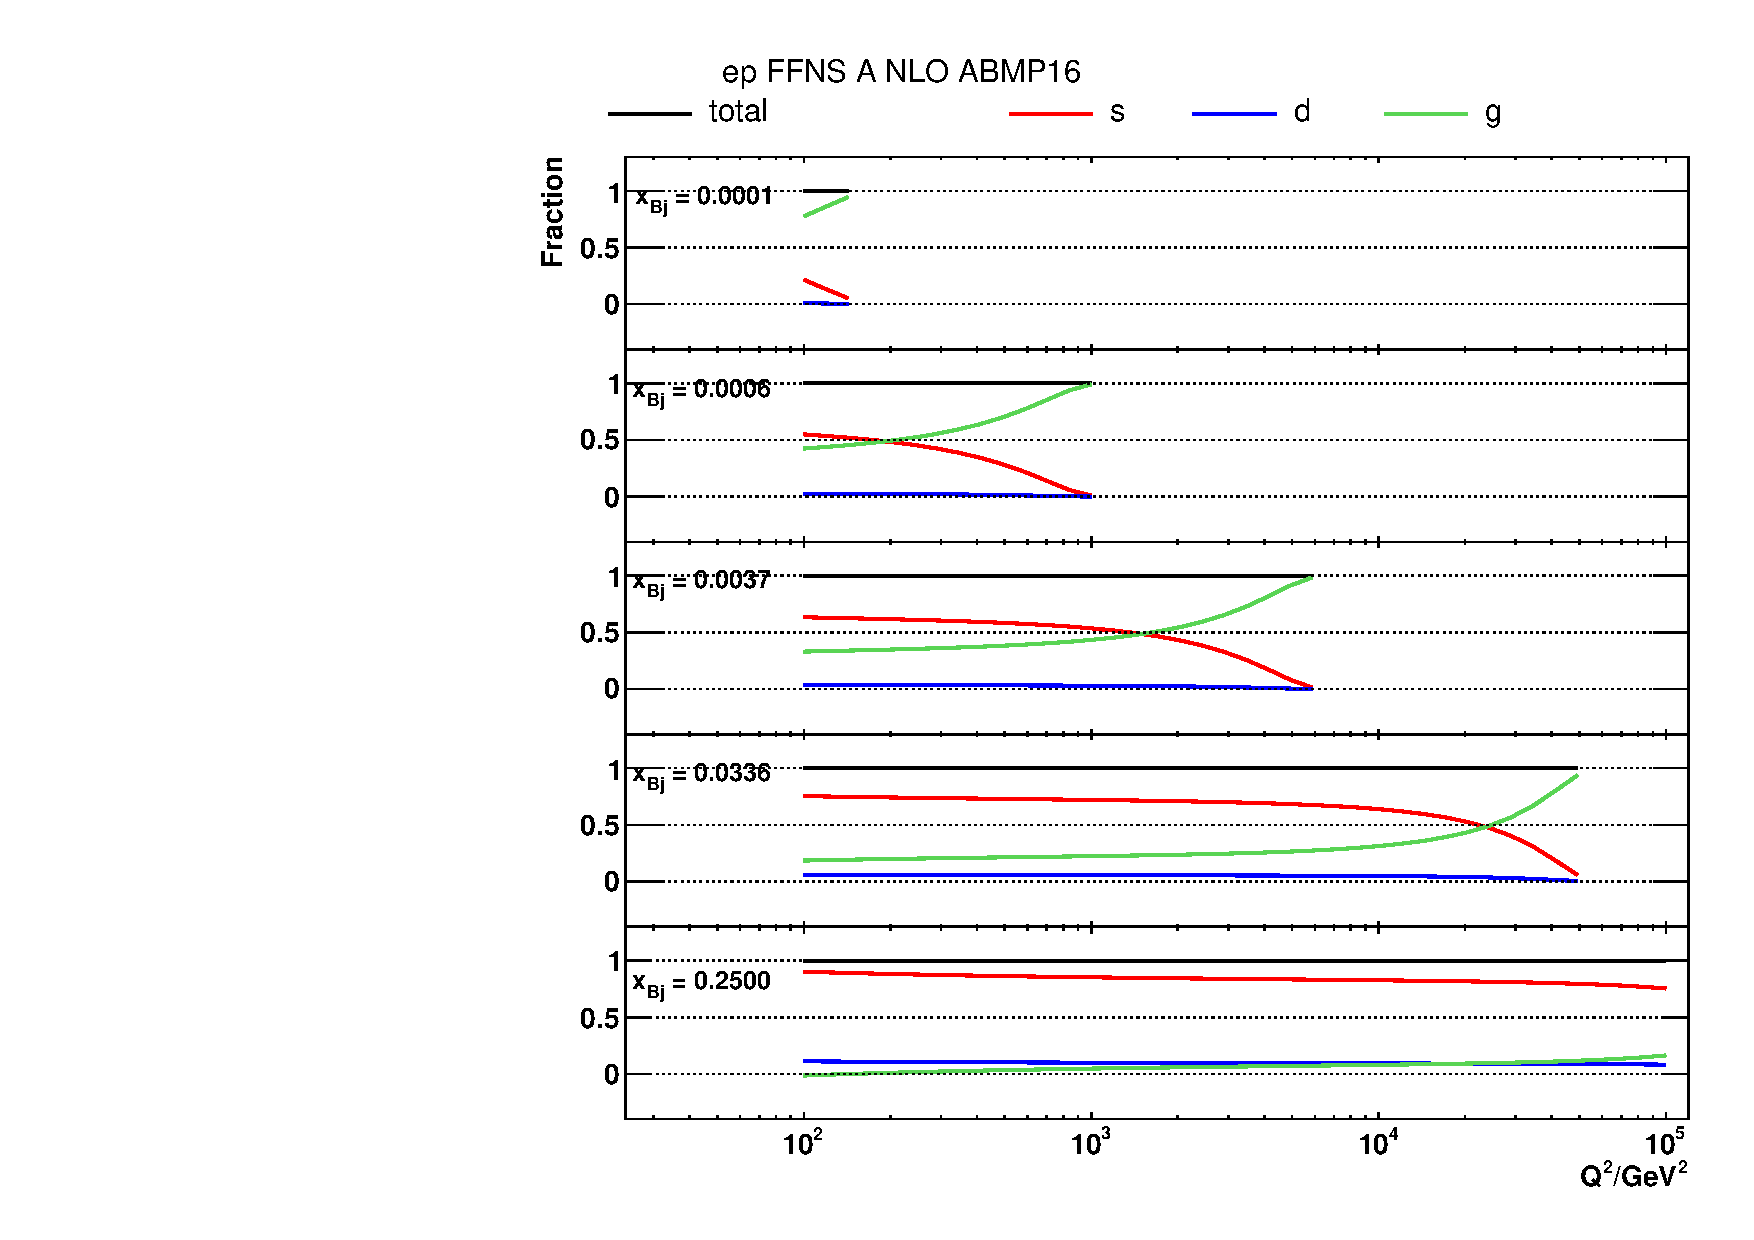
\includegraphics[width=0.49\textwidth]{pics/final/plot-parton-q2-em-FFABM.pdf}}}
  \centering{{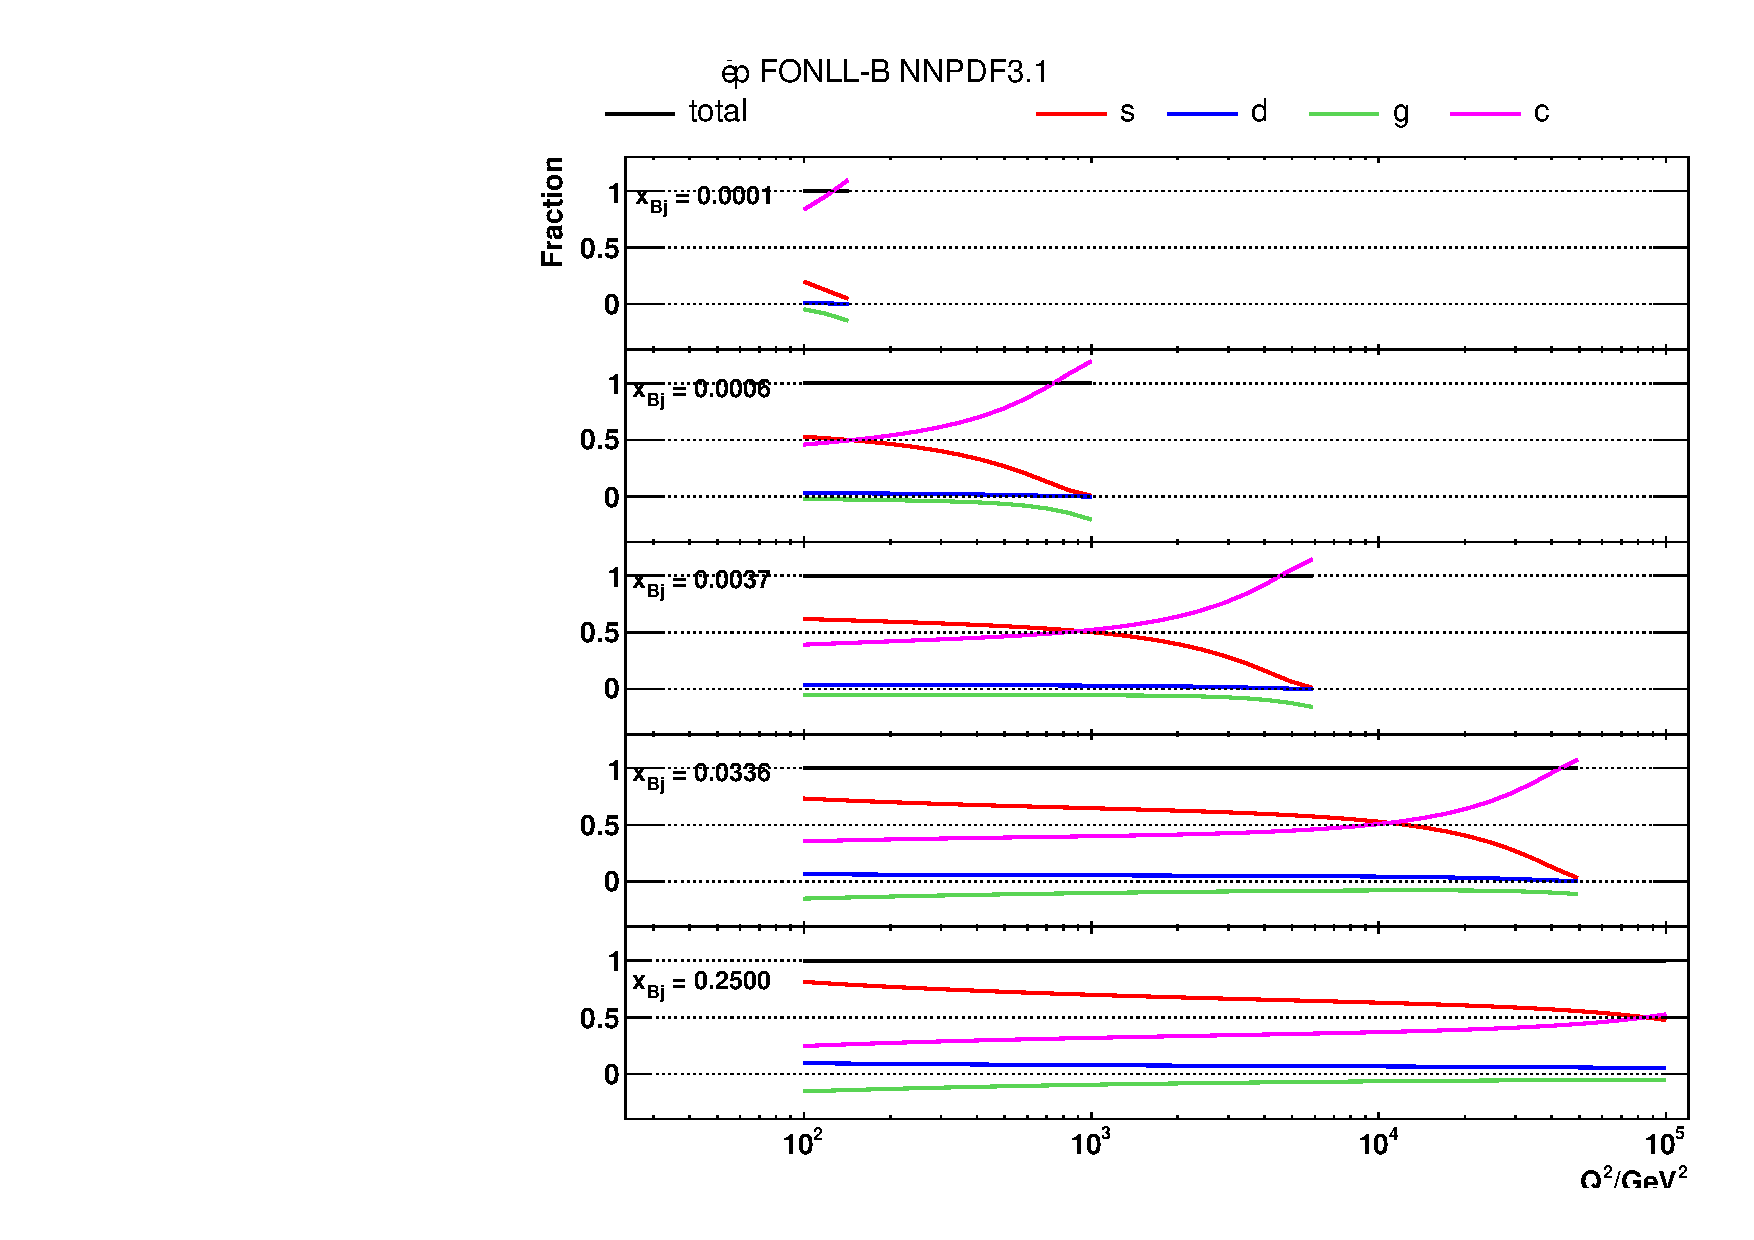
\includegraphics[width=0.49\textwidth]{pics/final/plot-parton-q2-em-FONLL.pdf}}}
  \caption{The partonic subprocesses for charm CC production cross
    sections in the \ffns (left) and \fonll (right) schemes as a
    function of $Q^2$ for different values of \xbj.}
  \label{fig:partonic-q2}
\end{figure*}

\begin{figure*}
  \centering
  \centering{{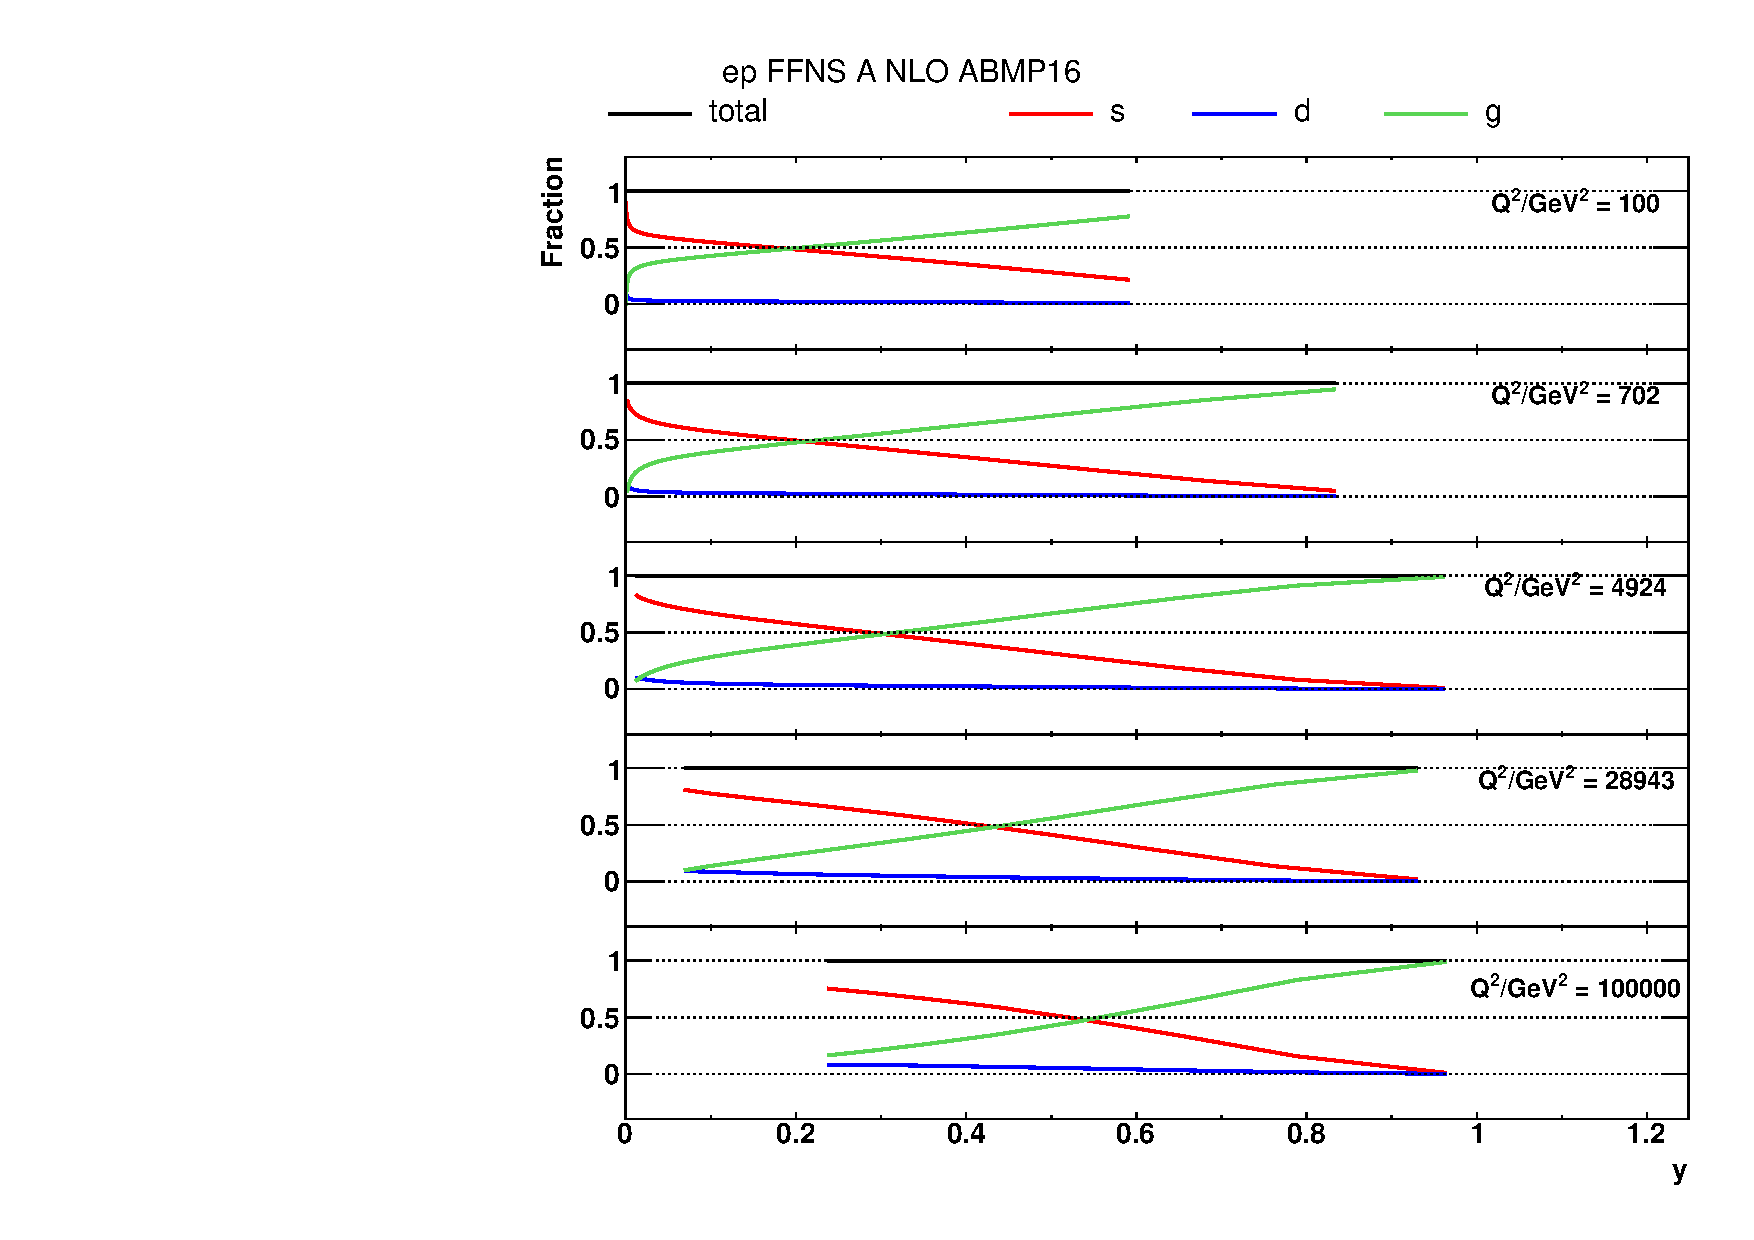
\includegraphics[width=0.49\textwidth]{pics/final/plot-parton-y-em-FFABM.pdf}}}
  \centering{{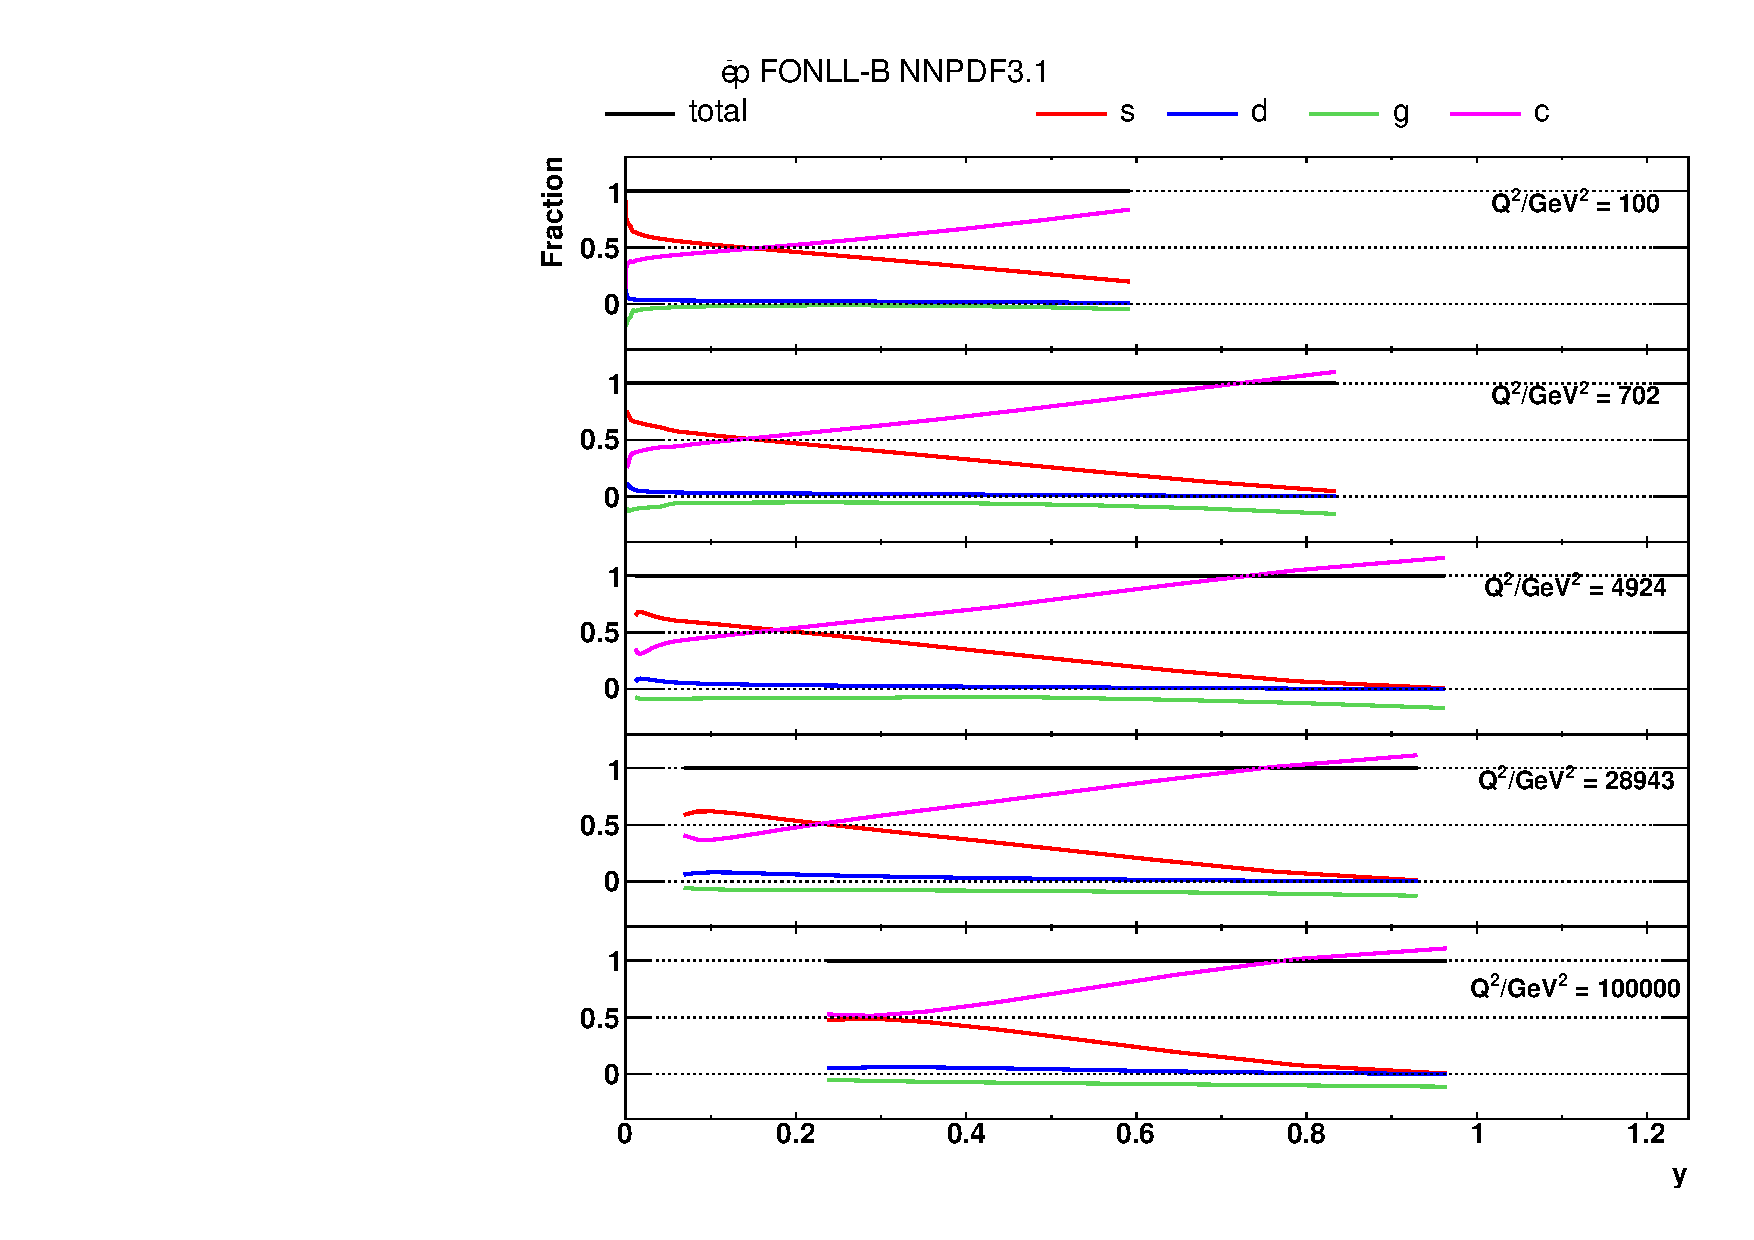
\includegraphics[width=0.49\textwidth]{pics/final/plot-parton-y-em-FONLL.pdf}}}
  \caption{The partonic subprocesses for charm CC production cross
    sections in the \ffns (left) and \fonll (right) schemes as a
    function of $y$ for different values of $Q^2$.}
  \label{fig:partonic-y}
\end{figure*}

%%%%%%%%%%%%%%%%%%%%%%%%%%%%%%%%%%%%%%%%%%%%%%%%%%%%%
\section{PDF constraints from charm CC pseudodata}
\label{sec:PDF}

Now we turn to examine how the LHeC can reduce the PDF uncertainties
and thus improve our predictive power.

The impact of charm CC cross section measurements at the LHeC on the
PDFs is quantitatively estimated using the profiling
technique~\cite{Paukkunen:2014zia}. This technique is based on
minimizing the \chisq between data and theoretical predictions taking
into account both experimental and theoretical uncertainties arising
from PDF variations.
%
Two NLO PDF sets were chosen for this study:
\abmp~\cite{Alekhin:2018pai} and \nnpdf~\cite{Ball:2017nwa}. All PDF sets are provided with
uncertainties in the format of eigenvectors.

%%%%%%%%%%%%%%%%%%%%%%%%%%%%%%%%%%%%%%%%%%%%%%%%%%%%%
\subsection{The CC  charm pseudodata}
\label{sec:pseudodata}

For this study, pseudodata for charm CC production cross section
differential in $Q^2$ and \xbj and corresponding to an integrated
luminosity of $100{\rm~fb}^{-1}$~\cite{AbelleiraFernandez:2012cc,Blumlein:1992we} and
polarization $P=-0.8$ are used.
%
%\textcolor{red}{\bf [TODO: describe how pseudodata were produced]}
%
Theoretical predictions are calculated at NLO
in pQCD both in the \ffns with number of active flavors $n_f = 3$ and
in the \fonll scheme. The charm-mass reference value in the
$\overline{\mbox{MS}}$ scheme is set to $m_c(m_c) = 1.27$ GeV and
$\alpha_s$ is set to the value used for the corresponding PDF
extraction. The renormalization and factorization scales are chosen to
be $\mu_\mathrm{r}^2 = \mu_\mathrm{f}^2 = Q^2$.

The \chisq value is calculated as follows:
\begin{equation}
\begin{split}
  \chisq = \mathbf{R}^{T}_{} \mathbf{Cov}^{-1}_{} \mathbf{R}_{} + \sum_{\beta} b_{\beta,\rm th}^2 \ , \\[5pt]
  \mathbf{R} = \mathbf{D} - \mathbf{T} - \sum_{\beta} \Gamma^{}_{\beta,\rm th} b_{\beta,\rm th} \ ,
\label{eq:chisq}
\end{split}
\end{equation}
%
where $\mathbf{D}$ and $\mathbf{T}$ are the column vectors of the
measured (data) and predicted (theory) values, respectively.  The
correlated theoretical PDF uncertainties are included using the
nuisance parameters $b_{\beta, \rm th}$ with their influence on the
theory predictions described by $\Gamma_{\beta,\rm th}$, where the
index $\beta$ runs over all PDF eigenvectors. For each nuisance
parameter a penalty term is added to the \chisq, representing the
prior knowledge of the parameter. No theoretical uncertainties except
the PDF uncertainties are considered. The full covariance matrix ${\bf Cov }$
representing the statistical and systematic uncertainties of the data
is used in the fit. The statistical and systematic uncertainties are
treated as additive, \textit{i.e.} they do not change in the fit. The
systematic uncertainties are assumed uncorrelated between bins.

To treat the asymmetric PDF uncertainties of the \nnpdf set, the
\chisq function in Eq.~(\ref{eq:chisq}) is generalized assuming a
parabolic dependence of the prediction on the nuisance
parameters~\cite{Alekhin:2014irh}:
\begin{eqnarray}
\Gamma^{}_{\beta, \rm th} \to \Gamma^{}_{\beta, \rm th} +  \Omega^{}_{\beta, \rm th}b_{\beta, \rm th}\,, \label{eq:iter}
\end{eqnarray}
where
$\Gamma^{}_{\beta, \rm th} = \frac12(\Gamma^{+}_{\beta, \rm th} -
\Gamma^{-}_{\beta, \rm th})$
and
$\Omega^{}_{\beta} = \frac12 (\Gamma^{+}_{\beta, \rm th} +
\Gamma^{-}_{\beta, \rm th})$
are determined from the shifts of the predictions corresponding to up
($\Gamma^{+}_{\beta, \rm th}$) and down
($ \Gamma^{-}_{\beta, \rm th}$) variations of each PDF eigenvector.

The values of the nuisance parameters at the minimum,
$b^{\rm min}_{\beta,\rm th}$, are interpreted as optimized, or
profiled, PDFs, while  uncertainties of $b^{\rm min}_{\beta,\rm th}$   determined using the
tolerance criterion of $\Delta\chi^2 = 1$ correspond to the new PDF
uncertainties. The profiling approach assumes that the new data are
compatible with the theoretical predictions using the existing PDFs,
such that no modification of the PDF fitting procedure is
needed. Under this assumption, the central values of the measured
cross sections are set to the central values of the theoretical
predictions.


%%%%%%%%%%%%%%%%%%%%%%%%%%%%%%%%%%%%%%%%%%%%%%%%%%%%%
\subsection{The profiled PDFs}
\label{sec:profile}

\new{
The profiling study is performed using two sets of LHeC charm CC pseudodata:
\begin{itemize}
 \item the full set,
 \item a restricted set with data points for which the difference between the \ffns and \fonll are smaller than the present PDF uncertainties. 
 The latter is taken for simplicity as the sum of the \abmp and \nnpdf uncertainties, but for the most data points it is dominated by the \nnpdf uncertainties (see Fig.~\ref{fig:thpred-q2-unc}).
\end{itemize}
Given the sizable differences observed between the \ffns and \fonll predictions, the study with the restricted data set (also referred to as `with cuts') aims to check whether or not model independent constraints on the strange PDF can be extracted using the charm CC reaction at LHeC. The two sets of data points are shown in Fig.~\ref{fig:data} as functions of $Q^2$ and \xbj.
}

The original and profiled \abmp and \nnpdf PDF uncertainties are shown
in Figs.~\ref{fig:pdf-abmp}--\ref{fig:pdf-nnpdf-100000}.  The
uncertainties of the PDFs are presented at the scales
$\mu_\mathrm{f}^2=100$ GeV$^2$ and $\mu_\mathrm{f}^2=100000$ GeV$^2$.
A strong impact of the charm CC pseudodata on the PDFs is observed for
both PDF sets.  In particular, the uncertainties of the strange PDF
are strongly reduced once the pseudodata are included in the fit.
Also the gluon PDF uncertainties are decreased. Furthermore, in the
case of the NNPDF3.1 set, the charm PDF uncertainties are reduced
significantly.
%
\new{For all PDF sets, only small differences can be noticed 
between the PDF constraints obtained using the full or restricted set 
because the whole \xbj range is covered in both cases (see Fig.~\ref{fig:data}) 
despite the fact that the number of data points in the restricted set
is roughly half of the  total number of data points.}

\begin{figure}
  \centering
  {{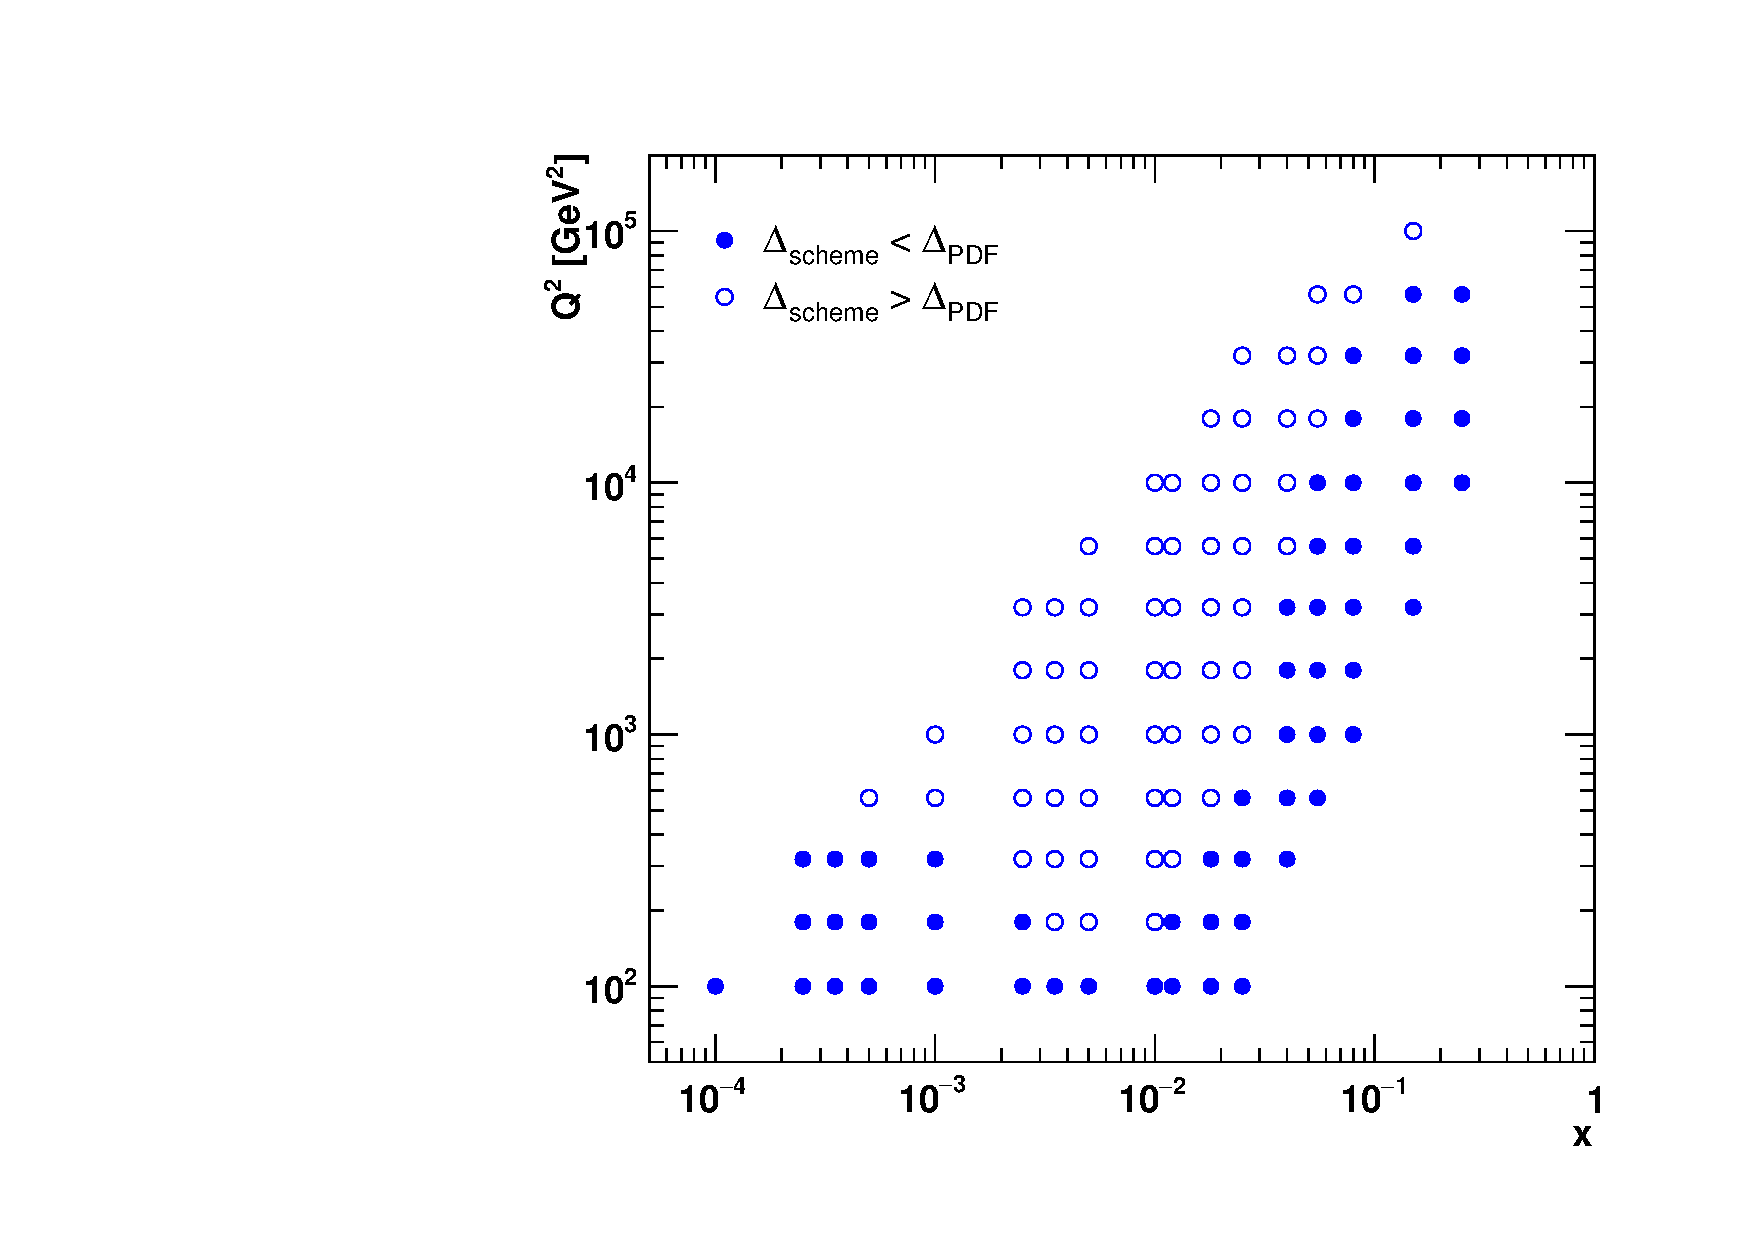
\includegraphics[width=0.5\textwidth]{pics/pseudodata.pdf}}}
  \caption{The full ($\Delta_{\rm scheme} < \Delta_{\rm PDF}$, $\Delta_{\rm scheme} > \Delta_{\rm PDF}$) and restricted ($\Delta_{\rm scheme} < \Delta_{\rm PDF}$) sets of data points which are used for PDF profiling.}
  \label{fig:data}
\end{figure}

\new{
Additionally, in the case of the NNPDF3.1 set, it is possible to check 
the constraints on the strange quark and anti-quark distributions 
separately, because no assumption $s=\bar{s}$ is used in NNPDF3.1. 
The LHeC $e^{-}p$ pseudodata provide direct constraints only on $\bar{s}$. 
Nevertheless due to the apparently strong correlation between $s$ and 
$\bar{s}$ in the NNPDF3.1 fit, quite strong constraints are present on both 
the $s$ and $\bar{s}$ distributions once the direct constraints on $\bar{s}$ 
are provided by the LHeC pseudodata. However, only mild constraints 
are put on the ratio $s/\overline{s}$. This indicates that for precise 
determination of $s/\overline{s}$ both $e^{-}p$ and $e^{+}p$ data will be needed.

\begin{figure}
  \centering
  {{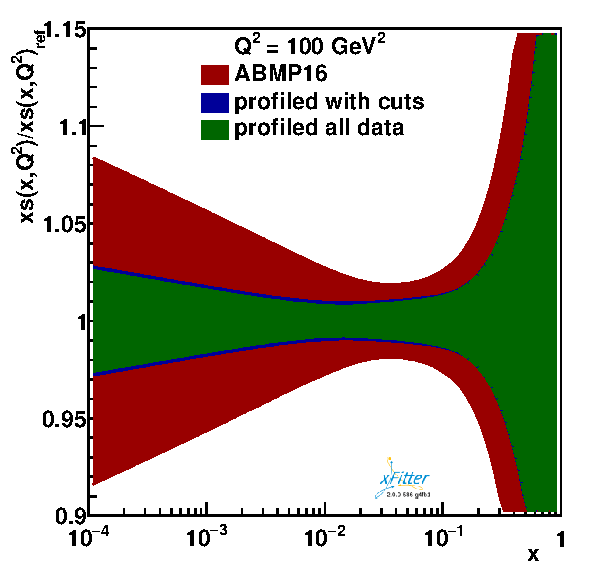
\includegraphics[width=0.235\textwidth]{pics/pdf-profile-ffabm/q2_100_pdf_sq_ratio.pdf}}}
  {{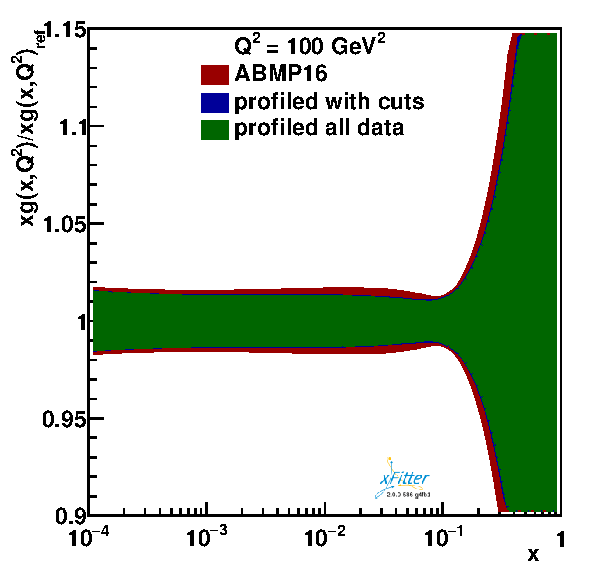
\includegraphics[width=0.235\textwidth]{pics/pdf-profile-ffabm/q2_100_pdf_g_ratio.pdf}}}\\
  {{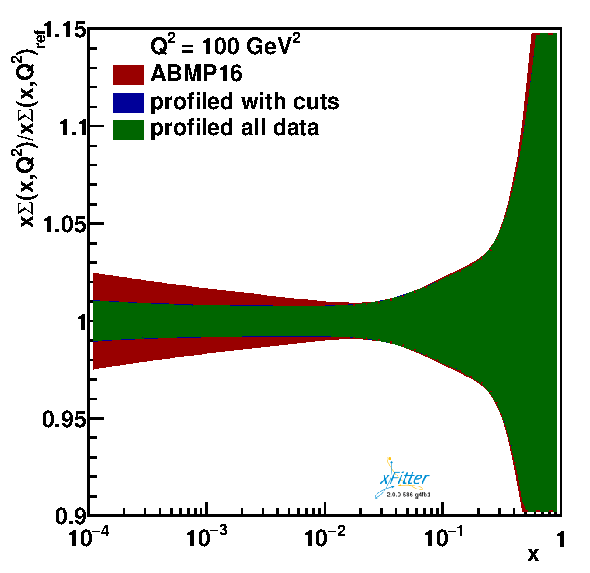
\includegraphics[width=0.235\textwidth]{pics/pdf-profile-ffabm/q2_100_pdf_Sea_ratio.pdf}}}
  {{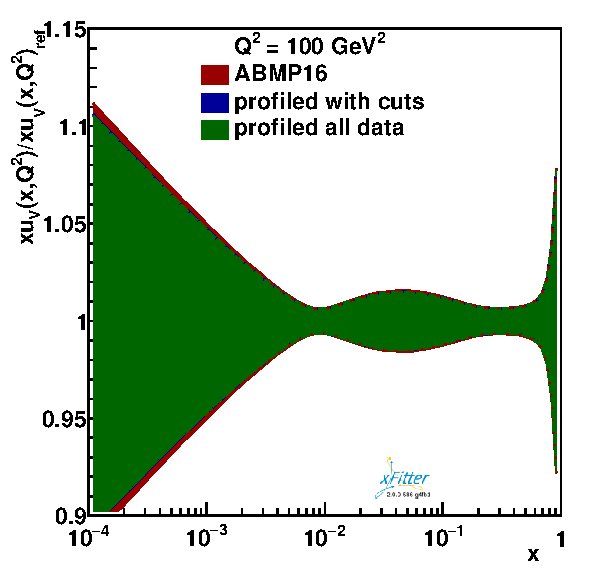
\includegraphics[width=0.235\textwidth]{pics/pdf-profile-ffabm/q2_100_pdf_uv_ratio.pdf}}}
  {{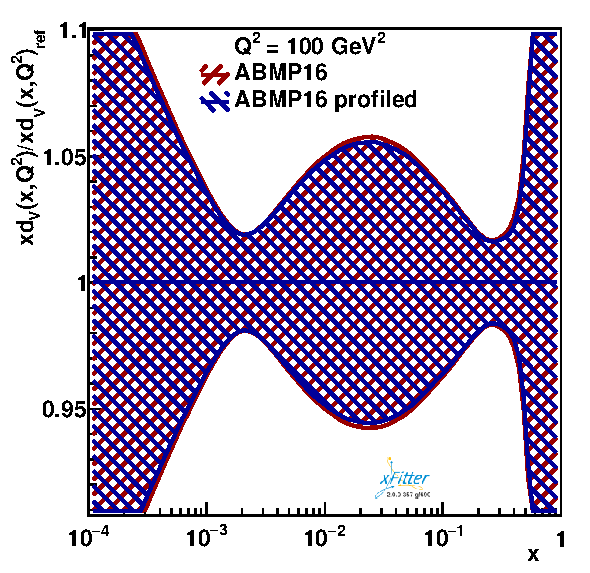
\includegraphics[width=0.235\textwidth]{pics/pdf-profile-ffabm/q2_100_pdf_dv_ratio.pdf}}}
  \caption{The relative strange (top left), gluon (top right), sea
    quark (middle left), u valence quark (middle right) and d valence
    quark (bottom) PDF uncertainties at $\mu_\mathrm{f}^2=100$ GeV$^2$
    of the original and profiled \abmp PDF set.}
  \label{fig:pdf-abmp}
\end{figure}

\begin{figure}
  \centering
  {{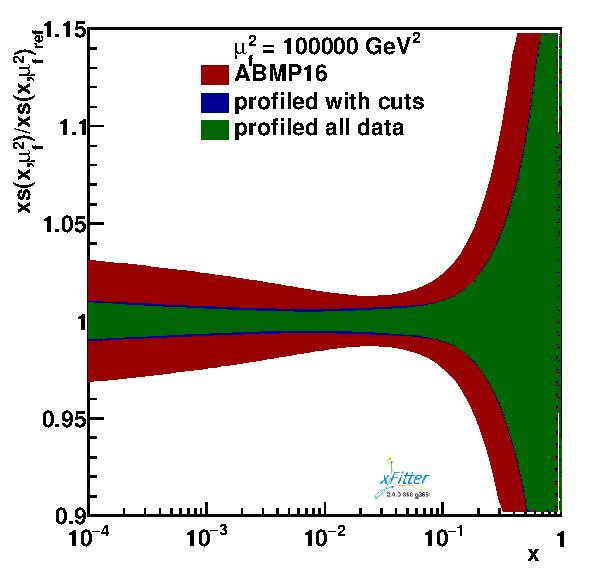
\includegraphics[width=0.235\textwidth]{pics/pdf-profile-ffabm/q2_100000_pdf_sq_ratio.pdf}}}
  {{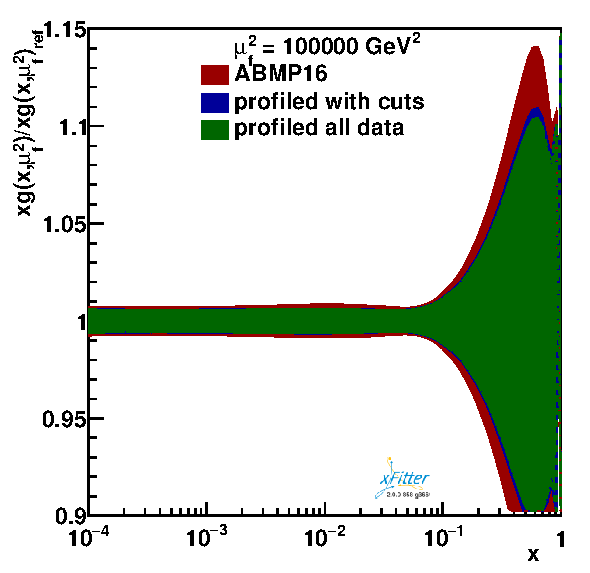
\includegraphics[width=0.235\textwidth]{pics/pdf-profile-ffabm/q2_100000_pdf_g_ratio.pdf}}}\\
  {{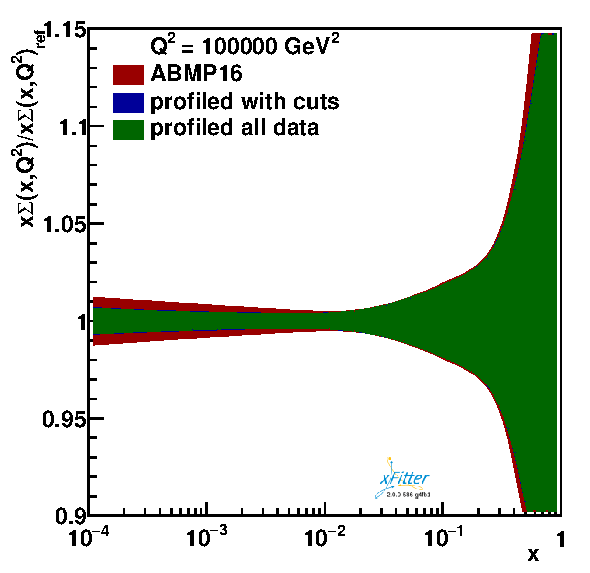
\includegraphics[width=0.235\textwidth]{pics/pdf-profile-ffabm/q2_100000_pdf_Sea_ratio.pdf}}}
  {{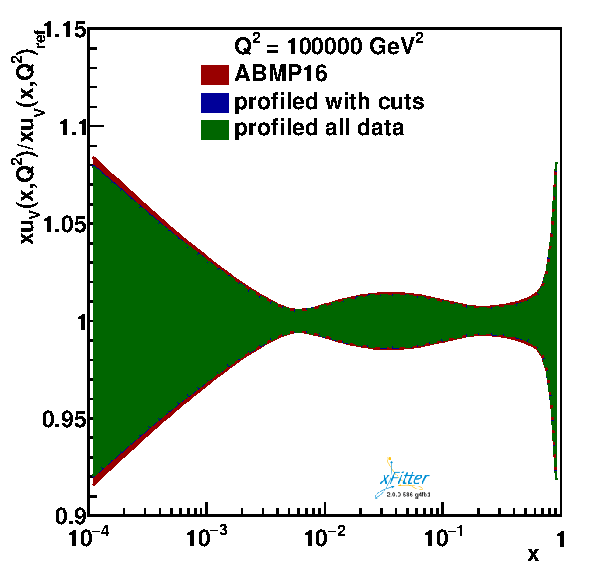
\includegraphics[width=0.235\textwidth]{pics/pdf-profile-ffabm/q2_100000_pdf_uv_ratio.pdf}}}
  {{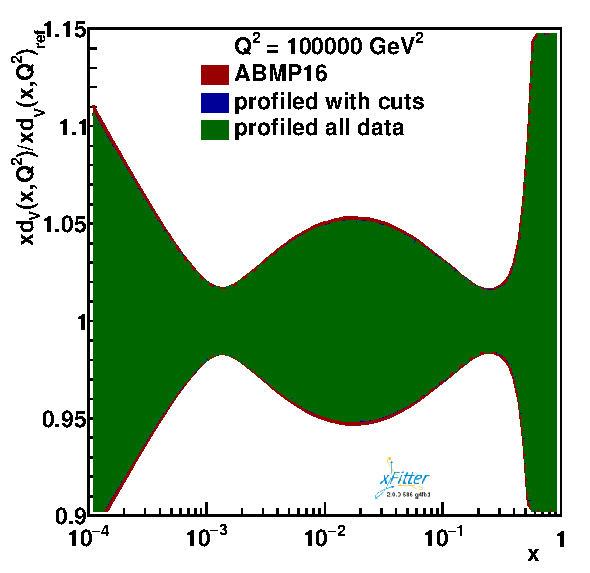
\includegraphics[width=0.235\textwidth]{pics/pdf-profile-ffabm/q2_100000_pdf_dv_ratio.pdf}}}
  \caption{The relative strange (top left), gluon (top right), sea
    quark (middle left), u valence quark (middle right) and d valence
    quark (bottom) PDF uncertainties at $\mu_\mathrm{f}^2=100000$
    GeV$^2$ of the original and profiled \abmp PDF set.}
  \label{fig:pdf-abmp-100000}
\end{figure}

\begin{figure}
  \centering
  {{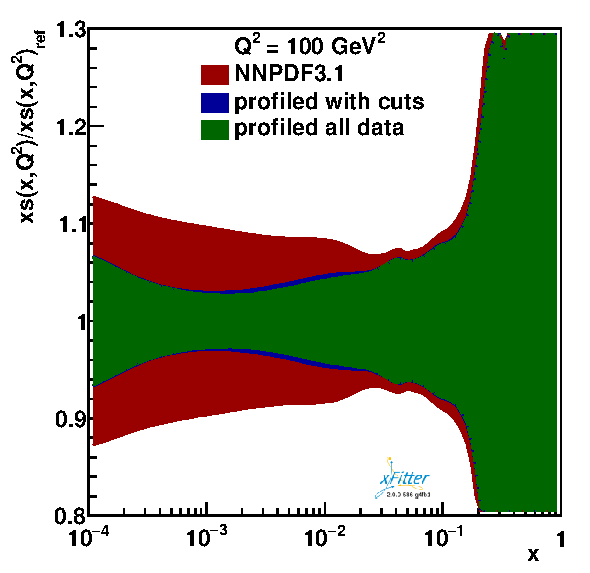
\includegraphics[width=0.235\textwidth]{pics/pdf-profile-fonll/q2_100_pdf_sq_ratio.pdf}}}
  \put(-95,95){(a)}
  {{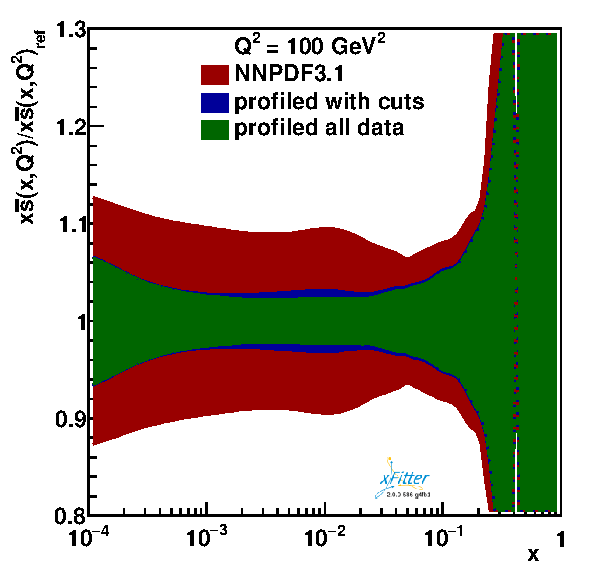
\includegraphics[width=0.235\textwidth]{pics/pdf-profile-fonll/q2_100_pdf_sbar_ratio.pdf}}}
  \put(-95,95){(b)}\\
  {{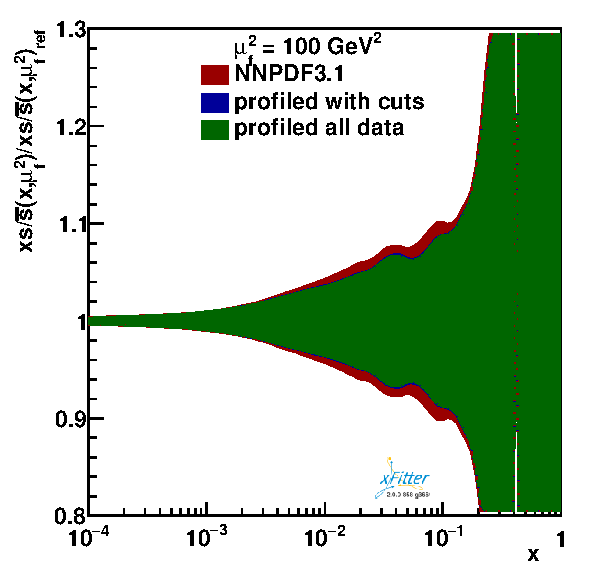
\includegraphics[width=0.235\textwidth]{pics/pdf-profile-fonll/q2_100_pdf_soversbar_ratio.pdf}}}
  \put(-95,95){(c)}
  {{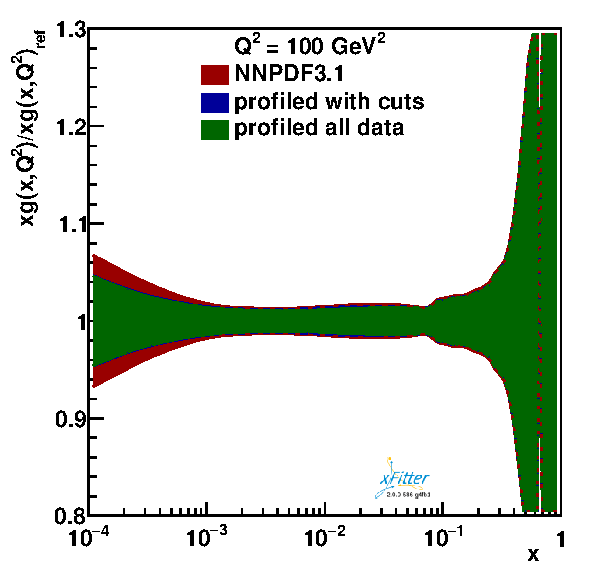
\includegraphics[width=0.235\textwidth]{pics/pdf-profile-fonll/q2_100_pdf_g_ratio.pdf}}}
  \put(-95,95){(d)}\\
  {{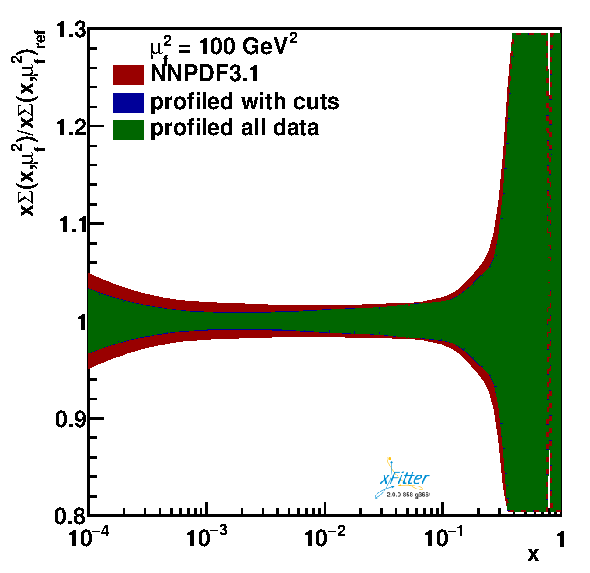
\includegraphics[width=0.235\textwidth]{pics/pdf-profile-fonll/q2_100_pdf_Sea_ratio.pdf}}}
  \put(-30,95){(e)}
  {{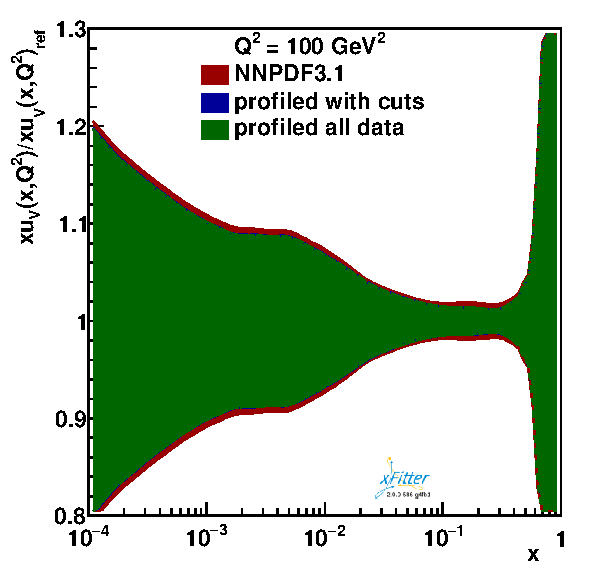
\includegraphics[width=0.235\textwidth]{pics/pdf-profile-fonll/q2_100_pdf_uv_ratio.pdf}}}
  \put(-95,95){(f)}\\
  {{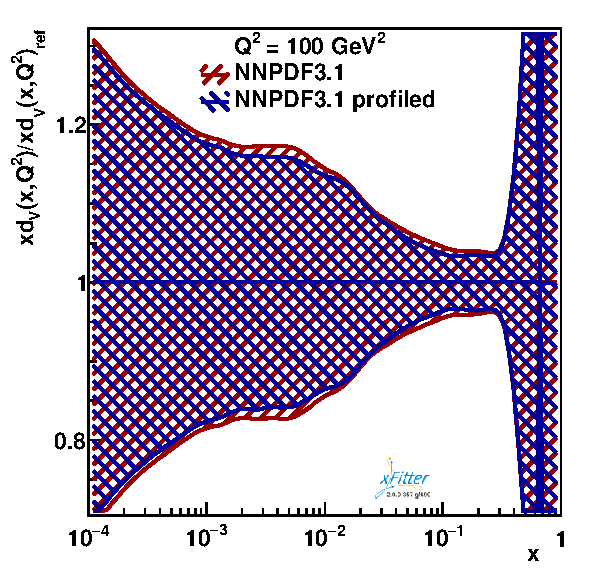
\includegraphics[width=0.235\textwidth]{pics/pdf-profile-fonll/q2_100_pdf_dv_ratio.pdf}}}
  \put(-30,95){(g)}
  {{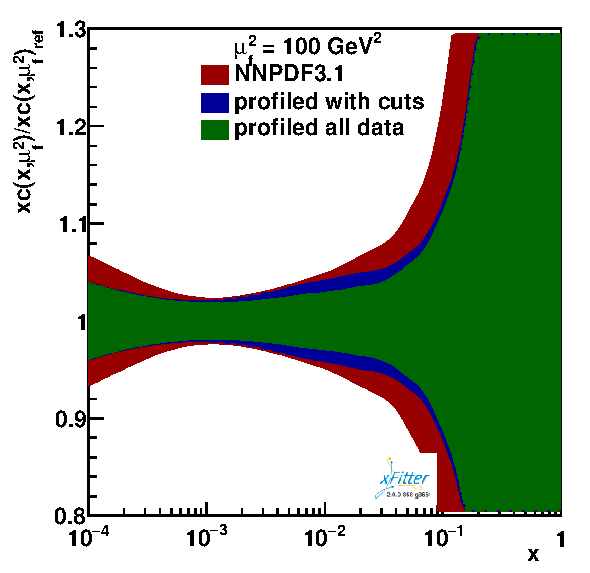
\includegraphics[width=0.235\textwidth]{pics/pdf-profile-fonll/q2_100_pdf_c_ratio.pdf}}}
  \put(-95,95){(h)}
  \caption{The relative strange quark (a), strange anti-quark (b), and ratio $s/\overline{s}$ (c), gluon (d), sea
    quark (e), u valence quark (f), d valence quark (g) and charm quark (h) PDF
    uncertainties at $\mu_\mathrm{f}^2=100$ GeV$^2$ of the original
    and profiled \nnpdf PDF set.}
  \label{fig:pdf-nnpdf}
\end{figure}

\begin{figure}
  \centering
  {{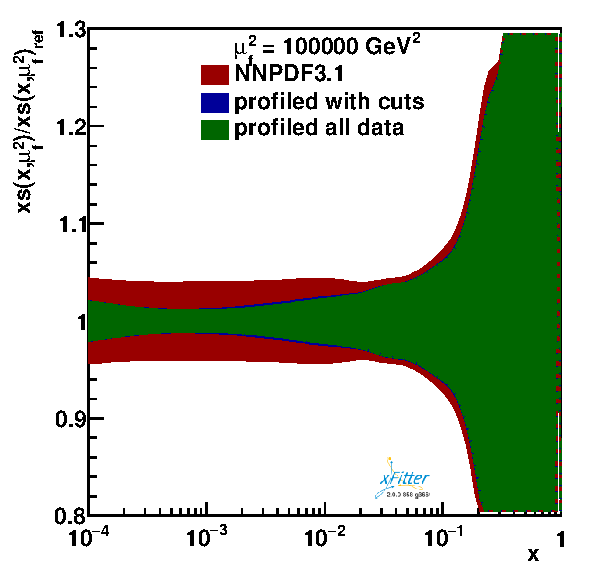
\includegraphics[width=0.235\textwidth]{pics/pdf-profile-fonll/q2_100000_pdf_sq_ratio.pdf}}}
  \put(-95,95){(a)}
  {{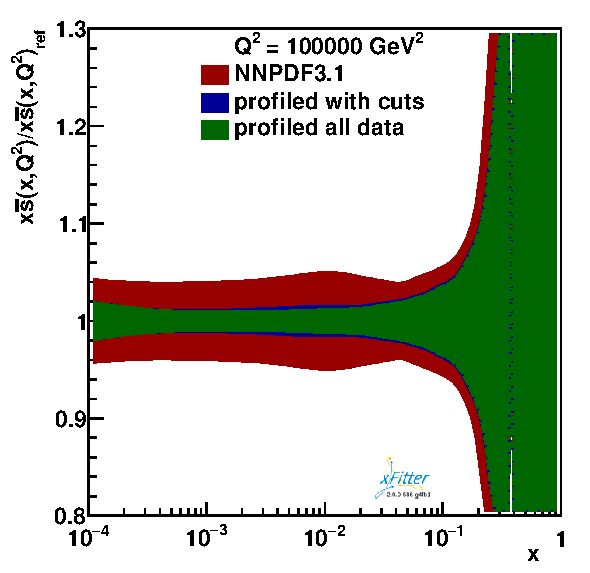
\includegraphics[width=0.235\textwidth]{pics/pdf-profile-fonll/q2_100000_pdf_sbar_ratio.pdf}}}
  \put(-95,95){(b)}\\
  {{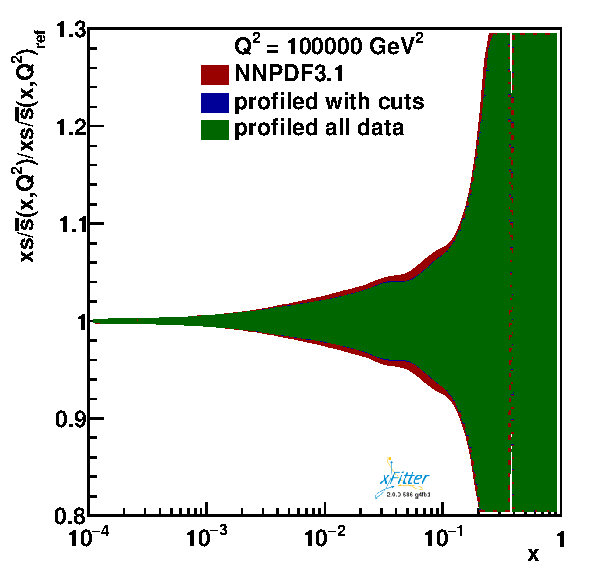
\includegraphics[width=0.235\textwidth]{pics/pdf-profile-fonll/q2_100000_pdf_soversbar_ratio.pdf}}}
  \put(-95,95){(c)}
  {{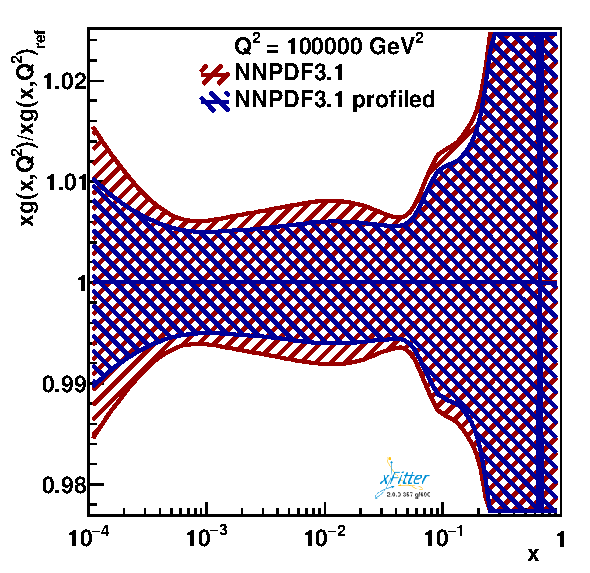
\includegraphics[width=0.235\textwidth]{pics/pdf-profile-fonll/q2_100000_pdf_g_ratio.pdf}}}
  \put(-95,95){(d)}\\
  {{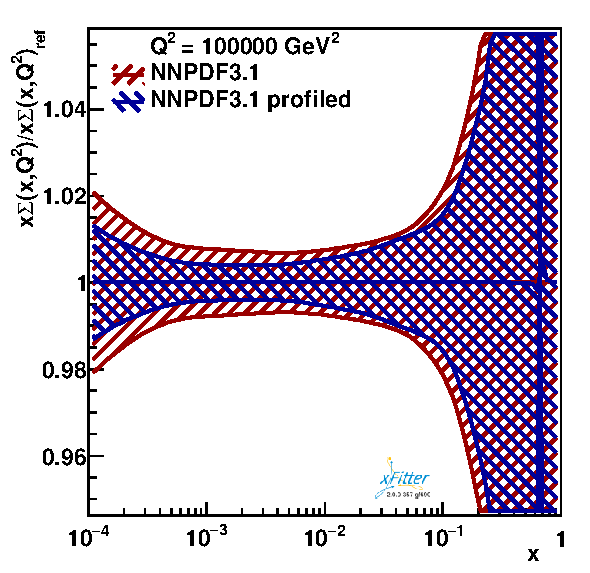
\includegraphics[width=0.235\textwidth]{pics/pdf-profile-fonll/q2_100000_pdf_Sea_ratio.pdf}}}
  \put(-30,95){(e)}
  {{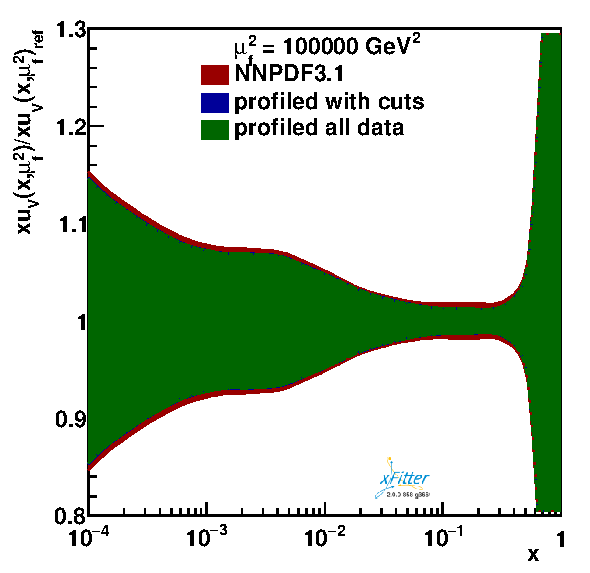
\includegraphics[width=0.235\textwidth]{pics/pdf-profile-fonll/q2_100000_pdf_uv_ratio.pdf}}}
  \put(-95,95){(f)}\\
  {{\includegraphics[width=0.235\textwidth]{pics/pdf-profile-fonll/q2_100000_pdf_dv_ratio.pdf}}}
  \put(-30,95){(g)}
  {{\includegraphics[width=0.235\textwidth]{pics/pdf-profile-fonll/q2_100000_pdf_c_ratio.pdf}}}
  \put(-95,95){(h)}
  \caption{The relative strange quark (a), strange anti-quark (b), and ratio $s/\overline{s}$ (c), gluon (d), sea
    quark (e), u valence quark (f), d valence quark (g) and charm quark (h) PDF
    uncertainties at $\mu_\mathrm{f}^2=100000$ GeV$^2$ of the original
    and profiled \nnpdf PDF set.}
  \label{fig:pdf-nnpdf-100000}
\end{figure}
}


%\textcolor{blue}{
  Comparing the results of profiled PDFs in the FFNS and the VFNS, we
find both analyses are able to significantly improve the constraints
on the strange quark PDF.  This result gives us confidence that the
general features we observe here are independent of the details of the
heavy flavor scheme.
%} %%%% end blue color


\goodbreak
\newpage
%%%%%%%%%%%%%%%%%%%%%%%%%%%%%%%%%%%%%%%%%%%%%%%%%%55
\section{Discussion and summary}
\label{sec:discuss}

%% MOTIVATION
%
The recent performance of the LHC has exceeded expectations and
produced an unprecedented number of precision measurements to be
analyzed; thus, it is essential to improve the theoretical
calculations to match.
%
The uncertainty for many of these precision measurements stems
primarily from the PDFs.
%
Hence, our ability to fully characterize the Higgs boson and constrain
beyond-standard-model (BSM) signatures ultimately comes down to how
accurately we determine the underlying PDFs; this has been the objective of this
study.

%% VALUE OF THE STRANGE QUARK
%
We have focused on the  strange-quark distribution which,
at the LHC, can have a significant impact on the $W/Z$ cross section:
one of the ``standard candle'' measurements.
%
If we can reduce the uncertainty for these predictions, we can set
stringent limits on any admixture of physics at higher scales.
%
Unfortunately, at present the strange PDF has a comparably large uncertainty
because measurements from the LHC and HERA, as well as older
fixed-target experiments, do not seem to provide a definitive result
for this flavor component.

This situation  has  prompted us to examine the CC DIS charm production at
the LHeC to determine the impact of this data set on the PDF
uncertainty.
%
We considered the LHeC  as this  high-energy $ep/A$
facility  could potentially run in parallel with the LHC and
provide insights into these issues at low $x$ and high $Q^2$ in advance of a FCC program.



% XFITTER CASE STUDY
%
This case study of the CC DIS charm production at the LHeC provides a
practical illustration of the many features of \xfitter.
%
As the \xfitter framework is designed to be a versatile open-source
software framework for the determination of PDFs and the analysis of
QCD physics, we can readily adapt this tool to address the impact and
influence of new data sets.
%
Furthermore, as both FFNS and VFNS calculations are implemented, we
can use \xfitter as a theoretical ``laboratory'' to study the
resummation of large logarithms and multi-scale issues.
%
We have outlined some of these issues in the Appendix.
%
In particular, the CC DIS charm production involves a flavor-changing
$W^\pm$ boson, multiple quark masses enter the calculation, and this
introduces some subtle theoretical issues to properly address the
disparate mass and energy scales.





%% LHeC RESULTS
%
Using the \xfitter framework, 
we find that the LHeC can provide strong constraints on the
strange-quark PDF, especially in the previously unexplored small-\xbj
region.\footnote{In this study we have focused exclusively on the LHeC
  result for CC DIS charm production; however, the LHeC has a broad
  multi-faceted program which is described in
  Refs.~\cite{AbelleiraFernandez:2012ty,Klein:2018rhq}.}
%
\new{A large reduction of uncertainties is observed also when restricting 
the input data to the kinematic range where the differences between the \ffns and 
\fonll schemes are not larger than the present PDF uncertainties, indicating 
that the obtained  PDF constraints are stable and 
independent of the particular heavy-flavor scheme.}
As noted above, a reduction of the strange-PDF uncertainties
influences the $W/Z$ production, and thus the Higgs production; hence,
the LHeC CC DIS charm production data represent a valuable addition
for the future global PDF fits.


\new{However, since charm CC production in $e^{-}p$ 
collisions mostly probe $\bar{s}$, only mild constraints are put on
the ratio $s/\overline{s}$ 
using the NNPDF3.1 PDF set as reference; therefore for a precise 
determination of this ratio, both $e^{-}p$ and $e^{+}p$ data will be needed.}





% CONCLUSION
%
In conclusion, we find that CC DIS charm production at the LHeC can
provide strong constraints on the strange PDF which are complementary
to the current data sets.
%
As the PDF uncertainty is the dominant factor for many precision
analyses, a reduction of these uncertainties will allow for more
accurate predictions which can be used to constrain both SM and BSM
physics processes.




%%%%%%%%%%%%%%%%%%%%%%%%%%%%%%%%%%%%%%%%%%%%%%%%%%%%%%%%%%%%5
\begin{acknowledgements}
\begin{hyphenrules}{nohyphenation}
    
We would like to thank
Max Klein for providing the pseudodata, and 
John~C.~Collins,
Aleksander~Kusina,
Ted~C.~Rogers,
Ingo~Schienbein,
George~Sterman,
for useful discussion.
The work of O.\,Z. has been supported by Bundesministerium f\"ur Bildung und Forschung (contract 05H18GUCC1).
This work F.\,O. was supported by the U.S. Department of Energy under Grant No. DE-SC0010129.

%  We would like to thank Juan Rojo for a cri\-ti\-cal reading of this
%  paper, and Luca Rottoli for discussions on the description of charm
%  data.  V.~B.\ and F.~G.\ are supported by the European Research
%  Council Starting Grant ``PDF4BSM''.  Additional support was received
%  by A.~G., A.~S.\ and P.~S.\ from the BMBF-JINR cooperation program
%  and the Heisenberg-Landau program.  A.~L.\ is supported by the
%  Polish Ministry under program Mobility Plus, no 1320/MOB/IV/2015/0.
%  M.~B.\ is supported by the by the Marie Sk\l{}odowska Curie grant
%  HiPPiE@LHC.

\end{hyphenrules}
\end{acknowledgements}

%%%%%%%%%%%%%%%%%%%%%%%%%%%%%%%%%%%%%%%%%
%  %% LyX 2.3.1 created this file.  For more info, see http://www.lyx.org/.
%  %% Do not edit unless you really know what you are doing.
%  \documentclass[twocolumn,english,showpacs,preprintnumbers,amsmath,amssymb,floatfix]{revtex4-1}
%  \usepackage[T1]{fontenc}
%  \usepackage[latin9]{inputenc}
%  \setcounter{secnumdepth}{3}
%  \usepackage{color}
%  \usepackage{babel}
%  \usepackage{graphicx}
%  \usepackage{esint}
%  \usepackage[unicode=true,
%   bookmarks=false,
%   breaklinks=false,pdfborder={0 0 1},backref=section,colorlinks=false]
%   {hyperref}
%  
%  \makeatletter
%  %%%%%%%%%%%%%%%%%%%%%%%%%%%%%% User specified LaTeX commands.
%  \hyphenpenalty=10000
%  
%  \makeatother
%  
%  \begin{document}
%  
\clearpage
\newcommand{\xsec}[1]{\vskip 6pt \noindent {\bf #1} \quad }

\appendix

{\small
\textbf{\textcolor{blue}{TO DO LIST:}}
\textcolor{blue}{{*} Follow up on John Collins' list {[}MOSTLY DONE{]} }
\textcolor{blue}{{*} Add brief mention at end that this applies also
to bottom quark {[}at end{]}}
\textcolor{blue}{{*} refs from Sasha: LHC W+c measurements:
  \cite{Chatrchyan:2013uja,Aad:2014xca,Sirunyan:2018hde}}
  }

\section{$F_{2}^{charm}$ Beyond Leading-Order}

\begin{figure}
\centering \includegraphics[clip,width=0.45\textwidth]{pics/fred/acot_fig}
\caption{Calculation of $F_{2}^{c}$ vs.\ $\mu$ in the VFNS illustrating the
cancellation of the LO ($\bar{c}W^{+}\to\bar{s}$) and the SUB \hbox{$(g\to \bar{c})$}$\otimes$\hbox{$(\bar{c}W^+ \to \bar{s})$}
contributions in the region $\mu\sim m_{c}$. The $Q$ scale is fixed
at $10\,$GeV and the charm PDF is matched at $\mu_{c}=m_{c}$ such
that $f_{c}(x,\mu=m_{c})=0$. \label{fig:acot}}
\end{figure}

\begin{figure*}
\centering \includegraphics[clip,width=0.8\textwidth]{pics/fred/tchannel}
\caption{Gluon $t$-channel processes up to ${\cal  O}(\alpha_S^1)$.  \label{fig:tchannel}}
\end{figure*}

\begin{figure*}
\centering \includegraphics[clip,width=0.8\textwidth]{pics/fred/uchannel}
\caption{Gluon NLO $u$-channel processes  up to ${\cal  O}(\alpha_S^1)$. \label{fig:uchannel}}
\end{figure*}




\xsec{The Multi-Scale Problem:}
%
The charged current DIS charm production process involves some interesting
issues that we will explore here in detail. In particular, there are
multiple mass and energy scales which span a wide kinematic range,
and it becomes an intricate puzzle to treat them all properly. 

For this current illustration, we will focus on the contribution to
the DIS $F_{2}^{c}$ structure function from the process involving
the strange and charm quark; other quark combinations can be addressed
in a similar manner. In particular, we will show that as we go to
higher-orders the $F_{2}^{c}$ structure function must be defined
carefully so that i) theoretically it is free of divergences and independent
of the renormalization scales, and ii) experimentally it matches what
is measured by the detector.

\xsec{Overview:}
%

\textcolor{blue}{... to be filled in ... (what other detailed are needed???)}

\xsec{The Mass Scales:}
%
There are four mass scales that enter this process: $\{Q,\mu,m_{s},m_{c}\}$;
additionally, in the case of the VFNS we have the matching scale,
$\mu_{c}$.

The $Q$ scale is the invariant mass of the virtual boson probe ($W^{+}$
in this case), and can be related to the energy and angle of lepton;
this is a physically measurable kinematic variable. 

In contrast, the renormalization scale $\mu$ is an unphysical scale
used to factorize the PDF and the hard scattering cross section; thus,
the physics should be insensitive to a variation of $\mu$. As our
calculations typically involve the dimensionless combination $\ln(\mu^{2}/Q^{2})$,
we generally choose $\mu\sim Q$ avoid large logarithms. 

The strange quark is a ``light'' active parton with an associated
PDF $s(x)$ and mass $m_{s}$. The strange quark mass is comparable
or less than other hadronic scales which are neglected; as such, it
serves only as a regulator and plays no physical role, and we can
take $m_{s}\to0$ if we choose. 

The charm quark is a ``heavy'' object; its associated mass $m_{c}$
does play a physical role and cannot be neglected. There may or may
not be a PDF associated with the charm. In a 3-flavor FFNS scheme,
there is no charm PDF. In a 4-flavor VFNS there is a charm PDF only
when the $\mu$ scale is above the scale where the charm PDF is activated;
we call this the matching scale, $\mu_{c}$. It is common\footnote{The choice of matching scale $\mu_{c}=m_{c}$ is common because at
NLO the $\overline{MS}$ matching conditions on the PDFs are proportional
to the DGLAP kernel times $\ln(\mu/m_{c})$, as explicit calculation
shows the constant term vanishes; thus we have the simple boundary
condition $f_{c}(x,\mu=m_{c})=0$. At NNLO, the constant term is non-zero
and this yields $f_{c}(x,\mu=m_{c})\not=0$. See \cite{Stavreva:2012bs}
and references therein.} to set $\mu_{c}=m_{c}$, but this is not required.\footnote{By displacing the matching scale to larger values $\mu_{c}\gg m_{c}$,
can have the advantage of avoiding delicate cancellations in the region
$\mu\sim m_{c}$; this flexibility was explored in Refs.~\cite{Bertone:2017ehk,Bertone:2018ids}
.} In this study we will fix the matching scale to this common choice:
$\mu_{c}=m_{c}$.



What makes this process complex is there is no fixed hierarchy for
the mass scales, and we will need to compute both in the low $Q$
region where $Q\lesssim m_{c}$ as well as the high $Q$ region $Q\gg m_{c}$. 



Because there are two different quark masses $\{m_{s},m_{c}\}$ involved
in the charged current DIS flavor-changing process,  we can examine
the mass singularities of the $t$-channel and $u$-channel separately.
This separation is particularly useful to understand how the individual
mass singularities are addressed, and how FFNS and VFNS organize the
contributions to the total structure function. 

\xsec{3-Flavor FFNS:}
%
To be specific, we will consider charged-current DIS production of
a charm quark. We first compute this in a 3-flavor (FFNS) scheme where
$\{u,d,s\}$ are light ``active'' partons in the proton, and charm
$\{c\}$ is considered an external ``heavy'' particle. This can
be implemented in the ACOT scheme\cite{Aivazis:1993pi} for example
by using a CWZ renormalization\cite{Collins:1978wz} where the light
``active'' partons are renormalized with normal $\overline{MS}$,
and the ``heavy'' quarks use a zero-momentum subtraction. In this
scheme, the \textbf{leading-order} (LO) process is \mbox{$sW^{+}\to c$}
as illustrated in Fig.\,\ref{fig:acot}. At \textbf{next-to-leading-order}
(NLO), we then include \mbox{$gW^{+}\to c\bar{s}$} which has both $t$-channel
and $u$-channel contributions.\footnote{Note, there are also corresponding quark-initiated processes; we will
focus on the gluon-initiated processes as this is sufficient to illustrate
our points. Both the gluon- and quark-initiated contributions are
included in our calculations. }

\xsec{$t$-Channel:}
%
The $t$-channel process has an intermediate $s$-quark exchanged, and
if we use the strange quark mass $m_{s}$ to regulate the singularities,
this will yield a contribution proportional to $\ln(Q/m_{s})$. This
mass singularity arises from the region of phase space where the exchanged
$s$-quark becomes collinear and close to the mass-shell; that is,
when the phase space of the \mbox{$gW^{+}\to c\bar{s}$} process begins to
overlap with that of the \mbox{$sW^{+}\to c$} process. This ``double counting''
is resolved by a \textbf{subtraction} (SUB) counter-term
%(which is formally part of the NLO contribution)
given by:
\[
(SUB)\sim f_{g}\otimes\widetilde{f}{}_{g\to s}\otimes\sigma_{sW^{+}\to c}\quad.
\]
Here, $\widetilde{f}{}_{g\to s}$ is the perturbative splitting of
the gluon into an $s\bar{s}$ pair; the leading term is proportional
to:\footnote{The scale of the SUB term is $\mu$ as the relevant scale here is
the renormalization scale of the PDF:$f(x,\mu)\otimes\hat{\sigma}(x,Q,\mu)$. }
\[
\widetilde{f}_{g\to s}(x,\mu)\sim\frac{\alpha_{S}(\mu)}{2\pi}P_{g\to s}^{(1)}(x)\:\ln\left(\frac{\mu^{2}}{m_{s}^{2}}\right)+\text{{\cal O}}(\alpha_{s}^{2})
\]
 where $P_{g\to s}^{(1)}(x)$ is the $\alpha_{S}^{1}$ DGLAP splitting
kernel for \hbox{$g\to s$}.

The complete contribution to the structure function is given by:
\[
F_{2}^{c}\sim TOT=LO+(NLO-SUB)
\]
The complete ${\cal O}(\alpha_{s}^{1})$ contribution is the combination
$(NLO-SUB)$; our separation into $NLO$ and $SUB$ is simply to illustrate
the interplay of these components. Both the NLO and SUB terms have
$\ln(m_{s})$ divergences, but these precisely cancel and yield a
well defined result even as we take the $m_{s}\to0$ limit.\footnote{In fact, we could have taken $m_{s}=0$ initially and used dimensional
regularization to compute the contributions.}

\xsec{$u$-Channel:}
%
We next examine the $u$-channel NLO contribution to the \mbox{$gW^{+}\to c\bar{s}$}
process. This has an intermediate $c$-quark exchanged, and is proportional
to $\ln(Q/m_{c})$. In the FFNS where the charm is a ``heavy'' non-parton,
there is no counter-term for this graph, and the resulting observables
will retain the $\ln(Q/m_{c})$ dependence. In principle, this means
when we go to large $Q$-scales, these terms will begin to degrade
the convergence of our perturbation series. In practice, while this
degradation only grows logarithmically, at large scales (such as at
the LHC) we do find it convenient to treat the charm on an equal-footing
as the ${u,d,s}$ partons. 

\xsec{4-Flavor VFNS:}
%
We now turn to the 4-flavor (VFNS) scheme where we include the charm
quark as an ``active'' parton and compute its associated PDF.

In this case, there is a $u$-channel counter-term (SUB) given by $f_{g}\otimes\widetilde{f}{}_{g\to\bar{c}}\otimes\sigma_{\bar{c}W^{+}\to\bar{s}}$
which is proportional to $\ln(\mu/m_{c})$. The NLO $u$-channel contribution
will have a $\ln(Q/m_{c})$ contribution, so the combination $(NLO-SUB)$
is also free of mass singularities.\footnote{Specifically, the combination $(NLO-SUB)$ is free of mass singularities
and finite in the limit $m_{c}\to0$. Note, the VFNS fully retains
the charm quark mass $m_{c}$ and (in contrast to some claims in the
literature) the factorization holds up to ${\cal O}(\Lambda^{2}/Q^{2})$
corrections; all terms of order $(m_{c}^{2}/Q^{2})$ are fully included.\cite{Collins:1998rz}}

What is less obvious is that we also must include the LO process \mbox{$\bar{c}W^{+}\to\bar{s}$}.
There are two ways we can understand why this is necessary. 

\xsec{Explanation \#1: Matching of LO and SUB:}
%
Recall that in the $t$-channel case, the subtraction term SUB removed
the double counting between the LO \mbox{$sW^{+}\to c$} and NLO \mbox{$gW^{+}\to c\bar{s}$}
processes. 

The $u$-channel case is analogous in that this subtraction term removes
the double counting between the LO \mbox{$\bar{c}W^{+}\to\bar{s}$} and NLO
\mbox{$gW^{+}\to c\bar{s}$} processes; both contributions are required to
ensure the resulting cross section is insensitive to the $\mu$-scale. 

This is apparent in Fig.~\ref{fig:acot} where we plot the individual
terms versus the $\mu$ scale for a fixed $x$ and $Q$. In the region
of $\mu\sim m_{c}$, the charm PDF $f_{c}(x,\mu)$ (and hence, the
LO contribution) rises very quickly as the DGLAP evolution is driven
by the very large gluon via $g\to c\bar{c}$ splitting, and combined
with a large $\alpha_{S}(\mu)$. The SUB subtraction also rises quickly
as this is driven by the logarithmic term $\ln(\mu^{2}/m_{c}^{2})$.
The difference \mbox{$(LO-SUB)$} is the physical contribution to the total
\mbox{$[TOT=LO+NLO-SUB]$}, and it is this combination which is smooth across
the ``turn on'' of the charm PDF at the matching scale $\mu_{c}=m_{c}$.
We now see that if we neglect the LO \mbox{($\bar{c}W^{+}\to\bar{s}$)} contribution,
we lose the cancellation between LO and SUB in the region $\mu\sim m_{c}$,
and our structure function (or cross section) would have an anomalous
shift at the arbitrarily location $(\mu_{c})$ where we turn on the
charm PDF. 

As we vary the unphysical renormalization scale $\mu$, we are simply
shifting contributions between the separate \mbox{$\{LO,NLO,SUB\}$} terms
which individually exhibit a large $\mu$-dependence. However, the
total combination $(TOT)$ which represents the physical observable
is relatively insensitive to $\mu$ (up to higher orders), and this
property is evident in Fig.~\ref{fig:acot}.

\xsec{Explanation \#2: Removing ``Double Counting:''}
%
A second way to understand why we require the LO process \mbox{$\bar{c}W^{+}\to\bar{s}$}
is to consider the regions of phase space covered by each of the sub-processes.
The singularity of the $u$-channel NLO \mbox{$gW^{+}\to c\bar{s}$} processes
arises the phase space region when the intermediate $\bar{c}$ quark
becomes collinear and close to the mass-shell.\footnote{Specifically, the charm quark is off-shell by the order of its mass
$m_{c}$; this is independent of the scale $Q$ and \textbf{\textit{does
not}} assume any $Q\gg m_{c}$ limit. } This is precisely the phase space region of the LO process \mbox{$\bar{c}W^{+}\to\bar{s}$}
where the partonic $\bar{c}$-quark is collinear to the hadron. The
SUB term then removes the ``double counting'' between the LO and
NLO contributions; hence, all three contributions \mbox{$\{LO,NLO,SUB\}$}
are necessary to cover the full phase space.

This is also apparent if we consider the transverse momentum $(p_{T})$
of the final-state charm in the Breit frame. For the LO \mbox{$\bar{c}W^{+}\to\bar{s}$}
process in the Breit frame, the incoming $W^{+}$ and $\bar{c}$ are
collinear, and the produced $\bar{s}$ must have zero $p_{T}$ in
this frame.

For the NLO $gW^{+}\to c\bar{s}$ process, we integrate over the complete
phase space for the exchanged $\bar{c}$ quark, and this will include
the region where the $\bar{c}$ quark is emitted nearly collinear
to the gluon and nearly on-shell; in this region the $\bar{c}$ quark
will have $p_{T}\sim0$ and we encounter a singularity from the internal
$\bar{c}$ propagator. The $p_{T}\sim0$ region is precisely that
subtracted by the SUB counter term,\footnote{Specifically, the incoming $W^{+}$ and $g$ are collinear, and the
gluon then emits a collinear $c\bar{c}$ pair so the final $\bar{s}$
has zero $p_{T}$.} and this ensure that the combination $(NLO-SUB)$ is free of divergences.



\xsec{Recap:}
%
To recap, i) the combination of the LO and SUB terms ensure a minimal
$\mu$-variation at low $\mu$ scales, and ii) the combination of
SUB and NLO ensure the mass singularities are canceled at high $\mu$
scales.

This interplay of the terms illustrates some of the intricacies of
QCD, especially since this exchange is across different orders of
$\alpha_{s}$.


Furthermore, note that in the $u$-channel for both the LO and SUB contributions,
the charm quark is collinear with the incoming hadron, and thus exits
in the hadron remnants. While this may be experimentally unobservable,
because we are asking for a \textit{``fully inclusive''} $F_{2}^{c}$,
these contributions cannot be simply ignored. We will discuss this
further in the following section. 

\xsec{Defining $F_{2}^{c}$:}
%
The $u$-channel LO \mbox{$\bar{c}W^{+}\to\bar{s}$} process foreshadows difficulties
we encounter if we try and extend the concept of a ``fully inclusive''
$F_{2}^{c}$ to higher orders. We note that in Ref.~\cite{Collins:1998rz}
Collins extended the proof of factorization to include heavy quarks
such as charm and bottom for an inclusive structure function $F_{2}$;
there is no corresponding proof for an \textit{``fully inclusive''}
$F_{2}^{c}$ because a well defined $F_{2}^{c}$ that is free of singularities
will depend on experimental cuts or theoretical regulators. The simplistic
definition that $F_{2}^{c}$ is the contribution to $F_{2}$ from
states with charm in the final state is not appropriate. 



The $F_{2}^{c}$ that is measured experimentally is a differential
cross section for producing a charm quark in the final state in a
fiducial region; as we go to higher orders, we must be careful how
we define this quantity so that it is singularity-free and $\mu$-independent. 



To characterize the problems in constructing a \textit{``fully inclusive''}
$F_{2}^{c}$, we can imagine starting from the (well defined) inclusive
$F_{2}$, and then dividing the contributions into two sets: one for
$F_{2}^{c}$ for the ``heavy'' charm quark, and the rest into $F_{2}^{u,d,s}$
for the ``light'' quarks. We will show this division cannot be performed
unambiguously.



The $u$-channel LO $\bar{c}W^{+}\to\bar{s}$ process does not have any
``apparent'' charm quark in the final state, but this contribution
is essential to balance with the SUB process
\mbox{$f_{g}\otimes\widetilde{f}{}_{g\to\bar{c}}\otimes\sigma_{\bar{c}W^{+}\to\bar{s}}$.}
Note that for the SUB process, the charm quark arises from a gluon
splitting into a collinear $c\bar{c}$ pair which is then part of
the hadron remnants. For the LO process, presumably our $\bar{c}$
quark also came from a gluon splitting into a collinear $c\bar{c}$
pair. Thus, if we want to define a\textit{ ``fully inclusive''}
$F_{2}^{c}$, it seems we must include those cases where the charm
in contained in the hadron remnants.

This issues touches on the fact that because the charm parton is not
observable, ultimately we must produce a charm meson (typically a
$D^{*}$) via a fragmentation process. This requires the introduction
of a set of fragmentation functions (FFs) which are scale-dependent
and will factorize final-state singularities in a similar manner as
the PDFs factor the initial-state singularities.\footnote{Also note, for the NLO quark-initiated contributions (not shown) we
will have final state singularities from processes such as $c\to cg$
which will be factorized into the fragmentation functions.} The attempt to define a \textit{``fully inclusive''} $F_{2}^{c}$
is further complicated by the fact that the FFs can produce a D{*}
from the fragmentation of a gluon or a light hadron.




\xsec{The Bubble  Diagram:}
%
\begin{figure}[t]
\centering \includegraphics[width=0.45\textwidth]{pics/fred/feyngraph}
\caption{A higher order Feynman graph illustrating the difficulty in defining
  a ``fully inclusive'' $F_{2}^{charm}$.
 A light quark ($q$)
 scatters from a vector boson ($V$) with 
 a $c\bar{c}$ in the internal loop.
 If we cut the amplitude at  ``A''
we have charm in the final state and this must be included in $F_{2}^{charm}$.
If we cut the amplitude with cut ``B'' there is no charm in the
final state, but this process is required to cancel the divergences.
Additionally, since this diagram contributes to the beta function,
this highlights the complications of using an $\alpha_{S}$ and hard
scattering $\hat{\sigma}$ with differing $N_{\rm eff}$. \label{fig:bubble}}
\end{figure}

Such difficulties of defining a \textit{``fully inclusive''} $F_{2}^{c}$
are not unique to the VFNS, and also are encountered in the FFNS.
This is succinctly illustrated in Fig.~\ref{fig:bubble} which shows
a higher-order DIS process with a quark--anti-quark loop. Let us
compute this diagram in a 3-flavor FFNS where the internal loop is
a $c\bar{c}$-pair, and the external quark is a light \mbox{$\{u,d,s\}$}.
If the final-state is represented by Cut-A, then we have charm quarks
in the final state, and this should be included in $F_{2}^{c}$. 

However, if we instead use Cut-B as the final state, there is no charm
in the final state, so this should not be included in $F_{2}^{c}$.
{[}More precisely, when we renormalize the charm loop with zero-momentum
subtraction, this contribution effectively decouples.{]} Thus, the
contribution from Cut-A will be included in $F_{2}^{c}$, but the
contribution from Cut-B will not. 


If we had included the contributions for both Cut-A and Cut-B, the
total would be free of divergences. The QED analog of this is the
well known Block-Nordsieck theorem,\cite{Bloch:1937pw} and the QCD
extensions were performed by Libby and Sterman.\cite{Libby:1978bx,Libby:1978nr}
For example, the bubble diagram of Fig.~\ref{fig:bubble} is encountered
in the $F_{2}^{c}$ heavy quark calculations of Refs.~\cite{Chuvakin:1999nx,Chuvakin:2000jm};
here, an additional scale $\Delta$ must be introduced to cut on the
invariant mass of the internal quark--anti-quark pair and regulate
the singularities. 



\xsec{The running $\alpha_{S}$ in the FFNS:}
%
The bubble diagram of Fig.~\ref{fig:bubble} also highlights the
difficulty of using a $N_{\rm eff}=3$ FFNS with an $N_{\rm eff}=4$ flavor
running $\alpha_{S}(\mu)$. In a $N_{\rm eff}=3$ FFNS, internal $c\bar{c}$
loops decouple from the theory and are not included in the calculation;
however, the $N_{\rm eff}=4$ $\beta$-function requires precisely these
$c\bar{c}$ loop contributions.\footnote{Note; this deficiency can in principle be patched order-by-order by
expanding the $\beta$-function and inserting the required terms at
each order~\cite{Napoletano:2014thesis,Bierenbaum:2009zt,Cascioli:2013era}. } Once again, we cannot unambiguously divide the inclusive $F_{2}$
into separate ``light'' and ``heavy'' quantities. 



\xsec{Extensions to bottom and top:}
%
While we have used the charm quark to illustrate these features, the
same properties can, in principle, be applied to both the bottom and
top quark.\footnote{Additionally, Collins specifically addressed the case of multiple
heavy quarks which can allow for both charm and bottom in a unified
framework; in contrast to some incorrect claims in the literature,
there is no difficulty including multiple heavy quarks. (C.f, Ref.~\cite{Collins:1998rz},
Sec.~IX.)} For the case of the bottom quark, the larger mass $m_{b}$ yields
a smaller $\alpha_{s}(\mu)$ for $\mu\sim m_{b}$ and the evolution
of $f_{b}(x,\mu)$ is thus reduced; nevertheless, for large scale
processes (such as the LHC) we often find it convenient to make use
of $f_{b}(x,\mu)$ and treat the 5-flavors on an equal footing. 
%
For the case of the top quark, the very large
mass $m_{t}$ yields a much smaller $\alpha_{s}(\mu)$  for $\mu\sim m_{t}$  and the evolution
of $f_{t}(x,\mu)$ is comparatively reduced.




\subsection*{Summary }

To properly define an $F_{2}^{c}$ at all orders, we must be careful
to match the theoretical quantity to what is actually measured experimentally.
This is more complex than simply asking for the portion of $F_{2}$
which has charm in the final state, and is an issue for both the FFNS
and VFNS. The experimental $F_{2}^{c}$ is a differential cross section
for producing a charm meson in a fiducial region; this physical observable
is singularity-free and $\mu$-independent. 

We can compute in the FFNS, but in the large energy limit, we encounter
$\ln(Q^{2}/m_{c}^{2})$ divergences and this, in part, contributes
to the observed differences at large $Q$ scales. 

The VFNS includes the charm quark as an active parton for $\mu$ scales
above a matching scale $\mu_{c}$. For large $Q$ scales, the mass
singularities of NLO and SUB will cancel to yield a result free of
divergences. For scales $\mu\sim m_{c}$, cancellation between the
LO and SUB contributions ensures minimal $\mu$ dependence; however,
as this can be delicate to implement numerically, we have the option
of displacing the matching scale $\mu_{c}$ to a larger scale where
the cancellation is more stable.\cite{Bertone:2017ehk,Bertone:2018ids}


%\subsection*{Acknowledgements}
%Thanks to:
%John Collins, Ted Rogers, George Sterman, Ingo Schienbein, Aleksander Kusina

%\bibliographystyle{unsrt}
%\bibliography{fred}

%\end{document}

%%%%%%%%%%%%%%%%%%%%%%%%%%%%%%%%%%%%%%%%%

\bibliographystyle{spphys}
\bibliography{c_cpaper,extra}

\end{document}

